\documentclass{article}
\usepackage[utf8]{inputenc}
\usepackage[a4paper, total={6in, 9in}]{geometry}
\usepackage{amsfonts}
\usepackage{mathtools} 
\usepackage{color}
\usepackage{amssymb}
\usepackage{bbm}
\usepackage{epigraph}
\usepackage{dsfont}
\usepackage{geometry}
\usepackage{graphicx}
\usepackage{centernot}
\usepackage{amssymb}
\usepackage{epstopdf}
\usepackage{color}
\usepackage{array}
\usepackage{algorithm}
\usepackage{algpseudocode}
\usepackage{multirow}
\usepackage{tikz}
\usepackage{mathrsfs}
\usepackage{caption}
\usepackage{subcaption}
\usepackage{adjustbox}
\usepackage{setspace}
\usepackage{pgfplots}
\usepgfplotslibrary{fillbetween}
\usepackage{siunitx}
\usepackage{enumerate}
\usetikzlibrary{positioning}
\usepackage{rotating}
\usepackage[shortlabels]{enumitem}
\pgfplotsset{width=10cm,compat=1.12}
\usetikzlibrary{calc}
\newcommand\rdm{\mathrel{\stackrel{\makebox[15pt]{\mbox{\normalfont\tiny nrdm}}}{=}}}

\usepackage{hyperref}
\usepackage{graphicx}

\title{ST342 Mathematics of Random Events \\ 2019/2020}
\author{Lecture Notes by Nikolaos Constantinou}

% \usepackage{embedall}

\begin{document}
\maketitle
\clearpage

\vspace*{\fill}

\hfil
\noindent
\copyright 2019-\the\year\ Nikolaos Constantinou
\\

\hfil
\noindent
This work is licensed under
\\

\hfil
\noindent
\href{http://creativecommons.org/licenses/by-sa/3.0/}
{
\includegraphics[height=4.0em]{by-sa.pdf}}.
\\
\\
\\

\hfil
\parbox{.5\textwidth}{

\textbf{Reusing this material}

\noindent
This license allows users to distribute, remix, adapt, and build upon the material in any medium or format, so long as attribution is given to the creator. The license allows for commercial use. If you remix, adapt, or build upon the material, you must license the modified material under identical terms.}

\vfill

\clearpage
\tableofcontents
\newpage
\section{Introduction}
Our aim is to study concepts of Measure theory, and focus on applications through examples. It generalises the notion of area for arbitrary sets in Euclidean spaces $\mathbb{R}^d$, $d \geq 1$. We introduce the theory of measurable spaces, integral with respect to the Lebesgue measure, independence and modes of convergence, which provide the fundamentals in Probability Theory. The following examples act as a motivation to our content.\\\\
\textbf{Example 1.1.} Coin flips $\{0,1\}$, where $0$ and $1$ denote 'heads' and 'tails', respectively.
\begin{enumerate}[(i)]
	\item Coin flip $N$ times, so the sample space is $\Omega = \{(x_1, ..., x_N): x_i \in \{0,1\}\}$. For $N=7$, define the event $A = \{(x_1, ..., x_N): x_1 = 1, x_5 = 0\}$. Rigorously, the probability of this event is $\mathbb{P}(A) = 1/4$.
	\item Coin flip infinitely many times, so the sample space in this case is $\Omega = \{(x_1, x_2, ...): x_i \in \{0,1\}\}$. Let $B$ be the event of $10^6$ consecutive zeros, i.e. $B = \bigcup_{n=1}^{\infty}\{\omega \in \Omega: x_n = x_{n+1} = ... = x_{n+10^6-1} = 0\}$. Its corresponding probability $\mathbb{P}(B)$ is computed by combinatorics, and taking limit.
\end{enumerate}
\textbf{Example 1.2.} Stock price as a function of Brownian motion (stochastic process, continuous but nowhere differentiable). We have $\Omega = \{\omega: [0,T] \to \mathbb{R}, \text{continous function with} \ \omega(0) = S_0 \}$. Let $A = \{S_T \geq k\}$. Then, the probability of this event is $\mathbb{P}(A) = \mathbb{E}[\mathds{1}_{S_{T} \geq k}] = \int_{\Omega}\mathds{1}_{S_{T} \geq k}d\mathbb{P}(\omega)$.\\\\
\textbf{Example 1.3.} Gambling with initial wealth $X_0 \in \mathbb{N}\cup\{0\}$. For any $t \geq 1$, we bet an integer amount and attain wealth denoted by $X_t$. If at any point in time, wealth amounts to $0$, it remains $0$ forever. The sample space that indicates the wealth process is $\Omega = \{(x_0, x_1, ...): x_i \in \mathbb{N}\cup\{0\}\}$. We define the function of wealth after the $n^{th}$ gamble by, $X_n : \Omega \to \mathbb{N}\cup\{0\}$, where $X_n(\omega) = x_n$. In fact, $(X_n)_{n \geq 0}$ is a Markov process. Two possible events of interest are as follows:
	\begin{eqnarray}
	\nonumber
	\text{\{Start with state $i$, reach state $j$\}} &=& \{\omega \in \Omega: \exists n \in \mathbb{N} \ \text{such that} \ X_0(\omega) = i, X_n(\omega) = j\} \\
	\nonumber
	&=& \bigcup_{n=1}^{\infty}\{\omega \in \Omega: X_0(\omega) = i, X_n(\omega) = j\}, \\
	\nonumber \\
	\nonumber
	\text{\{reach state 0 eventually\}} &=& \bigcup_{n=0}^{\infty}\bigcap_{m = n}^{\infty}\{\omega \in \Omega: X_m(\omega) = 0\}.
	\end{eqnarray}
\textbf{Example 1.4.} Particle in a subset $D \subseteq \mathbb{R}^2$.
\begin{enumerate}[(i)]
	\item Location of a particle in $D$. Set $\Omega := D$ and define the function $\ell: \Omega \to \Omega$, where \\ $\ell(\omega) = \omega, \forall \omega \in \Omega$. Let $C$ be the event that the location of a particle is outside an open ball centered at some $x_0 \in D$ of radius $r$, i.e. $C = \{\Omega \in \Omega: \ell(\omega) \neq {\mathrm{B}}_r(x_0)\}$.
	\item Trajectory of a particle in $D$ for a time interval $[0,T]$, marked at $t=0$. Then, the sample space here is $\Omega = \{\omega: [0,T] \to D: \omega \ \text{continuous function,} \ \omega(0) = x_0\}$. As above, define the function $L_t(\omega) = \omega(t), \forall \omega \in \Omega$, which projects the location of the particle at time $t$ for any function $\omega \in \Omega$. Consider the event $C'$ that captures trajectories, which leave the $r$-neighborhood of $x_0$, i.e. $C' = \{\omega \in \Omega: \max_{t \in [0,T]}|L_t(\omega) - L_0(\omega)| > r\}$.
\end{enumerate}
\newpage
\section{Measure Spaces}
The goal in this chapter is to define the notion of a measure space $(\Omega, \mathcal{F}, \mu)$ and work on examples to get familiar with the relevant concepts. Our attention eventually focuses on the two primary Lebesgue and Probability measures $m$ and $\mathbb{P}$, respectively.
\subsection{Algebra}
To define measurable sets, we first introduce the idea of an algebra on a sample space $\Omega$.\\\\
\noindent\fbox{%
	\parbox{\textwidth}{%
		\textbf{Definition 2.1.1. Algebra on $\Omega$} \\ Let $\Omega$ be a sample space. A collection $\mathcal{A}$ of subsets of $\Omega$ is called an algebra on $\Omega$, if
		\begin{enumerate}[(i)]
			\item $\Omega \in \mathcal{A}$,
			\item $A \in \mathcal{A} \implies A^c \in \mathcal{A}$,
			\item $A, B \in \mathcal{A} \implies A \cup B \in \mathcal{A}$.
		\end{enumerate}
		The pair $(\Omega, \mathcal{A})$ is called a field of sets.
	}%
}\\\\\\
\textbf{Remarks:}
\begin{enumerate}
	\item $\emptyset \in \mathcal{A}$,
	\item $A, B \in \mathcal{A} \implies A \cap B = (A^c \cup B^c)^c \in \mathcal{A}$.
\end{enumerate}
\ \\Thus, an algebra on $\Omega$ is a family of subsets of $\Omega$, which is stable under finitely many set operations. Let's review the following examples to build our intuition.\\\\
\textbf{Example 2.1.1.} For a given sample space $\Omega$, let $\mathcal{P}(\Omega) := \{A: A \subseteq \Omega\}$ be the power set of $\Omega$. We can verify that $\mathcal{P}(\Omega)$ is an algebra on $\Omega$.\\\\
\textbf{Example 2.1.2.} For a given sample space $\Omega$, let $\mathcal{A} = \{\emptyset, \Omega\}$. It is easy to check that $\mathcal{A}$ defines an algebra on $\Omega$, and it is called the \textit{trivial algebra}. \\\\
\textbf{Example 2.1.3.} Let $\mathcal{A}_1, \mathcal{A}_2$ be algebras on a given sample space $\Omega$. Then, $\mathcal{A}_1 \cap \mathcal{A}_2$ is also an algebra on $\Omega$. Indeed, from the definitions of set operations and the properties of $\mathcal{A}_1$ and $\mathcal{A}_2$,
\begin{enumerate}[(i)]
	\item $\Omega \in \mathcal{A}_1, \Omega \in \mathcal{A}_2 \implies \Omega \in \mathcal{A}_1 \cap \mathcal{A}_2$,
	\item $A \in \mathcal{A}_1 \cap \mathcal{A}_2 \implies A \in \mathcal{A}_1, A \in \mathcal{A}_2 \implies A^c \in \mathcal{A}_1, A^c \in \mathcal{A}_2 \implies A^c \in \mathcal{A}_1 \cap \mathcal{A}_2$,
	\item $A, B \in \mathcal{A}_1 \cap \mathcal{A}_2 \implies A,B \in \mathcal{A}_1, A,B \in \mathcal{A}_2 \implies A \cup B \in \mathcal{A}_1, A \cup B \in \mathcal{A}_2 \implies A \cup B \in \mathcal{A}_1 \cap \mathcal{A}_2$.
\end{enumerate}
It can be checked as an exercise that, if $(\mathcal{A}_j)_{j \in J}$ is a family of algebras on $\Omega$, where $J$ is an index set, then $\bigcap_{j \in J}\mathcal{A}_j$ is also an algebra on $\Omega$. \\\\
\noindent\fbox{%
	\parbox{\textwidth}{%
		\textbf{Definition 2.1.2. Algebra generated by a class $\mathcal{E}$ of subsets} \\ Let $\mathcal{E}$ be a class of subsets of a sample space $\Omega$. Then, the algebra generated by $\mathcal{E}$, denoted by $a(\mathcal{E})$, is the smallest algebra $\mathcal{A}$ on $\Omega$ such that $\mathcal{E} \subseteq \mathcal{A}$. It is the intersection of all algebras on $\Omega$, which have $\mathcal{E}$ as a subclass.
	}%
}\\\\\\
This notion is quite important, as it allows us to construct algebras on $\Omega$, by choosing a desirable class of subsets of $\Omega$. The examples below demonstrate this idea in further detail.\\\\
\textbf{Example 2.1.4.} Let $\Omega$ be a sample space, $A \subseteq \Omega$ and $\mathcal{E} = \{A\}$. We claim that $a(\mathcal{E}) = \mathcal{A}$, where $\mathcal{A} := \{\emptyset, \Omega,  A, A^c\}$ is an algebra on $\Omega$.\\ Since $\mathcal{E} \subseteq \mathcal{A}$, then by the definition of algebra generated by a class of subsets, $a(\mathcal{E}) \subseteq \mathcal{A}$. \\ To show $\mathcal{A} \subseteq a(\mathcal{E})$, we look at each element of $\mathcal{A}$. Since $A \in a(\mathcal{E})$, then $A^c \in a(\mathcal{E})$. Also, $\Omega = A \cup A^c \in a(\mathcal{E})$, and then $\emptyset = \Omega^c \in a(\mathcal{E})$.\\\\
\textbf{Example 2.1.5.} Let $\pi = \{A_1, ..., A_n\}, n \in \mathbb{N}$, be a partition of a sample space $\Omega$. Then, the algebra generated by $\pi$ is $a(\pi) = \{A_{i_1} \cup ...  \cup A_{i_m}: i_1,...,i_m \in \{1,...,n\}\} \bigcup \{\emptyset\}$. The idea comes from the fact that, since $A_j \in a(\pi), j \in \{1,...,n\}$, then $A_j^c = A_1 \cup ... \cup A_{j-1} \cup A_{j+1} \cup ... \cup A_n \in a(\pi)$. Extending to any finite union of elements in $\pi$ proves the result.\\\\
\textbf{Example 2.1.6.} Let $\Omega = \mathbb{R}$ and $\mathcal{E} = \{(a,b]: -\infty \leq a < b \leq +\infty\}$. Then, the algebra generated by $\mathcal{E}$ is $a(\mathcal{E}) = \{I_1 \cup ... \cup I_n: I_k \in \mathcal{E}, k=1,...,n\} \bigcup \{\emptyset\}$. The key results to apply here are,
\begin{enumerate}[(i)]
	\item $I_1, I_2 \in \mathcal{E} \implies I_1 \cap I_2 \in \mathcal{E},a(\mathcal{E})$,
	\item $I_1, I_2 \in \mathcal{E}, I_1 \cap I_2 = \emptyset \implies I_1 \cup I_2 \in a(\mathcal{E})$.
\end{enumerate}
\textbf{Example 2.1.7.} Let $\Omega = \{1,2,3\}$ and $\mathcal{E} = \{\{1\},\{2\},\{3\}\}$. It is easy to show that the algebra generated by $\mathcal{E}$ is $a(\mathcal{E}) = \mathcal{P}(\Omega)$, in the same sense as in Example 2.1.5, as the elements in $\mathcal{E}$ form a partition of $\Omega$.
\begin{center}
\noindent\rule{12cm}{0.4pt}
\end{center}
\textbf{Exercise 2.1.1.} Let $\mathcal{A}_{\mathbb{R}}$ be an algebra on $\mathbb{R}$ and $X: \Omega \to \mathbb{R}$. Show that $\mathcal{A}_{\Omega}:= \{X^{-1}(A): A \in \mathcal{A}_{\mathbb{R}}\}$ defines an algebra on $\Omega$. [\textit{hint:} $X^{-1}(A \cup B) = X^{-1}(A) \cup X^{-1}(B)$]\\\\
\textit{Solution.} We need to check that $\mathcal{A}_{\Omega}$ satisfies the properties of an algebra on $\Omega$. It follows that,
\begin{enumerate}[(i)]
	\item $\mathbb{R} \in \mathcal{A}_{\mathbb{R}} \implies \Omega = X^{-1}(\mathbb{R}) \in \mathcal{A}_{\Omega}$,
	\item $A \in \mathcal{A}_{\Omega} \implies \exists \ B \in \mathcal{A}_{\mathbb{R}} \ \text{with} \ A = X^{-1}(B) \implies B^c = \mathbb{R} \setminus B \in \mathcal{A}_{\mathbb{R}} \\ \implies X^{-1}(B^c) = X^{-1}(\mathbb{R} \setminus B) = \Omega \setminus X^{-1}(B) = A^c \in \mathcal{A}_{\Omega}$,
	\item $A_1,A_2 \in \mathcal{A}_{\Omega} \implies \exists \ B_1,B_2 \in \mathcal{A}_{\mathbb{R}} \ \text{with} \ A_1 = X^{-1}(B_1), A_2 = X^{-1}(B_2) \\ \implies B_1 \cup B_2 \in \mathcal{A}_{\mathbb{R}} \implies X^{-1}({B_1 \cup B_2}) = X^{-1}(B_1) \cup X^{-1}(B_2) = A_1 \cup A_2 \in \mathcal{A}_{\Omega}$,
\end{enumerate}
so $\mathcal{A}_{\Omega}$ is indeed an algebra on $\Omega$.
\begin{center}
	\noindent\rule{12cm}{0.4pt}
\end{center}
\subsection{Content and Elementary results}
Given an algebra $\mathcal{A}$ on a sample space $\Omega$, we want to define some non-negative function that acts as a measure for elements in $\mathcal{A}$. This is prescribed by what is known as content. \\\\
\noindent\fbox{%
	\parbox{\textwidth}{%
		\textbf{Definition 2.2.1. Content on $(\Omega, \mathcal{A})$} \\ Let $(\Omega, \mathcal{A})$ be a field of sets. A content on $(\Omega, \mathcal{A})$ is a set function $\mu: \mathcal{A} \to [0,\infty)$ such that,
		\begin{enumerate}[(i)]
			\item $\mu(\emptyset) = 0$,
			\item $A,B \in \mathcal{A}, A \cap B = \emptyset \implies \mu(A \cup B) = \mu(A) + \mu(B)$ (\textit{Finite additivity}).
		\end{enumerate}
	}%
}\\\\\\
Note that a content $\mu$ on a given field of sets $(\Omega,\mathcal{A})$ need not be finite, for instance $\mu(\Omega) = \infty$. Also, from the properties of a content, we can derive some essential results for applications. \\\\
\noindent\fbox{%
	\parbox{\textwidth}{%
		\textbf{Lemma 2.2.1. Elementary results of a content} \\ Let $\mu$ be a content on a field of sets $(\Omega, \mathcal{A})$. Then, we have that,
		\begin{enumerate}[(a)]
			\item $\mu(A \cup B) + \mu(A \cap B) = \mu(A) + \mu(B)$,
			\item $A \subseteq B$ and $\mu(A) < \infty \implies \mu(B \setminus A) = \mu(B) - \mu(A)$,
			\item $A \subseteq B \implies \mu(A) \leq \mu(B)$,
			\item $A_1,...,A_n \in \mathcal{A}, n \in \mathbb{N} \implies \mu(\bigcup_{i=1}^{n}A_i) \leq \sum_{i=1}^{n}\mu(A_i)$,
			\item $\{A_i\}_{i=1}^{\infty}$ sequence of disjoint $A_j$ such that $\bigcup_{i=1}^{\infty}A_i \in \mathcal{A} \implies \sum_{i=1}^{\infty}\mu(A_i) \leq \mu(\bigcup_{i=1}^{\infty}A_i)$.
		\end{enumerate}
	}%
}\\\\\\
\textit{Proof.}
\begin{enumerate}[(a)]
	\item For $A,B \in \mathcal{A}$, we can write $A \cup B = A \cup (B \setminus A)$, so that $A$ and $B \setminus A$ are disjoint. By finite additivity of content $\mu$, $\mu(A \cup B) = \mu(A) + \mu(B \setminus A)$. Similarly, $\mu(B) = \mu(B \setminus A) + \mu(A \cap B)$. Now, subtracting $\mu(B)$ from $\mu(A \cup B)$ and then rearranging gives the result.
	\item Since $A \subseteq B$, we can see that $A \cup B = B$. Then, it follows from (a) that, \\ $\mu(B) = \mu(A \cup B) = \mu(A) + \mu(B \setminus A)$ and rearranging gives the result.
	\item This follows directly from (b).
	\item Set $B_1:= A_1, B_2:= A_2 \setminus A_1, ..., B_n:= A_n \setminus (\bigcup_{j=1}^{n-1}A_{j})$, so that $B_1,...,B_n$ are disjoint and \\ $\bigcup_{i=1}^{n}A_i = \bigcup_{i=1}^{n}B_i$. Similarly as in (a), $\mu(\bigcup_{i=1}^{n}A_i) = \mu(\bigcup_{i=1}^{n}B_i) = \sum_{i=1}^{n}\mu(B_i) \leq \sum_{i=1}^{n}\mu(A_i)$, where the last inequality applies (c), since $B_i \subseteq A_i, i=1,...,n$.
	\item It is clear that, $\mu(\bigcup_{i=1}^{n}A_i) \leq \mu(\bigcup_{i=1}^{\infty}A_i)$, $n \in \mathbb{N}$. From finite additivity of content $\mu$, $\mu(\bigcup_{i=1}^{n}A_i) = \sum_{i=1}^{n}\mu(A_i)$, so that $\sum_{i=1}^{n}\mu(A_i) \leq \mu(\bigcup_{i=1}^{\infty}A_i)$. Now, let $n \to \infty$ to get the result. \\ ${}$ \hfill $\square$
\end{enumerate}
\textbf{Example 2.2.1.} Let $\Omega = \{\omega_1,...,\omega_n\}, n \in \mathbb{N}$, and $\mathcal{E} = \{A_1,...,A_n\}$, where $A_i = \{\omega_i\}, i=1,...,n$. From Examples 2.1.5 and 2.1.7, we deduce that the algebra generated by $\mathcal{E}$ is $a(\mathcal{E}) = \mathcal{P}(\Omega)$, which is a finite set. Set $\mathbb{P}(A_i) = \mathbb{P}(\{\omega_i\}) := p_i \geq 0, i=1,...,n$, such that $\sum_{i=1}^{n}p_i = 1$. We can extend the definition of $\mathbb{P}$ to $\mathcal{P}(\Omega)$ by finite additivity. Then, we can check that $\mathbb{P}$ defines a content on $(\Omega, \mathcal{P}(\Omega))$. \\\\
\textbf{Example 2.2.2.} Let $\Omega = \mathbb{R}$ and $\mathcal{E} = \{(a,b]: -\infty \leq a < b \leq +\infty\}$. From Example 2.1.6, the algebra generated by $\mathcal{E}$ is $a(\mathcal{E}) = \{I_1 \cup ... \cup I_n: I_k \in \mathcal{E}, k=1,...,n\} \bigcup \{\emptyset\}$. For any interval $(a,b] \in \mathcal{E}$, set $m((a,b]) := b-a$ and $m((a,\infty)) := \infty$. We can extend the definition of $m$ to $a(\mathcal{E})$ by $m(I) = \sum_{j=1}^{n}m(I_j)$, where $I = I_1 \cup ... \cup I_n$ and $I_k \in \mathcal{E}$. It can be verified that $m$ defines a content on $(\mathbb{R},a(\mathcal{E}))$ by finite additivity. For instance, take $I_k = (\frac{1}{k+1},\frac{1}{k}] \in \mathcal{E}, k = 1,2,...$, and so we have that,
\begin{eqnarray}
	\nonumber
	\bigcup_{j=1}^{\infty}I_j = (0,1] \implies m((0,1]) = 1 = \sum_{j=1}^{\infty}\left(\frac{1}{j} - \frac{1}{j+1}\right) = \sum_{j=1}^{\infty}m(I_j),
\end{eqnarray}
where the latter follows from the fact that $I_k$ are disjoint. Hence, property (e) from Lemma 2.2.1 is satisfied. In fact, we will later see that $m$ is called the Lebesgue measure on $\mathbb{R}$. \\\\
\textbf{Example 2.2.3.} Let $(\Omega, \mathcal{A}) = (\mathbb{R}, a(\mathcal{E}))$ be the field of sets as defined in Example 2.2.2. For any $I \in a(\mathcal{E})$, consider the set function $\mu: a(\mathcal{E}) \to [0,\infty)$ defined by,
\begin{eqnarray}
	\nonumber
	\mu(I) =
	\begin{cases}
	2, & 0 \in I^{\circ} \\
	1, & 0 \in \partial I \\
	0, & \text{otherwise}
	\end{cases}
\end{eqnarray}
where $I^{\circ}$ and $\partial I$ denote the interior and boundary of $I$, respectively. Non-trivially, we can check that $\mu$ is indeed a content on $(\mathbb{R}, a(\mathcal{E}))$. By definition of a content on $(\mathbb{R}, a(\mathcal{E}))$, we see that,
\begin{enumerate}[(i)]
	\item $\mu(\emptyset) = 0$ by construction of $\mu$,
	\item Let $J_1, J_2 \in \mathcal{E} \subseteq a(\mathcal{E}), J_1 \cap J_2 = \emptyset$. Then, we have the following cases:
	\begin{enumerate}[1.]
		\item $\mu(J_1) = 2, \ \mu(J_2) = 0 \implies 0 \in J_1^{\circ}, \ 0 \notin J_2^{\circ}, \partial J_2 \implies 0 \in (J_1 \cup J_2)^{\circ} \implies \mu(J_1 \cup J_2) = 2$,
		\item $\mu(J_1) = 1, \ \mu(J_2) = 0 \implies 0 \in \partial J_1, \ 0 \notin J_2^{\circ}, \partial J_2 \implies 0 \in \partial(J_1 \cup J_2) \implies \mu(J_1 \cup J_2) = 1$,
		\item $\mu(J_1) = 1 = \mu(J_2) \implies 0 \in \partial J_1, \partial J_2 \implies 0 \in (J_1 \cup J_2)^{\circ} \implies \mu(J_1 \cup J_2) = 2$, \\(Take for example, $J_1 = (-a,0]$ and $J_2 = (0, b], \ a,b >0$.)
		\item $\mu(J_1) = 0 = \mu(J_2) \implies 0 \notin J_1^{\circ}, \partial J_1, J_2^{\circ}, \partial J_2 \implies 0 \notin (J_1 \cup J_2)^{\circ}, \partial(J_1 \cup J_2) \implies \mu(J_1 \cup J_2) = 0$,
	\end{enumerate}
	Hence, $\mu(J_1 \cup J_2) = \mu(J_1) + \mu(J_2)$,
\end{enumerate}
and therefore, $\mu$ defines a content on $(\mathbb{R}, a(\mathcal{E}))$. Now, consider $I_k, k = 1,2,...$, as in Example 2.2.2. It follows that,
\begin{eqnarray}
	\nonumber
	\sum_{j=1}^{\infty}\mu(I_j) = 0 < 1 = \mu\left(\bigcup_{j=1}^{\infty}I_j\right) = \mu((0,1]),
\end{eqnarray}
so that property (e) from Lemma 2.2.1 is validated.\\\\
\textbf{Example 2.2.4.} We again continue working on the field of sets $(\mathbb{R}, a(\mathcal{E}))$ from Examples 2.2.2 and 2.2.3. For any $I \in a(\mathcal{E})$, set $\mu(I) := \lim_{n\to\infty}\frac{1}{n}m(I \cap [0,n])$, where $m$ is the Lebesgue measure given in Example 2.2.2. Seemingly, $\mu$ indicates the ‘density’ of $I$ in $\mathbb{R}_{+}$. As an exercise, we can show that $\mu$ is a content on $(\mathbb{R}, a(\mathcal{E}))$. Now, take $I_k = (k,k+1] \in \mathcal{E}, k = 0,1,...$, and so we have that,
\begin{eqnarray}
	\nonumber
	\sum_{j=0}^{\infty}\mu(I_j) = \sum_{j=0}^{\infty}\lim_{n\to\infty}\frac{1}{n} = 0 < 1 = \lim_{n\to\infty}\frac{1}{n}m([0,n]) = \mu\left(\bigcup_{j=0}^{\infty}I_j\right) = \mu((0,\infty)),
\end{eqnarray}
which satisfies property (e) from Lemma 2.2.1.
\subsection{$\sigma$-Algebra and Measure}
Recall that an algebra $\mathcal{A}$ on a sample space $\Omega$ is stable under finitely many set operations. We want to extend this notion to allow our family of subsets $\mathcal{A}$ on $\Omega$ to be stable under any countable collection of set operations. We reinforce this extension through the definition of $\sigma$-algebra.\\\\
\noindent\fbox{%
	\parbox{\textwidth}{%
		\textbf{Definition 2.3.1. $\sigma$-Algebra on $\Omega$} \\ Let $\Omega$ be a sample space. A collection $\mathcal{F}$ of subsets of $\Omega$ is called a $\sigma$-algebra (or $\sigma$-field) on $\Omega$, if
		\begin{enumerate}[(i)]
			\item $\Omega \in \mathcal{F}$,
			\item $A \in \mathcal{F} \implies A^c \in \mathcal{F}$,
			\item $A_1, A_2,... \in \mathcal{F} \implies \bigcup_{i=1}^{\infty}A_i \in \mathcal{F}$.
		\end{enumerate}
		The pair $(\Omega, \mathcal{F})$ is called a measurable space.
	}%
}\\\\\\
\textbf{Remarks:}
\begin{enumerate}
	\item If $A \in \mathcal{F}$, then $A$ is called $\mathcal{F}$-measurable set.
	\item $\emptyset \in \mathcal{F}$,
	\item $A_1, A_2,... \in \mathcal{F} \implies \bigcap_{i=1}^{\infty}A_i = (\bigcup_{i=1}^{\infty}A_i^c)^c \in \mathcal{F}$.
\end{enumerate}
\ \\ \textbf{Example 2.3.1.} Infinite number of coin flips, where the sample space is $\Omega = \{(x_1, x_2, ...): x_i \in \{0,1\}\} := \{0,1\}^{\infty}$. After observing the first $n$ flips, the collection of all possible events given observed information is given by,
\begin{center}
	$G_n := \{A \times \{0,1\}^{\infty}: A \in \{0,1\}^{n}\}$,
\end{center}
and defines a $\sigma$-algebra on $\Omega$. In fact, $G_k \subseteq G_{k+1}, \forall k \in \mathbb{N}$, which indicates an increasing flow of information and $G:= \{G_n\}_{n\in\mathbb{N}}$ is called a filtration.\\\\
\noindent\fbox{%
	\parbox{\textwidth}{%
		\textbf{Definition 2.3.2. Countably additive content} \\ Let $(\Omega, \mathcal{A})$ be a field of sets. A content $\mu: \mathcal{A} \to [0,\infty)$ on $(\Omega, \mathcal{A})$ is called countably additive (or $\sigma$-additive), if whenever $\{A_i\}_{i=1}^{\infty}$ is a sequence of disjoint $A_j$ with $A := \bigcup_{i=1}^{\infty}A_i \in \mathcal{A}$, then
		\begin{center}
			$\mu(A) = \sum_{i=1}^{\infty}\mu(A_i)$.
		\end{center}
	}%
}\\\\\\
\noindent\fbox{%
	\parbox{\textwidth}{%
		\textbf{Definition 2.3.3. Measure on $(\Omega, \mathcal{F})$} \\ Let $(\Omega, \mathcal{F})$ be a measurable space, so that $\mathcal{F}$ is a $\sigma$-algebra on $\Omega$. A content $\mu: \mathcal{F} \to [0,\infty)$ is a measure on $(\Omega, \mathcal{F})$, if $\mu$ is $\sigma$-additive on $\mathcal{F}$. The triple $(\Omega, \mathcal{F}, \mu)$ is called a measure space.
	}%
}\\\\\\
\textbf{Remarks:}
\begin{enumerate}
	\item If $(A_j)_{j \in J}$ is a family of $\sigma$-algebras on $\Omega$, where $J$ is an index set, then $\bigcap_{j \in J}A_j$ is also a $\sigma$-algebra on $\Omega$. The idea to verify this is comparable to Example 2.1.3. 
	\item The $\sigma$-algebra generated by $\mathcal{E} \subseteq \mathcal{P}(\Omega)$ is denoted by $\sigma(\mathcal{E})$, and is defined as the intersection of all $\sigma$-algebras on $\Omega$ that have $\mathcal{E}$ as a subclass. This is analogous to Definition 2.1.2 for algebras.
	\item For a given sample space $\Omega$ and $\mathcal{E} \subseteq \mathcal{P}(\Omega)$, we have that, $\sigma(\mathcal{E}) \supset a(\mathcal{E})$ and $\sigma(\mathcal{E}) = \sigma(a(\mathcal{E}))$.
\end{enumerate}
\ \\It is usually possible to write down explicitly the typical element of an algebra on $\Omega$, whereas it is usually impossible to write down the typical element of a $\sigma$-algebra on $\Omega$. The following example captures this complication.\\\\
\textbf{Example 2.3.2.} Let $(\mathbb{R}, a(\mathcal{E}))$ be a field of sets, where $\mathcal{E} = \{(a,b]: -\infty \leq a \leq b \leq +\infty\}$. Then, the $\sigma$-algebra generated by $\mathcal{E}$ (or $a(\mathcal{E})$) is called the Borel $\sigma$-algebra on $\mathbb{R}$, and is denoted by $\mathcal{B}(\mathbb{R})$. Precisely, $\mathcal{B}(\mathbb{R})$ is the $\sigma$-algebra generated by the family of open subsets of $\mathbb{R}$, but it happens to coincide with the aforementioned interpretation. Any ‘reasonable’ subset of $\mathbb{R}$ is a Borel set, such as,
\begin{itemize}
	\item $(a,b) = \bigcup_{n=1}^{\infty}(a, b - \frac{1}{n}] \in \sigma(\mathcal{E})$,
	\item $\{a\} = \bigcap_{n=1}^{\infty}(a - \frac{1}{n}, a] \in \sigma(\mathcal{E})$,
	\item $[a,b) = (a,b) \cup \{a\} \in \sigma(\mathcal{E})$,
	\item any countable set $Q$,
	\item the set of transcendental numbers (algebraic numbers are countable).
\end{itemize}
\ \\Let $(\mathbb{R},a(\mathcal{E}))$ be a field of sets, where $\mathcal{E} = \{(a,b]: -\infty \leq a \leq b \leq +\infty\}$. We claim that the content $m$ as defined in Example 2.2.2 is $\sigma$-additive on $(\mathbb{R},a(\mathcal{E}))$. Recall that for $I_k = (\frac{1}{k+1}, \frac{1}{k}] \in \mathcal{E}, k = 1,2,...$, countable additivity is achieved.\\\\
\noindent\fbox{%
	\parbox{\textwidth}{%
		\textbf{Lemma 2.3.1. Lebesgue measure on $(\mathbb{R}, a(\mathcal{E}))$} \\ The content $m: a(\mathcal{E}) \to [0,\infty)$ on $(\mathbb{R}, a(\mathcal{E}))$, where $m(A) = |A|, \ A \in a(\mathcal{E})$, is $\sigma$-additive.
	}%
}\\\\\\
\textit{Proof.} Let $\{A_i\}_{i=1}^{\infty}$ be a sequence of disjoint sets in $a(\mathcal{E})$ with $A := \bigcup_{i=1}^{\infty}A_i \in a(\mathcal{E})$. Since $A$ is an element of $a(\mathcal{E})$, it can be expressed as a finite union of disjoint elements in $\mathcal{E}$, i.e. $\exists I_1, ..., I_n \in \mathcal{E}$, such that $\bigcup_{j=1}^{n}I_j = A$. Similarly, since $A_i \in a(\mathcal{E}), i = 1,2,...$, $\exists A_{i1},...,A_{im_{i}} \in \mathcal{E}, m_i \in \mathbb{N}$, such that $A_i = \bigcup_{k=1}^{m_i}A_{ik}$. Now, it follows that,
\begin{eqnarray}
	\nonumber
	m(A) &=& m\left(\bigcup_{j=1}^{n}I_j\right) = \sum_{j=1}^{n}m(I_j) \\
	\nonumber
	&=& \sum_{j=1}^{n}m\left(\bigcup_{i=1}^{\infty}\left\{\bigcup_{k=1}^{m_i}\{I_j \cap A_{ik}\}\right\}\right) \\
	\nonumber
	&=& \sum_{j=1}^n\sum_{i=1}^{\infty}\sum_{k=1}^{m_i}m(I_j \cap A_{ik}) \\
	\nonumber
	&=& \sum_{i=1}^{\infty}\sum_{k=1}^{m_i}m\left(\bigcup_{j=1}^{n}\{I_j \cap A_{ik}\}\right) \\
	\nonumber
	&=& \sum_{i=1}^{\infty}\sum_{k=1}^{m_i}m(A_{ik}) = \sum_{i=1}^{\infty}m(A_i),
\end{eqnarray}
and hence $m$ is indeed $\sigma$-additive on $(\mathbb{R},a(\mathcal{E}))$. \\ ${}$ \hfill $\square$ \\\\
At this point, we know that the Lebesgue measure $m$ is $\sigma$-additive on the field of sets $(\mathbb{R},a(\mathcal{E}))$. Our goal is to preserve the $\sigma$-additive property of $m$ on the measurable space $(\mathbb{R},\sigma(\mathcal{E}))$ ($\sigma(\mathcal{E}) \supset a(\mathcal{E})$). Surprisingly, it is actually the unique measure on $(\mathbb{R},\sigma(\mathcal{E}))$. \\\\
\noindent\fbox{%
	\parbox{\textwidth}{%
		\textbf{Theorem 2.3.1. Unique measure on $(\mathbb{R}, \sigma(\mathcal{E}))$} \\ There exists a unique measure $m$ on $(\mathbb{R}, \sigma(\mathcal{E}))$ such that,
		\begin{center}
			$m((a,b]) = b - a, \ \forall a,b \in \mathbb{R}, a < b$.
		\end{center}
	}%
}\\\\\\
The Lebesgue measure on $\mathbb{R}$ is one of the two measures that we usually work with. In the forthcoming chapters, we get accustomed to the well known probability measure.\\\\
\noindent\fbox{%
	\parbox{\textwidth}{%
		\textbf{Definition 2.3.4. Probability measure on $(\Omega, \mathcal{F})$} \\ A measure $\mu$ on a measurable space $(\Omega, \mathcal{F})$ is called a probability measure, if $\mu(\Omega) = 1$. The triple $(\Omega, \mathcal{F}, \mu)$ is called a probability space.
	}%
}\\\\\\
So far, we can see that a measure is a special case of a content, by preserving $\sigma$-additivity on a $\sigma$-algebra. In fact, this attribute spans a range of underlying results.\\\\
\noindent\fbox{%
	\parbox{\textwidth}{%
		\textbf{Lemma 2.3.2. Monotone-convergence properties of a measure} \\ Let $(\Omega,\mathcal{F},\mu)$ be a measure space. Then, we have the following properties:
		\begin{enumerate}[(a)]
			\item \textit{Countable sub-additivity:} Let $\{A_i\}_{i=1}^{\infty} \subseteq \mathcal{F}$, then $\mu(\bigcup_{i=1}^{\infty}A_i) \leq \sum_{i=1}^{\infty}\mu(A_i)$,
			\item \textit{Continuity from below:} If $\{A_i\}_{i=1}^{\infty} \subseteq \mathcal{F}, A_k \subseteq A_{k+1}, \forall k \in \mathbb{N}$, then \\ $\mu(\bigcup_{i=1}^{\infty}A_i) := \mu(\lim_{n \uparrow \infty}A_n) = \lim_{n \uparrow \infty}\mu(A_n)$,
			\item \textit{Continuity from above:} If $\{A_i\}_{i=1}^{\infty} \subseteq \mathcal{F}, A_k \supseteq A_{k+1}, \forall k \in \mathbb{N}$, then \\ $\mu(\bigcap_{i=1}^{\infty}A_i) := \mu(\lim_{n \uparrow \infty}A_n) = \lim_{n \uparrow \infty}\mu(A_n)$.
		\end{enumerate}
	}%
}\\\\\\
\textit{Proof.}
\begin{enumerate}[(a)] 
	\item Set $B_k := A_k \setminus (\bigcup_{i=1}^{k-1}A_i), \forall k \in \mathbb{N}$, so that $\bigcup_{i=1}^{\infty}A_i = \bigcup_{i=1}^{\infty}B_i$, $B_k$ are disjoint and \\ $B_k \subseteq A_k, \forall k \in \mathbb{N}$. It follows that,
	\begin{eqnarray}
		\nonumber
		\mu\left(\bigcup_{i=1}^{\infty}A_i\right) = \mu\left(\bigcup_{i=1}^{\infty}B_i\right) = \sum_{i=1}^{\infty}\mu(B_i) \leq \sum_{i=1}^{\infty}\mu(A_i).
	\end{eqnarray}
	\item Set $B_k := A_k \setminus A_{k-1}, \forall k \in \mathbb{N}$, so that $\bigcup_{i=1}^{\infty}A_i = \bigcup_{i=1}^{\infty}B_i$ and $B_k$ are disjoint. It follows that,
	\begin{eqnarray}
		\nonumber
		\mu\left(\bigcup_{i=1}^{\infty}A_i\right) &=& \mu\left(\bigcup_{i=1}^{\infty}B_i\right) = \sum_{i=1}^{\infty}\mu(B_i) \\
		\nonumber
		&=& \sum_{i=1}^{\infty}\mu(A_i \setminus A_{i-1}) \\
		\nonumber
		&=& \lim_{n \uparrow \infty}\left(\mu(A_1) + \sum_{i=2}^{n}\left[\mu(A_i)- \mu(A_{i-1})\right]\right) \\
		\nonumber
		&=& \lim_{n \uparrow \infty}\mu(A_n).
	\end{eqnarray}
	\item Set $B_k = A_1 \setminus A_{1+k}, \forall k \in \mathbb{N}$, so that $B_k \subseteq B_{k+1}, \forall k \in \mathbb{N}$. By applying property (b), it follows that, \\
	\begin{eqnarray}
		\nonumber
		\mu\left(\bigcup_{i=1}^{\infty}B_i\right) = \lim_{n \uparrow \infty}\mu(B_n) &\iff& \mu\left(\bigcup_{i=1}^{\infty}(A_1 \setminus A_{1+i})\right) = \lim_{n \uparrow \infty}\mu(A_1 \setminus A_{1+n}) \\
		\nonumber
		&\iff& \mu\left(\bigcup_{i=1}^{\infty}(A_1 \cap A_{1+i}^c)\right) = \mu(A_1) - \lim_{n \uparrow \infty}\mu(A_{1+n}) \\
		\nonumber
		&\iff& \mu\left(A_1 \cap \left(\bigcup_{i=1}^{\infty}A_{1+i}^c\right)\right) = \mu(A_1) - \lim_{n \uparrow \infty}\mu(A_{1+n}) \\
		\nonumber
		&\iff& \mu\left(A_1 \setminus \left(\bigcap_{i=1}^{\infty}A_{1+i}\right)\right) = \mu(A_1) - \lim_{n \uparrow \infty}\mu(A_{1+n}) \\
		\nonumber
		&\iff& \mu(A_1) - \mu\left(\bigcap_{i=1}^{\infty}A_{1+i}\right) = \mu(A_1) - \lim_{n \uparrow \infty}\mu(A_{1+n}) \\
		\nonumber
		&\iff& \mu\left(\bigcap_{i=1}^{\infty}A_{1+i}\right) = \lim_{n \uparrow \infty}\mu(A_{1+n}).
	\end{eqnarray}
	${}$ \hfill $\square$
\end{enumerate}
\subsection{Caratheodory's Extension Theorem}
In this section, we introduce the key theorem that allows us to extend a content $\mu$ on a given field of sets $(\Omega, \mathcal{A})$ to a measure on a measurable space. In other words, we can refine our content into a measure, under certain conditions.\\\\
\noindent\fbox{%
	\parbox{\textwidth}{%
		\textbf{Theorem 2.4.1. Caratheodory's Extension Theorem} \\ Let $(\Omega, \mathcal{A})$ be a field of sets. If $\mu$ is a $\sigma$-additive content on $(\Omega, \mathcal{A})$, then $\mu$ extends to a measure on the measurable space $(\Omega, \sigma(\mathcal{A}))$. This extension is unique, if $\mu$ is $\sigma$-finite, i.e. there exists a sequence $\{A_i\}_{i=1}^{\infty}, A_j \in \mathcal{A}$, such that, $\mu(A_j) < \infty, \ j=1,2,...$, and $\bigcup_{i=1}^{\infty}A_i = \Omega$.
	}%
}\\\\\\
We need to embed essential intermediate results that together establish the fundamentals for the proof of this theorem. As a start, based on the $\sigma$-additive content $\mu$ on $(\Omega, \mathcal{A})$, we define the set function $\mu^{*}: \mathcal{P}(\Omega) \to [0, \infty)$, such that, 
\begin{eqnarray}
	\nonumber
	\mu^{*}(E) = \inf\left\{\sum_{i=1}^{\infty}\mu(A_i): A_j \in \mathcal{A}, \bigcup_{i=1}^{\infty}A_i \supseteq E\right\},
\end{eqnarray}
which is called an outer measure on $\Omega$. Note that, we first show that $\mu^{*}$ is indeed a measure on $(\Omega, \ \sigma(\mathcal{A}))$. To do so, we restrict $\mu^{*}$ to some $\sigma$-algebra $\mathcal{F}^{*}$ with $\mathcal{F}^{*} \supseteq \sigma(\mathcal{A})$. To this end, perception of outer measures comes from its basic properties.\\\\
\noindent\fbox{%
	\parbox{\textwidth}{%
		\textbf{Lemma 2.4.1. Properties of an outer measure} \\ Let $(\Omega, \mathcal{A})$ be a field of sets. Then, the outer measure $\mu^{*}$ on $\Omega$ satisfies,
		\begin{enumerate}[(a)]
			\item $\mu^{*}(A) = \mu(A), \forall A \in \mathcal{A}$,
			\item $A \subseteq B \implies \mu^{*}(A) \leq \mu^{*}(B)$,
			\item Let $\{A_i\}_{i=1}^{\infty} \subseteq \mathcal{A}$, then $\mu^{*}(\bigcup_{i=1}^{\infty}A_i) \leq \sum_{i=1}^{\infty}\mu^{*}(A_i)$.
		\end{enumerate}
	}%
}\\\\\\
\textit{Proof}.
\begin{enumerate}[(a)]
	\item This follows by definition of $\mu^{*}$. Indeed, $\forall A \in \mathcal{A}$, we have that,
		\begin{eqnarray}
			\nonumber
			\mu^{*}(A) = \inf\left\{\sum_{i=1}^{\infty}\mu(A_i): A_j \in \mathcal{A}, \bigcup_{i=1}^{\infty}A_i \supseteq A\right\} = \sum_{k=1}^{m}\mu(A_k) = \mu(A),
		\end{eqnarray}
	since $\mathcal{A} \ni A$ is an algebra on $\Omega$, so $\exists A_1, ..., A_m \in \mathcal{A}$, such that $\bigcup_{k=1}^{m}A_k = A$.
	\item Note that, 
	\begin{eqnarray}
		\nonumber
		\left\{ \{A_i\}_{i=1}^{\infty} \subseteq \mathcal{A}: \bigcup_{i=1}^{\infty}A_i \supseteq B\right\} \subseteq \left\{ \{A_i\}_{i=1}^{\infty} \subseteq \mathcal{A}: \bigcup_{i=1}^{\infty}A_i \supseteq A\right\}.
	\end{eqnarray}
	Since $A \subseteq B$, a given cover for $B$ is also a cover for $A$, so it is easy to see that, $\mu^{*}(A) \leq \mu^{*}(B)$.
	\item Fix $j \geq 1$ and $\epsilon > 0$. By construction of $\mu^{*}$, $\exists \{A_{j,k}\}_{k=1}^{\infty}$ such that,
	\begin{eqnarray}
		\nonumber
		A_j \subseteq \bigcup_{k=1}^{\infty}A_{j,k} \ \text{and} \ \sum_{k=1}^{\infty}\mu(A_{j,k}) \leq \mu^{*}(A_j) + \frac{\epsilon}{2^j}.
	\end{eqnarray}
	Now, consider any $j \geq 1$ such that,
	\begin{eqnarray}
		\nonumber
		\bigcup_{j=1}^{\infty}A_j \subseteq \bigcup_{j=1}^{\infty}\bigcup_{k=1}^{\infty}A_{j,k} \ \text{and} \ \sum_{j=1}^{\infty}\sum_{k=1}^{\infty}\mu(A_{j,k}) \leq \sum_{j=1}^{\infty}\mu^{*}(A_j) + \sum_{j=1}^{\infty}\frac{\epsilon}{2^j} = \sum_{j=1}^{\infty}\mu^{*}(A_j) + \epsilon. \ \ \ \text{$(*)$}
	\end{eqnarray}
	Then, it follows that,
	\begin{eqnarray}
	\nonumber
	\mu^{*}\left(\bigcup_{j=1}^{\infty}A_j\right) &\leq& \mu^{*}\left(\bigcup_{j=1}^{\infty}\bigcup_{k=1}^{\infty}A_{j,k}\right) \ \ \ \ \ \text{(since $\bigcup_{j=1}^{\infty}A_j \subseteq \bigcup_{j=1}^{\infty}\bigcup_{k=1}^{\infty}A_{j,k}$)} \\
	\nonumber
	&\leq& \sum_{j=1}^{\infty}\sum_{k=1}^{\infty}\mu(A_{j,k}) \ \ \ \ \ \text{(by construction of $\mu^{*}$)} \\
	\nonumber
	&\leq& \sum_{j=1}^{\infty}\mu^{*}(A_j) + \epsilon. \ \ \ \ \ \text{(by $(*)$)}
	\end{eqnarray}
	We can choose $\epsilon > 0$ to be arbitrarily small, so we are done. \\ ${}$ \hfill $\square$
\end{enumerate}
It may not be quite obvious, but the outer measure $\mu^{*}$ is not necessarily a measure on any $\sigma$-algebra $\mathcal{F} \subseteq \mathcal{P}(\Omega)$. Now, we define the collection of subsets $\mathcal{F}^{*}$ by,
\begin{center}
	$\mathcal{F}^{*} = \{E: \forall F \subseteq \Omega, \mu^{*}(F) = \mu^{*}(F \cap E) + \mu^{*}(F \cap E^c)\}$.
\end{center}
By countable sub-additivity of $\mu^{*}$, if $E \in \mathcal{F}^{*}$, then it follows that,
\begin{eqnarray}
\nonumber
\mu^{*}(F) = \mu^{*}((F \cap E) \cup (F \cap E^c)) \leq \mu^{*}(F \cap E) + \mu^{*}(F \cap E^c), \forall F \subseteq \Omega.
\end{eqnarray}
Hence, $\mathcal{F}^{*}$ can be equivalently expressed as, $\mathcal{F}^{*} = \{E: \forall F \subseteq \Omega, \mu^{*}(F) \geq \mu^{*}(F \cap E) + \mu^{*}(F \cap E^c)\}$. Notice that $\mathcal{A} \subseteq \mathcal{F}^{*}$, which follows by construction of both $\mu^{*}$ and $\mathcal{F}^{*}$. Proving that $(\Omega, \mathcal{F}^{*}, \mu^{*})$ is a measure space is sufficient to conclude that $(\Omega, \sigma(\mathcal{A}), \mu^{*})$ is also a measure space, since $\mathcal{A} \subseteq \mathcal{F}^{*}$ implies that, $\sigma(\mathcal{A}) \subseteq \sigma(\mathcal{F}^{*}) = \mathcal{F}^{*}$. Crucially, we arrive at Caratheodory's Lemma.\\\\
\noindent\fbox{%
	\parbox{\textwidth}{%
		\textbf{Lemma 2.4.2. Caratheodory's Lemma} \\ $\mathcal{F}^{*}$ is a $\sigma$-algebra on $\Omega$ and $\mu^{*}$ is a measure on the measurable space $(\Omega, \mathcal{F}^{*})$.
	}%
}\\\\\\
\textit{Proof.} We break down the proof of this lemma into four parts as follows: \\\\
\textit{Step 1: $\mathcal{F}^{*}$ is an algebra on $\Omega$.} We need to verify that $\mathcal{F}^{*}$ satisfies the properties of an algebra on $\Omega$. We have that,
\begin{enumerate}[(i)]
	\item By construction of $\mathcal{F}^{*}$, $\Omega \in \mathcal{F}^{*}$,
	\item If $E \in \mathcal{F}^{*}$, then  $\mu^{*}(F) = \mu^{*}(F \cap E) + \mu^{*}(F \cap E^c) = \mu^{*}(F \cap E^c) + \mu^{*}(F \cap E), \forall F \subseteq \Omega$, so $E^c \in \mathcal{F}^{*}$,
	\item Let $E_1, E_2 \in \mathcal{F}^{*}$. By set operations $\forall F \subseteq \Omega$, we can write,
	\begin{eqnarray}
	\nonumber
	F \cap (E_1 \cup E_2) &=& F \cap (\Omega \cap (E_1 \cup E_2))\\
	\nonumber
	&=& F \cap ((E_1 \cup E_1^c) \cap (E_1 \cup E_2))\\
	\nonumber
	&=& F \cap (E_1 \cup (E_1^c \cap E_2))\\
	\nonumber
	&=& (F \cap E_1) \cup (F \cap E_1^c \cap E_2).
	\end{eqnarray}
	Thus, we get that,
	\begin{eqnarray}
	\nonumber
	\mu^{*}(F \cap (E_1 \cup E_2)) + \mu^{*}(F \cap (E_1 \cup E_2)^c) &\leq& \mu^{*}(F \cap E_1) + \mu^{*}(F \cap E_1^c \cap E_2) + \mu^{*}(F \cap E_1^c \cap E_2^c)\\
	\nonumber
	&{}& \text{(by countable sub-additivity of $\mu^{*}$)}\\
	\nonumber
	&=& \mu^{*}(F \cap E_1) + \mu^{*}(F \cap E_1^c) \ \ \ \ \ \text{(since $E_2 \in \mathcal{F}^{*}$)}\\
	\nonumber
	&=& \mu^{*}(F), \forall F \in \mathcal{F}^{*}, \ \ \ \ \ \text{(since $E_1 \in \mathcal{F}^{*}$)}
	\end{eqnarray}
	so $E_1 \cup E_2 \in \mathcal{F}^{*}$.
\end{enumerate}
Hence, $\mathcal{F}^{*}$ is indeed an algebra on $\Omega$.\\\\
\textit{Step 2: $\mu^{*}$ is a content on the field of sets $(\Omega, \mathcal{F}^{*})$.} Trivially, $\mu^{*}(\emptyset) = 0$, and for $E_1, E_2 \in \mathcal{F}^{*}$ with $E_1 \cap E_2 = \emptyset$,
\begin{eqnarray}
\nonumber
\mu^{*}(F \cap (E_1 \cup E_2)) &=& \mu^{*}(F \cap (E_1 \cup E_2) \cap E_2) + \mu^{*}(F \cap (E_1 \cup E_2) \cup E_2^c) \ \ \ \ \ \text{(since $E_2 \in \mathcal{F}^{*}$)}\\
\nonumber
&=& \mu^{*}(F \cap E_2) + \mu^{*}(F \cap E_1), \forall F \subseteq \Omega, \ \ \ \ \ \text{(since $E_1 \cap E_2 = \emptyset$)}
\end{eqnarray}
Therefore, $\mu^{*}$ defines a content on $(\Omega, \mathcal{F}^{*})$. Recall that finite additivity of content $\mu^{*}$ is preserved for any finite collection of disjoint elements in $\mathcal{F}^{*}$, i.e. if $\{E_i\}_{i=1}^{n}, \ n \in \mathbb{N}$, with $E_j \in \mathcal{F}^{*}$ disjoint, then $\mu^{*}(\bigcup_{i=1}^{n}E_i) = \sum_{i=1}^{n}\mu^{*}(E_i)$.\\\\
\textit{Step 3: $\mathcal{F}^{*}$ is a $\sigma$-algebra on $\Omega$.} By \textit{Step 1}, $\mathcal{F}^{*}$ is an algebra on $\Omega$, so we only need to show that  $\mathcal{F}^{*}$ is stable under countable unions. Let $\{D_i\}_{i=1}^{n}, \ n \in \mathbb{N}$, with $D_j \in \mathcal{F}^{*}$. Now, set \\ $E_k := D_k \setminus (\bigcup_{i=1}^{k-1}D_i)$, where $E_k \in \mathcal{F}^{*}$ by construction, $k = 1,...,n$, so that $\bigcup_{i=1}^{n}D_i = \bigcup_{i=1}^{n}E_i$, $E_k$ are disjoint and $E_k \subseteq D_k, \ \forall k = 1, ..., n$. Then, we have that,
\begin{eqnarray}
\nonumber
\mu^{*}(F) &=& \mu^{*}\left(F \cap (\bigcup_{i=1}^{n}D_i)\right) + \mu^{*}\left(F \cap (\bigcup_{i=1}^{n}D_i)^c\right) \ \ \ \ \ \text{(since $\bigcup_{i=1}^{n}D_i \in \mathcal{F}^{*}$)}\\
\nonumber
&=& \mu^{*}\left(F \cap (\bigcup_{i=1}^{n}E_i)\right) + \mu^{*}\left(F \cap (\bigcup_{i=1}^{n}E_i)^c\right) \ \ \ \ \ \text{(since $\bigcup_{i=1}^{n}D_i = \bigcup_{i=1}^{n}E_i$)}\\
\nonumber
&=& \sum_{i=1}^{n}\mu^{*}(F \cap E_i) + \mu^{*}\left(F \cap (\bigcup_{i=1}^{n}E_i)^c\right), \forall F \subseteq \Omega. \ \ \ \ \ \text{(by \textit{Step 2})}
\end{eqnarray}
Set $D := \bigcup_{i=1}^{\infty}D_i$ and correspondingly, $E := \bigcup_{i=1}^{\infty}E_i$, where $D = E$. We can see that,
\begin{center}
	$\mu^{*}(F \cap (\bigcup_{i=1}^{n}E_i)^c) \geq \mu^{*}(F \cap E^c), \ \ \ \ \ \text{$(**)$}$
\end{center}
since $E^c \subseteq (\bigcup_{i=1}^{n}E_i)^c$. It follows that,
\begin{eqnarray}
\nonumber
\mu^{*}(F) &\geq& \sum_{i=1}^{n}\mu^{*}(F \cap E_i) + \mu^{*}(F \cap E^c) \ \ \ \ \ \text{(by $(**)$)}\\
\nonumber
\xRightarrow{n \to \infty} \mu^{*}(F) &\geq& \sum_{i=1}^{\infty}\mu^{*}(F \cap E_i) + \mu^{*}(F \cap E^c)\\
\nonumber
&\geq& \mu^{*}(F \cap E) + \mu^{*}(F \cap E^c) \ \ \ \ \ \text{(by countable sub-additivity of $\mu^{*}$)}\\
\nonumber
&=& \mu^{*}(F \cap D) + \mu^{*}(F \cap D^c), \ \ \ \ \ \text{(since $D = E$)}
\end{eqnarray}
so $D = \bigcup_{i=1}^{\infty}D_i \in \mathcal{F}^{*}$, and we can deduce that $\mathcal{F}^{*}$ defines a $\sigma$-algebra on $\Omega$.\\\\
\textit{Step 4: $\mu^{*}$ is a measure on the measurable space $(\Omega, \mathcal{F}^{*})$}. This is quite straightforward. Since $\mu^{*}$ is a content on $(\Omega, \mathcal{F}^{*})$, it suffices to show that $\mu^{*}$ is $\sigma$-additive on $\mathcal{F}^{*}$. Take $\{E_i\}_{i=1}^{\infty} \subseteq \mathcal{F}^{*}$, $E_k$ disjoint with $E := \bigcup_{i=1}^{\infty}E_i \in \mathcal{F}^{*}$. Now, by property (e) from Lemma 2.2.1, we have that,
\begin{eqnarray}
\nonumber
\sum_{i=1}^{\infty}\mu^{*}(E_i) \leq \mu^{*}(E).
\end{eqnarray}
Also, by countable sub-additivity of $\mu^{*}$, it follows that,
\begin{eqnarray}
\nonumber
\mu^{*}(E) \leq \sum_{i=1}^{\infty}\mu^{*}(E_i).
\end{eqnarray}
Therefore, $\mu^{*}$ is $\sigma$-additive on $\mathcal{F}^{*}$ and consequently, it defines a measure on $(\Omega, \mathcal{F}^{*})$. \\ ${}$ \hfill $\square$ \\\\
At this point, we have existence of extension for a $\sigma$-additive content $\mu$ on a field of sets $(\Omega, \mathcal{A})$ to a measure on $(\Omega, \sigma(\mathcal{A}))$. We claim uniqueness of extension when $\mu$ is $\sigma$-finite. But before reaching this assertion, let's go through an important application of Caratheodory's Extension theorem.\\\\
\textbf{Example 2.4.1.} Let $(\mathbb{R}, a(\mathcal{E}))$ be a field of sets, where $\mathcal{E} = \{ (a,b]: -\infty \leq a \leq b \leq +\infty \}$. Define the set function $m_F : a(\mathcal{E}) \to [0,\infty)$ such that, $m_F((a,b]) = F(b) - F(a), (a,b] \in \mathcal{E}$, where $F: \mathbb{R} \to \mathbb{R}$ is a right-continuous non-decreasing function with $F(+\infty) := \sup\{F(x): x \in \mathbb{R}\}$ and $F(-\infty) := \inf\{F(x): x \in \mathbb{R}\}$. Any $I \in a(\mathcal{E})$ is a union of disjoint elements in $\mathcal{E}$, so $m_F(I)$ is defined by finite additivity. We can also check that $m_F$ is $\sigma$-additive on $(\mathbb{R}, a(\mathcal{E}))$, but we outline this for consecutive intervals, i.e. take $I_k = (a_k, a_{k+1}] \in \mathcal{E}$ with $a_k < a_{k+1}, k = 1, 2, ...$, and $a := \lim_{n \to \infty}a_n$. Then, we have that,
\begin{eqnarray}
	\nonumber
	\bigcup_{j=1}^{\infty}I_j = (a_1, a] \in a(\mathcal{E}) \implies m_F((a_1, a]) = F(a) - F(a_1) = \sum_{j=1}^{\infty}(F(a_{j+1}) - F(a_j)) = \sum_{j=1}^{\infty}m_F(I_j),
\end{eqnarray}
so $m_F$ is indeed $\sigma$-additive on $(\mathbb{R}, a(\mathcal{E}))$. Now, by Caratheodory's Extension theorem, $m_F$ extends to a measure on $(\mathbb{R}, \sigma(\mathcal{E}))$, which is called the Lebesgue-Stieltjes measure on $\mathbb{R}$. Note that, proving formally $\sigma$-additivity of $m_F$ needs to be constructive in the same sense as the proof of Lemma 2.3.1 for the Lebesgue measure $m$. Thereby, we question whether $m_F$ extends uniquely to a measure on $(\mathbb{R}, \sigma(\mathcal{E}))$.\\\\
\textbf{Remarks:}
\begin{enumerate}
	\item If $F(x) = x$, then $m_F$ reduces to the Lebesgue measure on $\mathbb{R}$.
	\item We have that, $F: \mathbb{R} \to [0,1]$ is right-continuous non-decreasing, if and only if $F$ is the cumulative distribution function of a probability distribution on $\mathbb{R}$, since we can write \\ $m_F((a,b]) = F(b) - F(a) = \int_{a}^{b} d(F(x))$. In this case, $m_F$ is a probability measure on $\mathbb{R}$.
\end{enumerate}
\subsection{Uniqueness of Extension}
Here, we introduce some required notions to uniqueness.\\\\
\noindent\fbox{%
	\parbox{\textwidth}{%
		\textbf{Definition 2.5.1. $\pi$-system on $\Omega$} \\ Let $\Omega$ be a sample space. A class $\mathcal{C}$ of subsets of $\Omega$ is called a $\pi$-system on $\Omega$, if
		\begin{enumerate}[(i)]
			\item $\emptyset \in \mathcal{C}$,
			\item $A, B \in \mathcal{C} \implies A \cap B \in \mathcal{C}$.
		\end{enumerate}
	}%
}\\\\\\
\noindent\fbox{%
	\parbox{\textwidth}{%
		\textbf{Definition 2.5.2. $\lambda$-system on $\Omega$} \\ Let $\Omega$ be a sample space. A class $\mathcal{C}$ of subsets of $\Omega$ is called a $\lambda$-system (or Dynkin system) on $\Omega$, if
		\begin{enumerate}[(i)]
			\item $\Omega \in \mathcal{C}$,
			\item $A, B \in \mathcal{C}, \ A \subseteq B \implies B \setminus A \in \mathcal{C}$,
			\item $\{A_i\}_{i=1}^{\infty} \subseteq \mathcal{C}, \ A_k \subseteq A_{k+1}, \ k=1,2,... \implies \bigcup_{i=1}^{\infty}A_i \in \mathcal{C}$.
		\end{enumerate}
	}%
}\\\\\\
Given a $\lambda$-system on a sample space $\Omega$, it is sometimes easier to work with the following definition.
\noindent\fbox{%
	\parbox{\textwidth}{%
		\textbf{Proposition 2.5.1. Alternative definition of a $\lambda$-system} \\ Let $\Omega$ be a sample space. Equivalently, a class $\mathcal{C}$ of subsets of $\Omega$ is a $\lambda$-system on $\Omega$, if
		\begin{enumerate}[(i')]
			\item $\Omega \in \mathcal{C}$,
			\item $A \in \mathcal{C} \implies A^c \in \mathcal{C}$,
			\item $\{A_i\}_{i=1}^{\infty} \subseteq \mathcal{C}, \ A_i \cap A_j = \emptyset, \ i \neq j \implies \bigcup_{i=1}^{\infty}A_i \in \mathcal{C}$.
		\end{enumerate}
	}%
}\\\\\\
\textit{Proof.} Suppose that $\mathcal{C}$ satisfies properties (i')-(iii'). We need to show that properties (ii) and (iii) from Definition 2.5.1 hold. We have that,
\begin{enumerate}[(i)]\addtocounter{enumi}{1}
	\item $A, B \in \mathcal{C}, \ A \subseteq B \implies A^c, B^c \in \mathcal{C} \implies A \cup B^c \in \mathcal{C}, \ A \cap B^c = \emptyset  \\ \implies (A \cup B^c)^c = B \cap A^c = B \setminus A \in \mathcal{C}$,
	\item $\{A_i\}_{i=1}^{\infty} \subseteq \mathcal{C}, \ A_k \subseteq A_{k+1}, \ k=1,2,... \implies \bigcup_{i=1}^{\infty}A_i = \bigcup_{i=1}^{\infty}(A_i \setminus A_{i-1}) \in \mathcal{C}$.
\end{enumerate}
Therefore, $\mathcal{C}$ defines a $\lambda$-system on $\Omega$. \\ ${}$ \hfill $\square$ \\\\
Interestingly, the exercise below depicts an underlying connection to a $\sigma$-algebra on $\Omega$.
\begin{center}
	\noindent\rule{12cm}{0.4pt}
\end{center}
\textbf{Exercise 2.5.1.} Let $\mathcal{C}$ be a class of subsets of a sample space $\Omega$. Show that, if $\mathcal{C}$ is both a $\pi$-system and a $\lambda$-system on $\Omega$, then it defines a $\sigma$-algebra on $\Omega$.\\\\
\textit{Solution.} By Proposition 2.5.1, $\mathcal{C}$ satisfies properties (i')-(iii'), which are more convenient to apply in this case. Thus, we have that,
\begin{enumerate}[(i)]
	\item $\Omega \in \mathcal{C}$, \ \ \ \ \ (by Proposition 2.5.1 (i'))
	\item $A \in \mathcal{C} \implies A^c \in \mathcal{C}$, \ \ \ \ \ (by Proposition 2.5.1 (ii'))
	\item $\{A_i\}_{i=1}^{\infty} \subseteq \mathcal{C} \implies \bigcup_{i=1}^{\infty}A_i = \bigcup_{i=1}^{\infty}(A_i \setminus (\bigcup_{j=1}^{i-1}A_j)) = \bigcup_{i=1}^{\infty}\bigcap_{j=1}^{i-1}(A_i \cap A_j^c) \in \mathcal{C}$, \\ (by Definition 2.5.1 and Proposition 2.5.1 (iii'))
\end{enumerate}
so that $\mathcal{C}$ is indeed a $\sigma$-algebra on $\Omega$.
\begin{center}
	\noindent\rule{12cm}{0.4pt}
\end{center}
A rather non-trivial and essential result related to $\sigma$-algebras is the following.\\\\
\noindent\fbox{%
	\parbox{\textwidth}{%
		\textbf{Lemma 2.5.1. Dynkin's $\pi$-$\lambda$ Lemma} \\ Let $\Omega$ be a sample space, $\mathcal{C}$ a $\pi$-system on $\Omega$ and $\mathcal{D}$ a $\lambda$-system on $\Omega$. If $\mathcal{D}$ contains $\mathcal{C}$, then $\mathcal{D}$ contains the $\sigma$-algebra generated by $\mathcal{C}$, i.e. $\mathcal{C} \subseteq \mathcal{D} \implies \sigma(\mathcal{C}) \subseteq \mathcal{D}$. 
	}%
}\\\\\\
\textit{Proof.} Omitted.\\\\
The theorem below establishes the uniqueness part of Caratheodory's Extension theorem.\\\\
\noindent\fbox{%
	\parbox{\textwidth}{%
		\textbf{Theorem 2.5.1. Uniqueness of Extension} \\ Let $\mathcal{C}$ be a $\pi$-system on a given sample space $\Omega$. Suppose that $\mu_1, \mu_2$ are finite (or $\sigma$-finite) measures on the measurable space $(\Omega, \sigma(\mathcal{C}))$, such that $\mu_1(\Omega) = \mu_2(\Omega) < \infty$. If $\mu_1 = \mu_2$ on $\mathcal{C}$, then
		\begin{center}
			$\mu_1 = \mu_2$ on $\sigma(\mathcal{C})$.
		\end{center}
	}%
}\\\\\\
\textit{Proof.} Define the collection of subsets $\mathcal{D} = \{A \in \sigma(\mathcal{C}): \mu_1(A) = \mu_2(A)\}$, where $\mathcal{D} \subseteq \sigma(\mathcal{C})$ by construction. We only need to prove that $\mathcal{D}$ is a $\lambda$-system on $\Omega$ and by Dynkin's $\pi$-$\lambda$ Lemma, we can deduce that $\mathcal{D} = \sigma(\mathcal{C})$. Then, we have that,
\begin{enumerate}[(i)]
	\item $\Omega \in \mathcal{D}$, \ \ \ \ \ (since $\mu_1(\Omega) = \mu_2(\Omega)$ by assumption)
	\item $A, B \in \sigma(\mathcal{C}) \subseteq \mathcal{D}, \ A \subseteq B \implies \mu_1(B \setminus A) = \mu_1(B) - \mu_1(A) = \mu_2(B) - \mu_2(A) = \mu_2(B \setminus A) \\ \implies B \setminus A \in \mathcal{D}$, \ \ \ \ \ (since $\mu_1(A) = \mu_2(A)$ and $\mu_1(B) = \mu_2(B)$)
	\item $\{A_i\}_{i=1}^{\infty} \subseteq \mathcal{D}, \ A_k \subseteq A_{k+1}, \ k=1,2,... \\ \implies \mu_1(\bigcup_{i=1}^{\infty}A_i) = \lim_{n \to \infty}\mu_1(A_n) = \lim_{n \to \infty}\mu_2(A_n) = \mu_2(\bigcup_{i=1}^{\infty}A_i) \implies \bigcup_{i=1}^{\infty}A_i \in \mathcal{D}$, \ \ \ \ \ (Continuity from below for $\mu_1$ and $\mu_2$)
\end{enumerate}
so $\mathcal{D}$ defines a $\lambda$-system on $\Omega$ and the claim now follows by Dynkin's $\pi$-$\lambda$ Lemma. \\ ${}$ \hfill $\square$ \\\\
\textbf{Example 2.4.1. (continued)} It is easy to check that $\mathcal{E}$ is a $\pi$-system on $\mathbb{R}$. Clearly, $\emptyset \in \mathcal{E}$, and take $(a,b], (c,d] \in \mathcal{E}$, where for simplicity $a < c < b < d$. Then, we can see that,
\begin{center}
	$(a,b] \cap (c,d] = (c,b] \in \mathcal{E}$,
\end{center}
so $\mathcal{E}$ is closed under finite intersections and thus, defines a $\pi$-system on $\mathbb{R}$. To verify that $m_F$ is $\sigma$-finite, consider $I_k = (k, k+1] \in \mathcal{E}, \ k \in \mathbb{Z}$, so that,
\begin{center}
	$\mathbb{R} = \bigcup_{j \in \mathbb{Z}}I_j$ and $m_F(I_j) = F(j+1) - F(j) < \infty, \forall j \in \mathbb{Z}$.
\end{center}
Hence, $m_F$ extends uniquely to a measure on $(\mathbb{R}, \sigma(\mathcal{E}))$. We must be aware that extension is unique for a given $\sigma$-finite content. In other words, for $m_{F_1}, m_{F_2}$ two $\sigma$-finite measures on $(\mathbb{R}, \sigma(\mathcal{E}))$, where $F_1, F_2$ are two different right-continuous non-decreasing functions on $\mathbb{R}$, they are each unique extensions, but distinct, since they do not agree as contents on the $\pi$-system $\mathcal{E}$.\\\\
\textbf{Example 2.5.1.} Consider the following classes of subsets of $\mathbb{R}$:
\begin{enumerate}[(a)]
	\item $\mathcal{E} = \{(a,b]: -\infty \leq a \leq b \leq +\infty\}$,
	\item $\mathcal{E}_1 = \{(a,b]: -\infty < a \leq b < +\infty\}$,
	\item $\mathcal{E}_2 = \{(a,b): -\infty < a \leq b < +\infty\}$,
	\item $\mathcal{E}_{open} = \{A \subseteq \mathbb{R}: A \ \text{is open}\} = \{A \subseteq \mathbb{R}: \forall x \in A, \exists \epsilon_x >0 \ \text{such that}, B_{\epsilon_x}(x) \subset A\}$,
	\item $\mathcal{E}_{closed} = \{A \subseteq \mathbb{R}: A \ \text{is closed}\} = \{A \subseteq \mathbb{R}: \forall x \in A^c, \exists \epsilon_x >0 \ \text{such that}, B_{\epsilon_x}(x) \subset A^c\}$,
	\item $\mathcal{E}_{half} = \{(-\infty, b]: b \in \mathbb{R}\}$.
\end{enumerate}
We already know that $\mathcal{E}$ is a $\pi$-system on $\mathbb{R}$ and it is easy to show that each class of subsets (b)-(f) is also a $\pi$-system on $\mathbb{R}$. Recall that, from Example 2.3.2, the $\sigma$-algebra generated by $\mathcal{E}$ is called the Borel $\sigma$-algebra on $\mathbb{R}$, i.e. $\sigma(\mathcal{E}) = \mathcal{B}(\mathbb{R})$. In fact, the $\sigma$-algebra generated by each class of subsets (b)-(f) is also $\mathcal{B}(\mathbb{R})$. Let's compare (a)-(f) pairwise as follows:
\begin{itemize}
	\item $\sigma(\mathcal{E}) = \sigma(\mathcal{E}_1)$: Clearly, $\mathcal{E}_1 \subset \mathcal{E}$, which implies that, $\sigma(\mathcal{E}_1) \subseteq \sigma(\mathcal{E})$. To prove $\mathcal{E} \subset \sigma(\mathcal{E}_1)$, take an element in $\mathcal{E}$ that is not an element in $\mathcal{E}_1$, but it lies in $\sigma(\mathcal{E}_1)$, i.e.
	\begin{eqnarray}
		\nonumber
		&{}&(-\infty, b] = \bigcup_{n=1}^{\infty}(b - n, b] \in \sigma(\mathcal{E}_1),
	\end{eqnarray}
	so $\mathcal{E} \subset \sigma(\mathcal{E}_1)$ and consequently, $\sigma(\mathcal{E}) \subseteq \sigma(\mathcal{E}_1)$.
	\item $\sigma(\mathcal{E}_1) = \sigma(\mathcal{E}_2)$: We show that, $\mathcal{E}_1 \subset \sigma(\mathcal{E}_2)$ and $\mathcal{E}_2 \subset \sigma(\mathcal{E}_1)$. Since we can write, 
	\begin{eqnarray}
		\nonumber
		&{}&(a,b] = \bigcap_{n=1}^{\infty}\left(a, b + \frac{1}{n}\right) \in \sigma(\mathcal{E}_2), \\
		\nonumber
		&{}&(a,b) = \bigcup_{n=1}^{\infty}\left(a, b - \frac{1}{n}\right] \in \sigma(\mathcal{E}_1),
	\end{eqnarray}
	we can deduce that, $\sigma(\mathcal{E}_1) \subseteq \sigma(\mathcal{E}_2)$ and $\sigma(\mathcal{E}_2) \subseteq \sigma(\mathcal{E}_1)$, respectively.
	\item $\sigma(\mathcal{E}_2) = \sigma(\mathcal{E}_{open})$: Clearly, $\mathcal{E}_2 \subset \mathcal{E}_{open}$, which implies that, $\sigma(\mathcal{E}_2) \subseteq \sigma(\mathcal{E}_{open})$. Conversely, note that for $A \in \mathcal{E}_{open}$, the expression,
	\begin{eqnarray}
		\nonumber
		&{}&A = \bigcup_{x \in A}(x - \epsilon_x, x + \epsilon_x),
	\end{eqnarray}
	may not be a countable union and thus, cannot be considered an element of $\sigma(\mathcal{E}_2)$. To this end, consider the countable set $A \cap \mathbb{Q} = \{x_1, x_2, ...\}$, and set,
	\begin{eqnarray}
		\nonumber
		&{}&\epsilon_{n,-} := \sup\{a \in \mathbb{R}: (x_n - a, x_n) \subseteq A\},\\
		\nonumber
		&{}&\epsilon_{n,+} := \sup\{a \in \mathbb{R}: (x_n, x_n + a) \subseteq A\}.
	\end{eqnarray}
	We claim that we can write,
	\begin{eqnarray}
		\nonumber
		&{}&A = \bigcup_{n=1}^{\infty}(x_n - \epsilon_{n,-}, x_n + \epsilon_{n,+}) \in \sigma(\mathcal{E}_2).
	\end{eqnarray}
	We simply use the fact that, by density of $\mathbb{Q}$, i.e. $\overline{Q} = \mathbb{R}$, $\forall x \in A, \exists x_n \in A \cap \mathbb{Q}$ such that,\\ $x_n \in (x - \epsilon_x, x + \epsilon_x) \subset A$. This in turn implies that, $x \in (x - \epsilon_x, x + \epsilon_x) \subseteq (x_n - \epsilon_{n,-}, x_n + \epsilon_{n,+})$, which follows by construction of $\epsilon_{n,-}$ and $\epsilon_{n,+}$, and so we are done. This result indicates that, any open set in $\mathbb{R}$ is a countable union of open intervals.
	\item $\sigma(\mathcal{E}_{open}) = \sigma(\mathcal{E}_{closed})$: For subsets $A \subseteq \mathbb{R}$, it holds that, $A$ is open, if and only if $A^c$ is closed. This immediately implies that, if $A \in \mathcal{E}_{open}$, then $A = (A^c)^c \in \sigma(\mathcal{E}_{closed})$, since $A^c \in \mathcal{E}_{closed}$. Hence, we have $\mathcal{E}_{open} \subset \sigma(\mathcal{E}_{closed})$, and so $\sigma(\mathcal{E}_{open}) \subseteq \sigma(\mathcal{E}_{closed})$. By symmetry, the converse can be argued.
	\item $\sigma(\mathcal{E}_{half}) = \sigma(\mathcal{E})$: Clearly, $\mathcal{E}_{half} \subset \mathcal{E}$, which implies that, $\sigma(\mathcal{E}_{half}) \subseteq \sigma(\mathcal{E})$. For $\mathcal{E} \subset \sigma(\mathcal{E}_{half})$, notice that we can write,
	\begin{eqnarray}
	\nonumber
	&{}&(a, \infty) = (-\infty, a]^c \in \sigma(\mathcal{E}_{half}),\\
	\nonumber
	&{}&(a,b] = (-\infty, b] \cap (a, \infty) = (-\infty, b] \cap (-\infty, a]^c \in \sigma(\mathcal{E}_{half}),
	\end{eqnarray}
	so it now follows that, $\mathcal{E} \subset \sigma(\mathcal{E}_{half})$ and consequently, $\sigma(\mathcal{E}) \subseteq \sigma(\mathcal{E}_{half})$.
\end{itemize}
It is important to note that, since these $\pi$-systems on $\mathbb{R}$ generate $\mathcal{B}(\mathbb{R})$, any finite (or $\sigma$-finite) measures $\mu_1, \mu_2$ on $(\mathbb{R},\mathcal{B}(\mathbb{R}))$ that agree on a given $\pi$-system, then they agree on $\mathcal{B}(\mathbb{R})$, i.e. unique extension. \\\\
In general, it is easier to understand $\pi$-systems explicitly rather than $\sigma$-algebras, so we can construct a measure $\mu$ on a $\pi$-system and uniquely extend it on the $\sigma$-algebra generated by that $\pi$-system, provided that $\mu$ is finite (or $\sigma$-finite).
\subsection{Lebesgue measure on $\mathbb{R}^d$}
Let $(\mathbb{R}^d, \mathcal{B}(\mathbb{R}^d))$ be a measurable space, where $\mathcal{B}(\mathbb{R}^d)$ denotes the Borel $\sigma$-algebra on $\mathbb{R}^d$, $d \geq 1$. Consider the class of subsets $\underline{\mathcal{E}} = \{(\underline{a}, \underline{b}]: (\underline{a}, \underline{b}]_i = (a_i, b_i], -\infty \leq a_i \leq b_i \leq +\infty, i = 1, ..., d\}$, which is the usual class of subsets $\mathcal{E}$ of $\mathbb{R}$ when $d = 1$. Figures 1 and 2 illustrate the structure of elements in $\underline{\mathcal{E}}$ for higher dimensions, which take the shape of rectangles and cuboids for $d=2$ and $d=3$, respectively.\\\\
\begin{center}
\begin{tikzpicture}[x=1.2cm, y=1.2cm]
% Axes
\draw [->] (-0.25,0,0) -- (5,0) node [at end, right] {$x$};
\draw [->] (0,-0.25,0) -- (0,5) node [at end, left] {$y$};
% Vectors
\draw [loosely dashed] (1,2) -- (4,2);
\draw [thick] (1,3.5) -- (4,3.5);
\draw [loosely dashed] (1,2) -- (1,3.5);
\draw [thick] (4,2) -- (4,3.5);
% Labels
\node [left] at (1.25,-0.15) {$a_1$};
\node [left] at (4.25,-0.15) {$b_1$};
\node [left] at (0.1,2) {$a_2$};
\node [left] at (0.1,3.5) {$b_2$};
\end{tikzpicture}\\
\textbf{Figure 1: Element in $\underline{\mathcal{E}}$ for $d=2$.}
\end{center}
\begin{center}
\begin{tikzpicture}[x=1.2cm, y=1.2cm, z=-0.6cm]
% Axes
\draw [->] (-0.25,0,0) -- (5,0,0) node [at end, right] {$x$};
\draw [->] (0,-0.25,0) -- (0,5,0) node [at end, left] {$z$};
\draw [->] (0,0,-2) -- (0,0,5) node [at end, left] {$y$};
% Vectors
\draw [loosely dashed] (2.5,1,1) -- (4,1,1);
\draw [loosely dashed] (2.5,2,1) -- (4,2,1);
\draw [loosely dashed] (2.5,1,5) -- (4,1,5);
\draw [thick] (2.5,2,5) -- (4,2,5);
\draw [loosely dashed] (2.5,1,5) -- (2.5,2,5);
\draw [thick] (4,1,5) -- (4,2,5);
\draw [loosely dashed] (2.5,1,1) -- (2.5,2,1);
\draw [loosely dashed] (4,1,1) -- (4,2,1);
\draw [loosely dashed] (2.5,1,1) -- (2.5,1,5);
\draw [loosely dashed] (4,1,1) -- (4,1,5);
\draw [loosely dashed] (2.5,2,1) -- (2.5,2,5);
\draw [thick] (4,2,1) -- (4,2,5);
% Labels
\node [left] at (1.6,0.15,0) {$a_1$};
\node [left] at (3.1,0.15,0) {$b_1$};
\node [left] at (0,0,-1.2) {$a_2$};
\node [left] at (0,0,2.7) {$b_2$};
\node [left] at (0.1,0.1,0) {$a_3$};
\node [left] at (0.1,1.1,0) {$b_3$};
\end{tikzpicture}\\
\textbf{Figure 2: Element in $\underline{\mathcal{E}}$ for $d=3$.}
\end{center}
It can be checked that the algebra generated by $\underline{\mathcal{E}}$ contains finite unions of elements in $\underline{\mathcal{E}}$, i.e. $a(\underline{\mathcal{E}}) = \{I_1 \cup ... \cup I_n: I_k \in \underline{\mathcal{E}}, k = 1, ..., n\}$, which is again similar to previous results. Now, for any $(\underline{a},\underline{b}] \in \underline{\mathcal{E}}$, we define the set function $m((\underline{a},\underline{b}]) := \prod_{i=1}^{d}(b_i - a_i)$, and it can be extended to a $\sigma$-additive content on $(\mathbb{R}^d, a(\underline{\mathcal{E}}))$ by finite additivity. Hence, by Caratheodory's Extension theorem, $m$ extends to a measure on $(\mathbb{R}^d, \sigma(\underline{\mathcal{E}}))$. The measure $m$ is called the Lebesgue measure on $\mathbb{R}^d$, which is the analogue to the 1-dimensional case. In fact, $\underline{\mathcal{E}}$ is a $\pi$-system on $\mathbb{R}^d$ that generates $\mathcal{B}(\mathbb{R}^d)$, i.e. $\sigma(\underline{\mathcal{E}}) = \mathcal{B}(\mathbb{R}^d)$, so uniqueness of extension is also guaranteed. As in Example 2.5.1 for $d=1$, we can construct different $\pi$-systems on $\mathbb{R}^d$ that generate $\mathcal{B}(\mathbb{R}^d)$.\\\\
To this end, we examine some examples of elements in $\mathcal{B}(\mathbb{R}^d)$, so as to gain further understanding about the Lebesgue measure $m$ on $(\mathbb{R}^d, \mathcal{B}(\mathbb{R}^d))$. Intuitively, $m$ appears to act as a measure of the generalised content for sets in $\mathcal{B}(\mathbb{R}^d)$. For example, it acts as a measure of areas and volumes for sets when $d=2$ and $d=3$, respectively (go back to Figures 1 and 2). But, there are Borel sets that need to be treated with more care.\\\\
\textbf{Example 2.6.1.} Take a point set $\{\underline{x}\} = \{(x_1,...,x_d)\} \in \mathcal{B}(\mathbb{R}^d)$. Indeed, as one might expect, the Lebesgue measure $m$ on $(\mathbb{R}^d, \mathcal{B}(\mathbb{R}^d))$ assigns value of $0$ for $\{\underline{x}\}$. To show this rigorously, consider $A_k = \{\underline{y} \in \mathbb{R}^d: x_i - \frac{1}{k} \leq y_i \leq x_i, i = 1,...,d\} \in \mathcal{B}(\mathbb{R}^d)$, where $A_k \supseteq A_{k+1}, \forall k \in \mathbb{N}$. Then, it is easy to see that, $\{\underline{x}\} = \bigcap_{i=1}^{\infty}A_i$. Now, by Continuity from above, it follows that,
\begin{eqnarray}
\nonumber
m(\{\underline{x}\}) = m\left(\bigcap_{i=1}^{\infty}A_i\right) = \lim_{n \to \infty}m(A_n) = \lim_{n \to \infty}\left(\frac{1}{n}\right)^d = 0.
\end{eqnarray}
\textbf{Remarks:}
\begin{enumerate}
	\item As in the above example, monotone-convergence properties of a measure are quite helpful when it comes to computing measures of sets.
	\item If a set in $\mathcal{B}(\mathbb{R}^d)$ is countable, then it has Lebesgue measure $0$. Equivalently, if a set in $\mathcal{B}(\mathbb{R}^d)$ has strictly positive Lebesgue measure, then it is uncountable. 
\end{enumerate}
\textbf{Example 2.6.2.} For $d \geq 2$, we look at a line segment $L = \{\underline{x} \in \mathbb{R}^d: \underline{x} = r\underline{\alpha} + \underline{\beta}, \ r \in [0,1]\}$, where $\underline{\alpha}, \underline{\beta} \in \mathbb{R}^d$ are fixed. Set points on $L$ by, $\underline{x}_{n,k} = \frac{k}{n}\underline{\alpha} + \underline{\beta}$, so as to consider \\$L_{n} = \bigcup_{k=1}^{n}(\underline{x}_{n,k-1}, \underline{x}_{n,k}] \in \mathcal{B}(\mathbb{R}^d)$, where $L_{n} \supseteq L_{n+1}, \forall n \in \mathbb{N}$. The idea is to iteratively split the line segment $L$ into smaller segments and cover each such segment by generalised contents via $L_n$, which is captured in Figure 3.\\
\begin{center}
\begin{tikzpicture}
\draw [<-|] (0,0) -- (10,0);
\draw (5,5) -- (10,0) -- (5,-5);
\draw[loosely dashed] (5,-5) -- (0,0) -- (5,5);
\node at (10,-0.5) {$\underline{x}_{1,1}$};
\node at (0,-0.5) {$\underline{x}_{1,0}$};
\draw [<-|] (0,-7.5) -- (5,-7.5);
\draw (2.5,-5) -- (5,-7.5) -- (2.5,-10);
\draw[loosely dashed] (2.5,-10) -- (0,-7.5) -- (2.5,-5);
\draw [<-|] (5,-7.5) -- (10,-7.5);
\draw (7.5,-5) -- (10,-7.5) -- (7.5,-10);
\draw[loosely dashed] (7.5,-10) -- (5,-7.5) -- (7.5,-5);
\node at (0,-8) {$\underline{x}_{2,0}$};
\node at (5,-8) {$\underline{x}_{2,1}$};
\node at (10,-8) {$\underline{x}_{2,2}$};
\draw [loosely dotted] (5,-10) -- (5,-10.5);
\draw [<-|] (0,-10.75) -- (0.5,-10.75);
\draw (0.25,-10.5) -- (0.5,-10.75) -- (0.25,-11);
\draw[dotted] (0.25,-11) -- (0,-10.75) -- (0.25,-10.5);
\draw [<-|] (0.5,-10.75) -- (1,-10.75);
\draw (0.75,-10.5) -- (1,-10.75) -- (0.75,-11);
\draw[dotted] (0.75,-11) -- (0.5,-10.75) -- (0.75,-10.5);
\draw [<-|] (1,-10.75) -- (1.5,-10.75);
\draw (1.25,-10.5) -- (1.5,-10.75) -- (1.25,-11);
\draw[dotted] (1.25,-11) -- (1,-10.75) -- (1.25,-10.5);
\draw [<-|] (1.5,-10.75) -- (2,-10.75);
\draw (1.75,-10.5) -- (2,-10.75) -- (1.75,-11);
\draw[dotted] (1.75,-11) -- (1.5,-10.75) -- (1.75,-10.5);
\draw [<-|] (2,-10.75) -- (2.5,-10.75);
\draw (2.25,-10.5) -- (2.5,-10.75) -- (2.25,-11);
\draw[dotted] (2.25,-11) -- (2,-10.75) -- (2.25,-10.5);
\draw [<-|] (2.5,-10.75) -- (3,-10.75);
\draw (2.75,-10.5) -- (3,-10.75) -- (2.75,-11);
\draw[dotted] (2.75,-11) -- (2.5,-10.75) -- (2.75,-10.5);
\draw [<-|] (3,-10.75) -- (3.5,-10.75);
\draw (3.25,-10.5) -- (3.5,-10.75) -- (3.25,-11);
\draw[dotted] (3.25,-11) -- (3,-10.75) -- (3.25,-10.5);
\draw [<-|] (3.5,-10.75) -- (4,-10.75);
\draw (3.75,-10.5) -- (4,-10.75) -- (3.75,-11);
\draw[dotted] (3.75,-11) -- (3.5,-10.75) -- (3.75,-10.5);
\draw [<-|] (4,-10.75) -- (4.5,-10.75);
\draw (4.25,-10.5) -- (4.5,-10.75) -- (4.25,-11);
\draw[dotted] (4.25,-11) -- (4,-10.75) -- (4.25,-10.5);
\draw [<-|] (4.5,-10.75) -- (5,-10.75);
\draw (4.75,-10.5) -- (5,-10.75) -- (4.75,-11);
\draw[dotted] (4.75,-11) -- (4.5,-10.75) -- (4.75,-10.5);
\draw [<-|] (5,-10.75) -- (5.5,-10.75);
\draw (5.25,-10.5) -- (5.5,-10.75) -- (5.25,-11);
\draw[dotted] (5.25,-11) -- (5,-10.75) -- (5.25,-10.5);
\draw [<-|] (5.5,-10.75) -- (6,-10.75);
\draw (5.75,-10.5) -- (6,-10.75) -- (5.75,-11);
\draw[dotted] (5.75,-11) -- (5.5,-10.75) -- (5.75,-10.5);
\draw [<-|] (6,-10.75) -- (6.5,-10.75);
\draw (6.25,-10.5) -- (6.5,-10.75) -- (6.25,-11);
\draw[dotted] (6.25,-11) -- (6,-10.75) -- (6.25,-10.5);
\draw [<-|] (6.5,-10.75) -- (7,-10.75);
\draw (6.75,-10.5) -- (7,-10.75) -- (6.75,-11);
\draw[dotted] (6.75,-11) -- (6.5,-10.75) -- (6.75,-10.5);
\draw [<-|] (7,-10.75) -- (7.5,-10.75);
\draw (7.25,-10.5) -- (7.5,-10.75) -- (7.25,-11);
\draw[dotted] (7.25,-11) -- (7,-10.75) -- (7.25,-10.5);
\draw [<-|] (7.5,-10.75) -- (8,-10.75);
\draw (7.75,-10.5) -- (8,-10.75) -- (7.75,-11);
\draw[dotted] (7.75,-11) -- (7.5,-10.75) -- (7.75,-10.5);
\draw [<-|] (8,-10.75) -- (8.5,-10.75);
\draw (8.25,-10.5) -- (8.5,-10.75) -- (8.25,-11);
\draw[dotted] (8.25,-11) -- (8,-10.75) -- (8.25,-10.5);
\draw [<-|] (8.5,-10.75) -- (9,-10.75);
\draw (8.75,-10.5) -- (9,-10.75) -- (8.75,-11);
\draw[dotted] (8.75,-11) -- (8.5,-10.75) -- (8.75,-10.5);
\draw [<-|] (9,-10.75) -- (9.5,-10.75);
\draw (9.25,-10.5) -- (9.5,-10.75) -- (9.25,-11);
\draw[dotted] (9.25,-11) -- (9,-10.75) -- (9.25,-10.5);
\draw [<-|] (9.5,-10.75) -- (10,-10.75);
\draw (9.75,-10.5) -- (10,-10.75) -- (9.75,-11);
\draw[dotted] (9.75,-11) -- (9.5,-10.75) -- (9.75,-10.5);
\node at (10,-11.25) {$\underline{x}_{n,n}$};
\node at (5,-11.25) {$\underline{x}_{n,k}$};
\node at (0,-11.25) {$\underline{x}_{n,0}$};
\draw [loosely dotted] (2,-11.25) -- (2.5,-11.25);
\draw [loosely dotted] (7,-11.25) -- (7.5,-11.25);
\end{tikzpicture}\\
\textbf{Figure 3: Covering $L$ by smaller generalised contents as $L_n$.}
\end{center}
Now, we can see that, $L = \bigcap_{i=1}^{\infty}L_i$, so applying Continuity from above yields,
\begin{eqnarray}
\nonumber
m(L) = m\left(\bigcap_{i=1}^{\infty}L_i\right) = \lim_{n \to \infty}m(L_n) = 0.
\end{eqnarray}
\textbf{Remark:} Notice that, $L$ lies in a subspace of $\mathbb{R}^d$. In general, if $A \in \mathcal{B}(\mathbb{R}^d)$ lies in a subspace of $\mathbb{R}^d$, then $m(A) = 0$.\\\\
A natural question that arises is whether an uncountable element in $\mathcal{B}(\mathbb{R}^d)$ has strictly positive Lebesgue measure. Thereby, we study the so-called Cantor set $\mathcal{C}$, whose remarkable properties can help us unveil an answer to this.\\\\
\textbf{Example 2.6.3.} The (ternary) Cantor set $\mathcal{C}$ is created by deleting the middle third $[\frac{1}{3},\frac{2}{3})$ from the interval $[0,1)$, and keep the remaining $[0,\frac{1}{3}) \cup [\frac{2}{3},1)$. We continue by deleting the middle third from each smaller segment and repeat the for the remaining segments. Formally, the process can be built as follows:\\\\
\textit{Step 0:} Set $A_0 = [0,1)$.\\\\
\textit{Step 1:} Take $D_1 = [\frac{1}{3},\frac{2}{3})$ and set $A_1 = A_0 \setminus D_1 = [0,\frac{1}{3}) \cup [\frac{2}{3},1)$.\\\\
\textit{Step 2:} Take $D_2 = [\frac{1}{9},\frac{2}{9}) \cup [\frac{7}{9},\frac{8}{9})$ and set $A_2 = A_1 \setminus D_2 = [0,\frac{1}{9})\cup[\frac{2}{9},\frac{1}{3})\cup[\frac{2}{3},\frac{7}{9})\cup[\frac{8}{9},1)$.
\begin{center}
	$\vdots$
\end{center}
\textit{Step m:} Take $D_m = \bigcup_{k=0}^{3^{m-1}-1}[\frac{3k+1}{3^m},\frac{3k+2}{3^m})$ and set $A_m = A_{m-1} \setminus D_m$.\\
\begin{center}
	\begin{tikzpicture}
	\draw [|->] (0,0) -- (10,0);
	\node at (10,-0.4) {$1$};
	\node at (0,-0.4) {$0$};
	\draw [|->] (0,-1) -- (10/3,-1);
	\draw [|->] (20/3,-1) -- (10,-1);
	\node at (0,-1.4) {$0$};
	\node at (10/3,-1.4) {$\frac{1}{3}$};
	\node at (20/3,-1.4) {$\frac{2}{3}$};
	\node at (10,-1.4) {$1$};
	\draw [|->] (0,-2) -- (10/9,-2);
	\draw [|->] (20/9,-2) -- (10/3,-2);
	\draw [|->] (20/3,-2) -- (70/9,-2);
	\draw [|->] (80/9,-2) -- (10,-2);
	\node at (0,-2.4) {$0$};
	\node at (10/9,-2.4) {$\frac{1}{9}$};
	\node at (20/9,-2.4) {$\frac{2}{9}$};
	\node at (10/3,-2.4) {$\frac{1}{3}$};
	\node at (20/3,-2.4) {$\frac{2}{3}$};
	\node at (70/9,-2.4) {$\frac{7}{9}$};
	\node at (80/9,-2.4) {$\frac{8}{9}$};
	\node at (10,-2.4) {$1$};
	\draw [|->] (0,-3) -- (10/27,-3);
	\draw [|->] (20/27,-3) -- (10/9,-3);
	\draw [|->] (20/9,-3) -- (70/27,-3);
	\draw [|->] (80/27,-3) -- (10/3,-3);
	\draw [|->] (20/3,-3) -- (190/27,-3);
	\draw [|->] (200/27,-3) -- (70/9,-3);
	\draw [|->] (80/9,-3) -- (250/27,-3);
	\draw [|->] (260/27,-3) -- (10,-3);
	\node at (0,-3.4) {$0$};
	\node at (10,-3.4) {$1$};
	\end{tikzpicture}\\
	\textbf{Figure 4: First stages in constructing the Cantor set $\mathcal{C}$.}
\end{center}
Finally, $\mathcal{C} := \bigcap_{i=0}^{\infty}A_i$ is the (ternary) Cantor set. Now, we need to verify whether $\mathcal{C}$ is indeed an uncountable Borel set. To do so, recall the base $p$ representation of numbers $x \in [0,1)$, by $x = (0.d_1^{(p)},d_2^{(p)},...)_p$, where
\begin{enumerate}
	\item $d_n^{(p)} \in \{0,1,...,p-1\}$,
	\item The sequence $(d_i^{(p)})_{i \geq 1}$ does not end with all digits equal to $p-1$,
	\item $x = \sum_{i=1}^{\infty}d_i^{(p)}\frac{1}{p^i}$.
\end{enumerate}
For instance, take base $3$ (ternary) representation, so we can write,
\begin{itemize}
	\item $(\frac{1}{3})_{10} = \frac{1}{3} = 1 \times \frac{1}{3} = (0.1)_3$,
	\item $(\frac{1}{2})_{10} = \frac{1}{2} = \sum_{i=1}^{\infty}\frac{1}{3^i} = (0.111...)_3$,
	\item $(\frac{2}{3})_{10} = \frac{2}{3} = 2 \times \frac{1}{3} = (0.2)_3$.
\end{itemize}
Notably, each deletion $D_m$ contains every $x \in [0,1)$, whose $m$-th ternary digit is $1$, i.e. $d_m^{(3)} = 1$. Hence, $\mathcal{C}$ consists of every $x \in [0,1)$, whose ternary digits are only $0$s and $2$s, i.e. $d_i^{(3)} \in \{0,2\}, \forall i \geq 1$. This is consistent to the construction of $\mathcal{C}$, which does not contain any middle third.\\\\
\noindent\fbox{%
	\parbox{\textwidth}{%
		\textbf{Proposition 2.6.1. Properties of the Cantor set $\mathcal{C}$} \\ The (ternary) Cantor set $\mathcal{C}$,
		\begin{enumerate}[(i)]
			\item does not contain any interval $[x_1, x_2)$,
			\item is uncountable,
			\item is a Borel set.
		\end{enumerate}
	}%
}\\\\\\
\textit{Proof.}
\begin{enumerate}[(i)]
	\item Suppose that, $[x_1, x_2) \subset \mathcal{C}$ and set $n_0 := \inf\{n: d_n^{(3)}(x_1) \neq d_n^{(3)}(x_2)\}$. Since each digit of $x_1$ and $x_2$ is either $0$ or $2$, it must be that, $d_{n_0}^{(3)}(x_1) = 0$ and $d_{n_0}^{(3)}(x_2) = 2$. Now, let $y = \sum_{i=1}^{\infty}d_i^{(3)}3^{-i}$ such that,
	\begin{center}
	$d_i^{(3)}(y) =
	\begin{cases}
	d_i^{(3)}(x_1), & i < n_0\\
	1, & i = n_0\\
	0, & i > n_0
	\end{cases}$
	\end{center}
	It then follows that, $y \in [x_1, x_2)$, but $y \notin \mathcal{C}$, so we arrive at a contradiction.
	\item To show that $\mathcal{C}$ is uncountable, we construct a bijection between $\mathcal{C}$ and $[0,1]$. For every $x \in \mathcal{C}$, where $x = \sum_{i=1}^{\infty}d_i^{(3)}3^{-i}, \ d_i^{(3)} \in \{0,2\}$, define the map,
	\begin{eqnarray}
	\nonumber
	x \mapsto \sum_{i=1}^{\infty}\frac{d_i^{(3)}}{2}2^{-i},
	\end{eqnarray}
	which is a base $2$ representation for $[0,1]$. It is also $1-1$, since every possible sequence of digits in $\{0,1\}$ can be obtained.
	\item Notice that, deletion $D_m \in \mathcal{B}(\mathbb{R}), \forall m \geq 1$, since it is a finite union of intervals. Moreover, $A_m \in \mathcal{B}(\mathbb{R}), \forall m \geq 0$, since $A_0 \in \mathcal{B}(\mathbb{R})$ and $A_m = A_{m-1} \setminus D_m$, so it follows inductively. But, this implies that,
	\begin{eqnarray}
	\nonumber
	\mathcal{C} = \bigcap_{i=0}^{\infty}A_i \in \mathcal{B}(\mathbb{R}).
	\end{eqnarray}
	${}$ \hfill $\square$
\end{enumerate}
We are now able to provide an answer when measuring uncountable sets.\\\\
\noindent\fbox{%
	\parbox{\textwidth}{%
		\textbf{Proposition 2.6.2. Null Lebesgue measure of the Cantor set $\mathcal{C}$} \\ The (ternary) Cantor set $\mathcal{C}$ has Lebesgue measure $0$, i.e. $m(\mathcal{C}) = 0$.
	}%
}\\\\\\
\textit{Proof.} We take as a fact that, each deletion $D_m$ consists of $2^{m-1}$ disjoint intervals, each of length $(\frac{1}{3})^m$. Alternatively, the Cantor set can be expressed as, $\mathcal{C} = A_0 \setminus (\bigcup_{i=1}^{\infty}D_i)$. Therefore, by $\sigma$-additivity of $m$, we get that,
\begin{eqnarray}
\nonumber
m(\mathcal{C}) = m(A_0) - \sum_{i=1}^{\infty}m(D_i) = 1 - \sum_{i=1}^{\infty}\frac{2^{i-1}}{3^i} = 1 - \frac{1}{3}\sum_{i=1}^{\infty}\left(\frac{2}{3}\right)^{i-1} = 1 - 1 = 0.
\end{eqnarray}
${}$ \hfill $\square$ \\\\
Hence, the Cantor set $\mathcal{C}$ is an uncountable Borel set, but does not have strictly positive Lebesgue measure. One generalisation of $\mathcal{C}$ in a two-dimensional space is the Sierpinski Carpet $\mathcal{S}$, which is constructed by dividing a unit square into a grid of 9 congruent smaller squares and deleting the middle one. The procedure is then repeated for the remaining squares, ad infinitum. Analogously for the Cantor set $\mathcal{C}$, the $m$-th step of the procedure is to take the deletion $D_m = \bigcup_{k=1}^{8^{m-1}}D_m^{(k)}$, where $(D_m^{(i)})_{i \geq 1}$ is a sequence of disjoint squares, and set $A_m = A_{m-1} \setminus D_m$ the remaining set. Then, $\mathcal{S} = \bigcap_{i=0}^{\infty}A_i$ is the Sierpinski Carpet, which is also illustrated in Figure 5 below.\\\\
\begin{center}
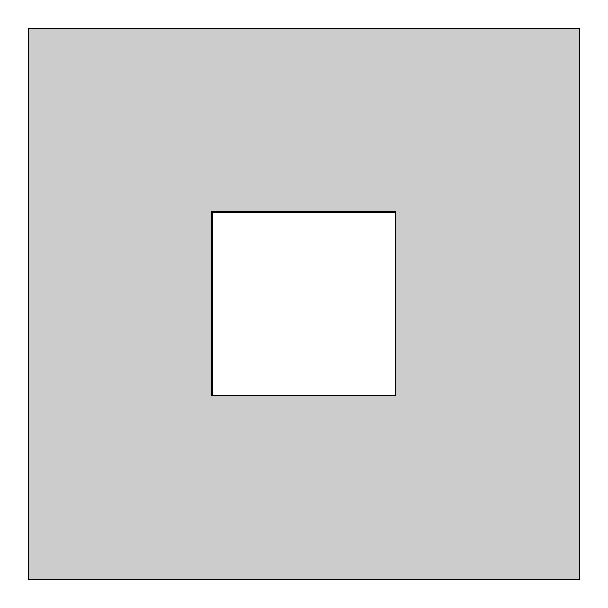
\begin{tikzpicture}
\draw[fill=gray!40] (0,0) rectangle ++(7,7);
\draw[fill=white] (7/3,7/3) rectangle ++(7/3,7/3);
\end{tikzpicture}
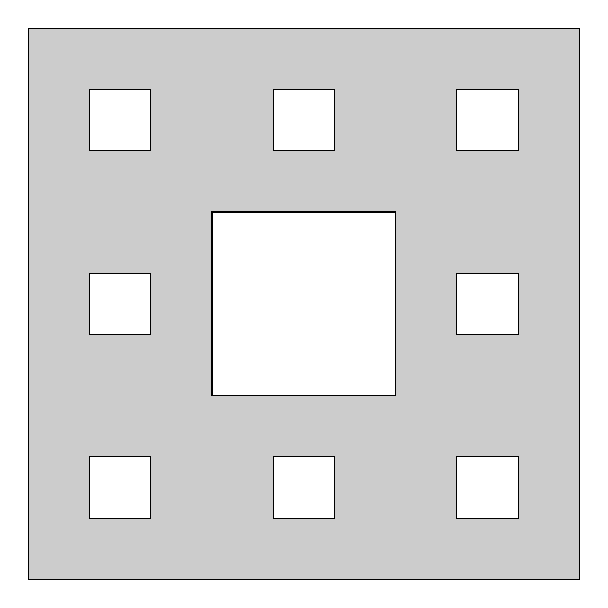
\begin{tikzpicture}
\draw[fill=gray!40] (0,0) rectangle ++(7,7);
\draw[fill=white] (7/3,7/3) rectangle ++(7/3,7/3);
\draw[fill=white] (7/9,7/9) rectangle ++(7/9,7/9);
\draw[fill=white] (28/9,7/9) rectangle ++(7/9,7/9);
\draw[fill=white] (49/9,7/9) rectangle ++(7/9,7/9);
\draw[fill=white] (7/9,28/9) rectangle ++(7/9,7/9);
\draw[fill=white] (7/9,49/9) rectangle ++(7/9,7/9);
\draw[fill=white] (28/9,49/9) rectangle ++(7/9,7/9);
\draw[fill=white] (49/9,49/9) rectangle ++(7/9,7/9);
\draw[fill=white] (49/9,28/9) rectangle ++(7/9,7/9);
\end{tikzpicture}
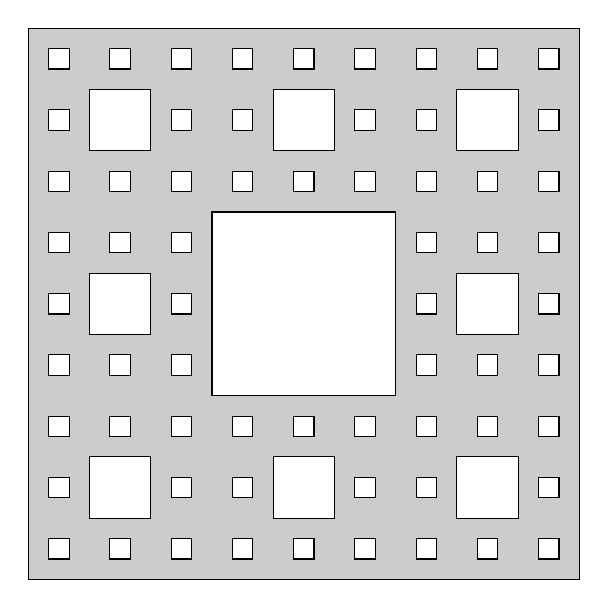
\begin{tikzpicture}
\draw[fill=gray!40] (0,0) rectangle ++(7,7);
\draw[fill=white] (7/3,7/3) rectangle ++(7/3,7/3);
\draw[fill=white] (7/9,7/9) rectangle ++(7/9,7/9);
\draw[fill=white] (7/27,7/27) rectangle ++(7/27,7/27);
\draw[fill=white] (28/27,7/27) rectangle ++(7/27,7/27);
\draw[fill=white] (49/27,7/27) rectangle ++(7/27,7/27);
\draw[fill=white] (7/27,28/27) rectangle ++(7/27,7/27);
\draw[fill=white] (7/27,49/27) rectangle ++(7/27,7/27);
\draw[fill=white] (28/27,49/27) rectangle ++(7/27,7/27);
\draw[fill=white] (49/27,49/27) rectangle ++(7/27,7/27);
\draw[fill=white] (49/27,28/27) rectangle ++(7/27,7/27);
\draw[fill=white] (28/9,7/9) rectangle ++(7/9,7/9);
\draw[fill=white] (70/27,7/27) rectangle ++(7/27,7/27);
\draw[fill=white] (91/27,7/27) rectangle ++(7/27,7/27);
\draw[fill=white] (112/27,7/27) rectangle ++(7/27,7/27);
\draw[fill=white] (70/27,28/27) rectangle ++(7/27,7/27);
\draw[fill=white] (70/27,49/27) rectangle ++(7/27,7/27);
\draw[fill=white] (91/27,49/27) rectangle ++(7/27,7/27);
\draw[fill=white] (112/27,49/27) rectangle ++(7/27,7/27);
\draw[fill=white] (112/27,28/27) rectangle ++(7/27,7/27);
\draw[fill=white] (49/9,7/9) rectangle ++(7/9,7/9);
\draw[fill=white] (133/27,7/27) rectangle ++(7/27,7/27);
\draw[fill=white] (154/27,7/27) rectangle ++(7/27,7/27);
\draw[fill=white] (175/27,7/27) rectangle ++(7/27,7/27);
\draw[fill=white] (133/27,28/27) rectangle ++(7/27,7/27);
\draw[fill=white] (133/27,49/27) rectangle ++(7/27,7/27);
\draw[fill=white] (154/27,49/27) rectangle ++(7/27,7/27);
\draw[fill=white] (175/27,49/27) rectangle ++(7/27,7/27);
\draw[fill=white] (175/27,28/27) rectangle ++(7/27,7/27);
\draw[fill=white] (7/9,28/9) rectangle ++(7/9,7/9);
\draw[fill=white] (7/27,70/27) rectangle ++(7/27,7/27);
\draw[fill=white] (28/27,70/27) rectangle ++(7/27,7/27);
\draw[fill=white] (49/27,70/27) rectangle ++(7/27,7/27);
\draw[fill=white] (7/27,91/27) rectangle ++(7/27,7/27);
\draw[fill=white] (7/27,112/27) rectangle ++(7/27,7/27);
\draw[fill=white] (28/27,112/27) rectangle ++(7/27,7/27);
\draw[fill=white] (49/27,112/27) rectangle ++(7/27,7/27);
\draw[fill=white] (49/27,91/27) rectangle ++(7/27,7/27);
\draw[fill=white] (7/9,49/9) rectangle ++(7/9,7/9);
\draw[fill=white] (7/27,133/27) rectangle ++(7/27,7/27);
\draw[fill=white] (28/27,133/27) rectangle ++(7/27,7/27);
\draw[fill=white] (49/27,133/27) rectangle ++(7/27,7/27);
\draw[fill=white] (7/27,154/27) rectangle ++(7/27,7/27);
\draw[fill=white] (7/27,175/27) rectangle ++(7/27,7/27);
\draw[fill=white] (28/27,175/27) rectangle ++(7/27,7/27);
\draw[fill=white] (49/27,175/27) rectangle ++(7/27,7/27);
\draw[fill=white] (49/27,154/27) rectangle ++(7/27,7/27);
\draw[fill=white] (7/27,133/27) rectangle ++(7/27,7/27);
\draw[fill=white] (28/27,133/27) rectangle ++(7/27,7/27);
\draw[fill=white] (49/27,133/27) rectangle ++(7/27,7/27);
\draw[fill=white] (7/27,154/27) rectangle ++(7/27,7/27);
\draw[fill=white] (7/27,175/27) rectangle ++(7/27,7/27);
\draw[fill=white] (28/27,175/27) rectangle ++(7/27,7/27);
\draw[fill=white] (49/27,175/27) rectangle ++(7/27,7/27);
\draw[fill=white] (49/27,154/27) rectangle ++(7/27,7/27);
\draw[fill=white] (28/9,49/9) rectangle ++(7/9,7/9);
\draw[fill=white] (70/27,133/27) rectangle ++(7/27,7/27);
\draw[fill=white] (91/27,133/27) rectangle ++(7/27,7/27);
\draw[fill=white] (112/27,133/27) rectangle ++(7/27,7/27);
\draw[fill=white] (70/27,154/27) rectangle ++(7/27,7/27);
\draw[fill=white] (70/27,175/27) rectangle ++(7/27,7/27);
\draw[fill=white] (91/27,175/27) rectangle ++(7/27,7/27);
\draw[fill=white] (112/27,175/27) rectangle ++(7/27,7/27);
\draw[fill=white] (112/27,154/27) rectangle ++(7/27,7/27);
\draw[fill=white] (49/9,49/9) rectangle ++(7/9,7/9);
\draw[fill=white] (133/27,133/27) rectangle ++(7/27,7/27);
\draw[fill=white] (154/27,133/27) rectangle ++(7/27,7/27);
\draw[fill=white] (175/27,133/27) rectangle ++(7/27,7/27);
\draw[fill=white] (133/27,154/27) rectangle ++(7/27,7/27);
\draw[fill=white] (133/27,175/27) rectangle ++(7/27,7/27);
\draw[fill=white] (154/27,175/27) rectangle ++(7/27,7/27);
\draw[fill=white] (175/27,175/27) rectangle ++(7/27,7/27);
\draw[fill=white] (175/27,154/27) rectangle ++(7/27,7/27);
\draw[fill=white] (49/9,28/9) rectangle ++(7/9,7/9);
\draw[fill=white] (133/27,70/27) rectangle ++(7/27,7/27);
\draw[fill=white] (154/27,70/27) rectangle ++(7/27,7/27);
\draw[fill=white] (175/27,70/27) rectangle ++(7/27,7/27);
\draw[fill=white] (133/27,91/27) rectangle ++(7/27,7/27);
\draw[fill=white] (133/27,112/27) rectangle ++(7/27,7/27);
\draw[fill=white] (154/27,112/27) rectangle ++(7/27,7/27);
\draw[fill=white] (175/27,112/27) rectangle ++(7/27,7/27);
\draw[fill=white] (175/27,91/27) rectangle ++(7/27,7/27);
\end{tikzpicture}\\
\textbf{Figure 5: First stages in constructing the Sierpinski Carpet $\mathcal{S}$.}
\end{center}
\noindent\fbox{%
	\parbox{\textwidth}{%
		\textbf{Proposition 2.6.3. Results of the Sierpinski Carpet $\mathcal{S}$} \\ The Sierpinski Carpet $\mathcal{S}$,
		\begin{enumerate}[(i)]
			\item has Lebesgue measure 0, i.e. $m(\mathcal{S}) = 0$,
			\item is a Borel set, i.e. $\mathcal{S} \in \mathcal{B}(\mathbb{R}^2)$.
		\end{enumerate}
	}%
}\\\\\\
\textit{Proof.} The idea is similar to the proofs of Proposition 2.6.1 and Proposition 2.6.2.
\begin{enumerate}[(i)]
	\item We take as a fact that, each deletion $D_m$ consists of $8^{m-1}$ disjoint squares, each of area $(\frac{1}{9})^m$. Thus, we can write $\mathcal{S} = A_0 \setminus (\bigcup_{i=1}^{\infty}D_i)$, and by $\sigma$-additivity of $m$, we have that,
	\begin{eqnarray}
	\nonumber
	m(\mathcal{S}) = m(A_0) - \sum_{i=1}^{\infty}m(D_i) = 1 - \sum_{i=1}^{\infty}\frac{8^{i-1}}{9^i} = 1 - \frac{1}{9}\sum_{i=1}^{\infty}\left(\frac{8}{9}\right)^{i-1} = 1 - 1 = 0.
	\end{eqnarray}
	\item Notice that, deletion $D_m \in \mathcal{B}(\mathbb{R}^2), \forall m \geq 1$, since it is a finite union of squares. Moreover, $A_m \in \mathcal{B}(\mathbb{R}^2), \forall m \geq 0$, since $A_0 \in \mathcal{B}(\mathbb{R}^2)$ and $A_m = A_{m-1} \setminus D_m$, so it follows inductively. But, this implies that,
	\begin{eqnarray}
	\nonumber
	\mathcal{S} = \bigcap_{i=0}^{\infty}A_i \in \mathcal{B}(\mathbb{R}^2).
	\end{eqnarray}
\end{enumerate}
${}$ \hfill $\square$ \\\\
Since $\mathcal{S}$ is defined recursively in a consistent procedure, zooming in any particular point of $\mathcal{S}$ still identifies the same carpet structure, so it is self-similar. This notion is prescribed by what is known as a fractal, which has a non-integer dimension. In such cases, the Lebesgue measure $m$ fails to capture a measure for fractal sets, whereas the Hausdorff measure is preferred.
\newpage
\section{Measurable Functions}
This chapter intends to introduce and construct the concept of measurable functions, through a number of important properties and results.
\subsection{Classes of Measurable Functions}
As its name suggests, a measurable function between two measurable spaces preserves the structure of the spaces.\\\\
\noindent\fbox{%
	\parbox{\textwidth}{%
		\textbf{Definition 3.1.1. $\mathcal{F}_1 / \mathcal{F}_2$-Measurable function} \\ Let $(\Omega_1,\mathcal{F}_1)$ and $(\Omega_2,\mathcal{F}_2)$ be measurable spaces. A function $f: \Omega_1 \to \Omega_2$ is called $\mathcal{F}_1/\mathcal{F}_2$-measurable, if the preimage of any $\mathcal{F}_2$-measurable set is $\mathcal{F}_1$-measurable. Alternatively,
		\begin{center}
			$f^{-1}(A) \in \mathcal{F}_1, \ \forall A \in \mathcal{F}_2$,
		\end{center}
		where $f^{-1}(A) := \{\omega_1 \in \Omega_1: f(\omega_1) \in A\}$ is the preimage of $f$.
	}%
}\\\\\\
\textbf{Remark:} It is important to note that the preimage $f^{-1}$ preserves all set operations. This is necessary for proving forthcoming results.\\\\
In a slight abuse of notation, we often drop ‘$\mathcal{F}_1/\mathcal{F}_2$-measurable’ to just ‘measurable’. This definition is a generalisation of particular measurable functions that we usually work with. For instance, a measurable function on a probability space is known as a random variable.\\\\
\noindent\fbox{%
	\parbox{\textwidth}{%
		\textbf{Definition 3.1.2. Random variable $X$} \\ Let $(\Omega_1,\mathcal{F}_1, \mathbb{P})$ be a probability space and $(\Omega_2,\mathcal{F}_2)$ a measurable space. If $X: \Omega_1 \to \Omega_2$ is a measurable function, then it is called a random variable. The probability measure $\mathbb{P}$ on $(\Omega_1,\mathcal{F}_1)$ defines the map,
		\begin{center}
			$\mathbb{P}_X: \mathcal{F}_2 \to [0,1], \ \mathbb{P}_{X}(A) := \mathbb{P}(X^{-1}(A))$,
		\end{center}
		which is called the distribution of $X$.
	}%
}\\\\\\
The distribution of a random variable $X$ seems to be counter-intuitive, but it follows from measurability of $X$, i.e. the preimage of any $\mathcal{F}_2$-measurable set is $\mathcal{F}_1$-measurable (the converse need not be true). In this case, the preimage $X^{-1}: \mathcal{F}_2 \to \mathcal{F}_1$ of $X$ is well-defined on the measurable space $(\Omega_1,\mathcal{F}_1)$, equipped with a probability measure $\mathbb{P}$, and so we can set $\mathbb{P}_X := \mathbb{P} \circ X^{-1}$, where $\mathbb{P}(X \in A) = \mathbb{P}(X^{-1}(A)), \ A \in \mathcal{F}_2$. Summing up, $\mathbb{P}_X$ is a push-forward probability measure on $(\Omega_2,\mathcal{F}_2)$ constructed from $\mathbb{P}$ and $X$.\\\\
\noindent\fbox{%
	\parbox{\textwidth}{%
		\textbf{Definition 3.1.3. Borel function} \\ Let $(\Omega_1,\mathcal{F}_1)$ and $(\Omega_2,\mathcal{F}_2) = (\mathbb{R},\mathcal{B}(\mathbb{R}))$ be measurable spaces. If $X: \Omega_1 \to \mathbb{R}$ is a measurable function, then it is called a Borel function.
	}%
}\\\\\\
\textbf{Remark:} Given measurable spaces $(\Omega_1,\mathcal{F}_1)$ and $(\Omega_2,\mathcal{F}_2)$ that are constructed as in Definition 3.1.2 and Definition 3.1.3, a measurable function $X: \Omega_1 \to \mathbb{R}$ is called a real-valued random variable. The function defined by,
\begin{center}
	$F_X: \mathbb{R} \to [0,1], \ F_X(x) := \mathbb{P}_X((-\infty, x]) = \mathbb{P}(X \leq x)$,
\end{center}
is called the cumulative distribution function (cdf) of $X$, which we analyse later on. The real-valued case is substantially important, as it gives rise to quantities, such as expectation and variance of $X$.\\\\
\textbf{Example 3.1.1.} Let $(\Omega,\mathcal{F})$ be a measurable space and $A \in \mathcal{F}$. We show that the indicator function $\mathds{1}_A : \Omega \to \{0,1\}$ given by,
\begin{center}
$\mathds{1}_A(\omega) =
\begin{cases}
1, & \omega \in A\\
0, & \omega \notin A
\end{cases}$
\end{center}
is $\mathcal{F}/\mathcal{P}(\{0,1\})$-measurable. Then, we have that,
\begin{itemize}
	\item $\mathds{1}_{A}^{-1}(\emptyset) = \emptyset \in \mathcal{F}$,
	\item $\mathds{1}_{A}^{-1}(\{0\}) = A^c \in \mathcal{F}$,
	\item $\mathds{1}_{A}^{-1}(\{1\}) = A \in \mathcal{F}$,
	\item $\mathds{1}_{A}^{-1}(\{0,1\}) = \mathds{1}_A^{-1}(\{0\}) \cup \mathds{1}_A^{-1}(\{1\}) = A^c \cup A = \Omega \in \mathcal{F}$,
\end{itemize}
so $\mathds{1}_A$ is indeed measurable.\\\\
Quite often, it is unhandy to check measurability using the whole target space, in which case the following lemma comes in our aid.\\\\
\noindent\fbox{%
	\parbox{\textwidth}{%
		\textbf{Lemma 3.1.1. Measurability criterion} \\ Let $(\Omega_1,\mathcal{F}_1)$ and $(\Omega_2,\mathcal{F}_2)$ be measurable spaces, where $\mathcal{F}_2 = \sigma(\mathcal{E}), \ \mathcal{E} \subset \mathcal{F}_2$ . Then, $X: \Omega_1 \to \Omega_2$ is a measurable function, if and only if,
		\begin{center}
			$X^{-1}(A) \in \mathcal{F}_1, \ \forall A \in \mathcal{E}$.
		\end{center}
	}%
}\\\\\\
\textit{Proof.} The first direction follows from the definition of measurable functions. Since any $A \in \mathcal{E}$ implies that $A \in \mathcal{F}_2$, then measurability of $X$ gives, $X^{-1}(A) \in \mathcal{F}_1$. Conversely, suppose that $X^{-1}(A) \in \mathcal{F}_1, \ \forall A \in \mathcal{E}$. To prove that $X$ is measurable, it suffices to show that the collection $\mathcal{G} = \{A \subseteq \Omega_2: X^{-1}(A) \in \mathcal{F}_1\}$ is a $\sigma$-algebra on $\Omega_2$, where $\mathcal{E} \subset \mathcal{G}$, so that $\mathcal{F}_2 = \sigma(\mathcal{E}) \subseteq \mathcal{G}$. Then, we observe that,
\begin{enumerate}[(i)]
	\item  $\Omega _1 = X^{-1}(\Omega_2) \in \mathcal{G}$,
	\item $A \in \mathcal{G} \implies B = X^{-1}(A) \in \mathcal{F}_1 \implies B^c = (X^{-1}(A))^c = X^{-1}(A^c) \in \mathcal{F}_1 \implies A^c \in \mathcal{G}$,
	\item $\{A_i\}_{i=1}^{\infty} \subseteq \mathcal{G} \implies B_k = X^{-1}(A_k) \in \mathcal{F}_1, \ \forall k \in \mathbb{N} \\ \implies \bigcup_{i=1}^{\infty}B_i = \bigcup_{i=1}^{\infty}X^{-1}(A_i) = X^{-1}(\bigcup_{i=1}^{\infty}A_i) \in \mathcal{F}_1 \implies \bigcup_{i=1}^{\infty}A_i \in \mathcal{G}$,
\end{enumerate}
so $G$ defines a $\sigma$-algebra on $\Omega_2$. \\ ${}$ \hfill $\square$ \\\\
Recall Example 2.5.1, in which several classes of subsets are $\pi$-systems on $\mathbb{R}$ that generate $\mathcal{B}(\mathbb{R})$. We can apply the above result to conclude that measurability suffices for each such $\pi$-system on $\mathbb{R}$.\\\\
\noindent\fbox{%
	\parbox{\textwidth}{%
		\textbf{Lemma 3.1.2. Equivalent criteria on $\mathbb{R}$} \\ Let $(\Omega,\mathcal{F})$ be a measurable space. The following are equivalent:
		\begin{enumerate}[(a)]
			\item $X: \Omega \to \mathbb{R}$ is a Borel function,
			\item $\{X < a\} \in \mathcal{F}, \ \forall a \in \mathbb{R}$,
			\item $\{X \leq a\} \in \mathcal{F}, \ \forall a \in \mathbb{R}$,
			\item $\{X > a\} \in \mathcal{F}, \ \forall a \in \mathbb{R}$,
			\item $\{X \geq a\} \in \mathcal{F}, \ \forall a \in \mathbb{R}$.
		\end{enumerate}
	}%
}\\\\\\
\textit{Proof.} We show this only for (a) and (b), since the idea is similar for the rest. The first direction is trivial, as in the proof of Lemma 3.1.1. Now, suppose that $X^{-1}((-\infty,a)) = \{X < a\} \in \mathcal{F}, \ \forall a \in \mathbb{R}$. Then, set the class of subsets $\mathcal{E}:=\{(-\infty,a): a \in \mathbb{R}\}$, which is a $\pi$-system on $\mathbb{R}$ that generates $\mathcal{B}(\mathbb{R})$, i.e. $\sigma(\mathcal{E}) = \mathcal{B}(\mathbb{R})$. Hence, by Lemma 3.1.1, we can deduce that $X$ is a Borel function. \\ ${}$ \hfill $\square$
\subsection{Properties of Measurable Functions}
Given a measurable space $(\Omega, \mathcal{F})$, let $X,Y : \Omega \to \mathbb{R}$ be Borel functions. Then, we can also show that, under various operations, measurability is still preserved. For example, \\ $\{X<Y\} = \{\omega \in \Omega: X(\omega) < Y(\omega)\} \in \mathcal{F}$. \\\\
\noindent\fbox{%
	\parbox{\textwidth}{%
		\textbf{Lemma 3.2.1. Sum, Product and Extremum operations on Borel functions} \\ Let $(\Omega,\mathcal{F})$ be a measurable space and $X,Y: \Omega \to \mathbb{R}$ be Borel functions. Then, we have that,
		\begin{enumerate}[(a)]
			\item $\{X < Y\}, \ \{X \leq Y\}, \ \{X=Y\}, \ \{X \neq Y\} \in \mathcal{F}$,
			\item $X+Y, \ X-Y, \ XY$ are Borel functions,
			\item $\max\{X,Y\}, \ \min\{X,Y\}$ are Borel functions.
		\end{enumerate}
	}%
}\\\\\\
\textit{Proof.}
\begin{enumerate}[(a)]
	\item Since $\mathbb{Q}$ is dense in $\mathbb{R}$, i.e. $\overline{\mathbb{Q}} = \mathbb{R}$, then $X <Y$, if $\exists r \in \mathbb{Q}$ such that, $X < r < Y$. Thus, taking the union over all such $r \in \mathbb{Q}$ yields,
	\begin{eqnarray}
	\nonumber
	&&\{X < Y\} = \bigcup_{r\in\mathbb{Q}}(\{X < r < Y\}) = \bigcup_{r\in\mathbb{Q}}(\{X<r\}\cap\{r<Y\}) \in \mathcal{F},
	\end{eqnarray}
	since $\{X<r\},\{r<Y\} \in \mathcal{F}$, by Lemma 3.1.2 (b) and (d). Similarly, we can see that,
	\begin{eqnarray}
	\nonumber
	&&\{X \leq Y\} = \bigcup_{r\in\mathbb{Q}}(\{X \leq r\}\cap\{r \leq Y\}) \in \mathcal{F},\\
	\nonumber
	&{}&\{X=Y\} = \{X \leq Y\} \cap \{X \geq Y\} \in \mathcal{F},\\
	\nonumber
	&{}&\{X \neq Y\} = \{X=Y\}^c \in \mathcal{F}.
	\end{eqnarray}
	\item First, we show that $aX + b, \ a \in \mathbb{R}\setminus\{0\}, \ b \in \mathbb{R}$, is Borel. We have that,
	\begin{eqnarray}
	\nonumber
	&&\{aX+b < c\} = \{aX < c-b\} =
	\begin{cases}
	\{X < \frac{c-b}{a}\}, & a > 0 \\
	\{X > \frac{c-b}{a}\}, & a < 0
	\end{cases}
	\end{eqnarray}
	where $\{X < \frac{c-b}{a}\}, \{X > \frac{c-b}{a}\} \in \mathcal{F}$, by Lemma 3.1.2 (b) and (d). Then, for any $a \in \mathbb{R}$, it follows that,
	\begin{eqnarray}
	\nonumber
	&&\{X+Y < a\} = \{X < a - Y\} \in \mathcal{F},\\
	\nonumber
	&{}& \{X-Y < a\} = \{X < a + Y\} \in \mathcal{F},
	\end{eqnarray}
	since $a - Y$ and $a + Y$ are Borel and by applying property (a). Now, we show that $X^2$ is also Borel. We have that,
	\begin{eqnarray}
	\nonumber
	&&\{X^2 > a\} =
	\begin{cases}
	\Omega, & a < 0\\
	\{X < -\sqrt{a}\} \cup \{X > \sqrt{a}\}, & a \geq 0
	\end{cases}
	\end{eqnarray}
	where $\Omega \in \mathcal{F}$ and $\{X < -\sqrt{a}\} \cup \{X > \sqrt{a}\} \in \mathcal{F}$, by Lemma 3.1.2 (b) and (d). Then, we can write,
	\begin{eqnarray}
	\nonumber
	&& XY = \frac{1}{4}[(X+Y)^2 - (X-Y)^2],
	\end{eqnarray}
	where $(X+Y)^2$ and $(X-Y)^2$ are both Borel, since $X+Y$ and $X-Y$ are, so we can conclude that $XY$ is Borel.
	\item This is quite straightforward. By taking the suitable inequalities for minimum and maximum, for any $a \in \mathbb{R}$, we can see that,
	\begin{eqnarray}
	\nonumber
	&&\{\min\{X,Y\} > a\} = \{X > a\} \cap \{Y > a\} \in \mathcal{F},\\
	\nonumber
	&{}&\{\max\{X,Y\} < a\} = \{X < a\} \cap \{Y < a\} \in \mathcal{F},
	\end{eqnarray}
	since $\{X>a\},\{Y>a\} \in \mathcal{F}$, by Lemma 3.1.2 (d) and $\{X<a\},\{Y<a\} \in \mathcal{F}$, by Lemma 3.1.2 (b).
\end{enumerate}
${}$ \hfill $\square$ \\\\
Interestingly, even limiting operations can maintain measurability.\\\\
\noindent\fbox{%
	\parbox{\textwidth}{%
		\textbf{Lemma 3.2.2. Boundary and Limit operations on Borel functions} \\ Let $(\Omega,\mathcal{F})$ be a measurable space and $(X_n)_{n\geq1}$ be a sequence of Borel functions. Then, we have that,
		\begin{enumerate}[(a)]
			\item $\sup_{n \geq 1}X_n, \ \inf_{n\geq1}X_n$ are Borel functions,
			\item $\limsup_{n\to\infty}X_n, \ \liminf_{n\to\infty}X_n$ are Borel functions.
		\end{enumerate}
	}%
}\\\\\\
\textit{Proof.}
\begin{enumerate}[(a)]
	\item The idea is similar to the proof of part (c) in Lemma 3.2.1. For any $a \in \mathbb{R}$, we can write,
	\begin{eqnarray}
	\nonumber
	&&\left\{\sup_{n \geq 1}X_n < a\right\} = \bigcap_{n=1}^{\infty}\{X_n < a\} \in \mathcal{F},\\
	\nonumber
	&{}&\left\{\inf_{n \geq 1}X_n > a\right\} = \bigcap_{n=1}^{\infty}\{X_n > a\} \in \mathcal{F},
	\end{eqnarray}
	where we used the fact that $\mathcal{F}$ is a $\sigma$-algebra, so it closed under countable intersections.
	\item Using the definition of limit superior and limit inferior,
	\begin{eqnarray}
	\nonumber
	&&\limsup_{n\to\infty}X_n = \adjustlimits\inf_{n \geq 1} \sup_{m \geq n}X_m,\\
	\nonumber
	&{}&\liminf_{n\to\infty}X_n = \adjustlimits\sup_{n \geq 1} \inf_{m \geq n}X_m,
	\end{eqnarray}
	which both are Borel, by applying part (a) twice for each limit.
\end{enumerate}
${}$ \hfill $\square$ \\\\
\noindent\fbox{%
	\parbox{\textwidth}{%
		\textbf{Corollary 3.2.1. Existence of limit on Borel functions} \\ Let $(\Omega,\mathcal{F})$ be a measurable space and $(X_n)_{n\geq1}$ be a sequence of Borel functions. If $\lim_{n\to\infty}X_n$ exists, then
		\begin{eqnarray}
			\nonumber
			&&\lim_{n\to\infty}X_n = \limsup_{n\to\infty}X_n = \liminf_{n\to\infty}X_n,
		\end{eqnarray}
		is a Borel function.
	}%
}\\\\\\
\textit{Proof.} Assuming that the limit of $X_n$ exists, we can write,
\begin{eqnarray}
\nonumber
&&\{-\infty < \lim_{n\to\infty}X_n < +\infty\} = \{\limsup_{n\to\infty}X_n < +\infty\} \cap \{-\infty < \liminf_{n\to\infty}X_n\} \cap \{Y = 0\} \in \mathcal{F},
\end{eqnarray}
since $Y := \limsup_{n\to\infty}X_n - \liminf_{n\to\infty}X_n$ is Borel and by applying Lemma 3.2.2 (b). \\ ${}$ \hfill $\square$ \\\\
Naturally, one can expect from the definition of a measurable function, that a composition of measurable functions is measurable in any general measurable spaces.\\\\
\noindent\fbox{%
	\parbox{\textwidth}{%
		\textbf{Lemma 3.2.3. Composition of measurable functions} \\ Let $(\Omega_1,\mathcal{F}_1)$, $(\Omega_2,\mathcal{F}_2)$ and $(\Omega_3,\mathcal{F}_3)$ be measurable spaces and $f: \Omega_1 \to \Omega_2, \ g: \Omega_2 \to \Omega_3$ be measurable functions. Then, the composition $g \circ f$ is ($\mathcal{F}_1/\mathcal{F}_3$-)measurable.
	}%
}\\\\\\
\textit{Proof.} We prove this through definition chasing. Since $g$ is measurable, $\forall A \in \mathcal{F}_3$, then $g^{-1}(A) \in \mathcal{F}_2$. Now, since $f$ is measurable, then $f^{-1}(g^{-1}(A)) \in \mathcal{F}_1$. But, this implies that,
\begin{center}
	$(g \circ f)^{-1}(A) = f^{-1}(g^{-1}(A)) \in \mathcal{F}_1, \ \forall A \in \mathcal{F}_3$,
\end{center}
so the composition $g \circ f$ is indeed measurable. \\ ${}$ \hfill $\square$ \\\\
Given a target measurable space $(\Omega_2, \mathcal{F}_2)$ and a function $f: \Omega_1 \to \Omega_2$, we can construct a $\sigma$-algebra on $\Omega_1$.\\\\
\noindent\fbox{%
	\parbox{\textwidth}{%
		\textbf{Definition 3.2.1. $\sigma$-Algebra generated by a function $f$} \\ Let $(\Omega_2,\mathcal{F}_2)$ be a measurable space and $f: \Omega_1 \to \Omega_2$ a function, where $\Omega_1$ is a sample space. Then,
		\begin{center}
			$\sigma(f) := \{f^{-1}(A): A \in \mathcal{F}_2\}$,
		\end{center}
		is called the $\sigma$-algebra generated by $f$ on $\Omega_1$.
	}%
}\\\\\\
\textbf{Remarks:}
\begin{enumerate}
	\item We can verify that $\sigma(f)$ defines an algebra on $\Omega_1$, considering that the preimage $f^{-1}$ preserves all set operations.
	\item In fact, $\sigma(f)$ is the smallest $\sigma$-algebra on $\Omega_1$ such that, $f: \Omega_1 \to \Omega_2$ is measurable. In other words, for any $\sigma$-algebra $\mathcal{G}$ on $\Omega_1$ such that $f$ is $\mathcal{G}/\mathcal{F}_2$-measurable, then $\sigma(f) \subseteq \mathcal{G}$.
	\item Given an index set $I$ and a collection $(f_i)_{i \in I}$ of functions $f_i : \Omega_1 \to \Omega_2$, then the $\sigma$-algebra generated by $(f_i)_{i \in I}$ on $\Omega_1$ is defined by, $\sigma(f_i: i \in I) := \sigma(\bigcup_{i \in I}\sigma(f_i))$.
\end{enumerate}
\noindent\fbox{%
	\parbox{\textwidth}{%
		\textbf{Lemma 3.2.4. $\sigma$-Algebra criterion} \\ Let $(\mathbb{R},\mathcal{B}(\mathbb{R}))$ be a measurable space and $X: \Omega \to \mathbb{R}$ a function, where $\Omega$ is a sample space. Then,
		\begin{center}
			$\sigma(X) = \sigma(\{\{X \leq a\}: a \in \mathbb{R}\})$.
		\end{center}
	}%
}\\\\\\
\textit{Proof.} By definition of $\sigma(X)$, notice that $X$ is $\sigma(X)/\mathcal{B}(\mathbb{R})$-measurable, i.e. Borel. Now, by Lemma 3.1.2, $\{X \leq a\} \in \sigma(X), \forall a \in \mathbb{R}$, so $\sigma(\{\{X \leq a\}: a \in \mathbb{R}\}) \subseteq \sigma(X)$. Conversely, by Remark 2, it must be that, $\sigma(X) \subseteq \sigma(\{\{X \leq a\}: a \in \mathbb{R}\})$. \\ ${}$ \hfill $\square$ \\\\
\textbf{Example 3.2.1.} Let $(\Omega,\mathcal{F})$ be a measurable space. Given $A_1, ..., A_n \in \mathcal{F}$ and $b_1, ..., b_n \in \mathbb{R}$, define the function $X: \Omega \to \mathbb{R}$ such that, $X(\omega) := b_1 \mathds{1}_{A_1}(\omega) + ... + b_n \mathds{1}_{A_n}(\omega), \ \omega \in \Omega$. The definition of $\mathds{1}_{A_i}$ is given in Example 3.1.1, $i=1,...,n$. We can check that $X$ is a Borel function, by our results from Lemma 3.2.1. Now, suppose that, $A_i \cap A_j = \emptyset, i \neq j$, and $b_i \neq b_j, i \neq j$. Then, $\sigma(X) = \sigma(\{A_1, ..., A_n\})$. To prove that $\sigma(X) \subseteq \sigma(\{A_1, ..., A_n\})$, it suffices to show that, \\ $\forall a \in \mathbb{R}, \{X \leq a\} \in \sigma(\{A_1,...,A_n\})$, and by Lemma 3.2.4, we can conclude that $\sigma(X) \subseteq \sigma(\{A_1, ..., A_n\})$. We have that,
\begin{eqnarray}
\nonumber
\{X \leq a\} &=& \{b_1 \mathds{1}_{A_1} + ... + b_n \mathds{1}_{A_n} \leq a\}\\
\nonumber
&=& \left\{A_{i_j}: b_{i_j} \leq a, \ i_j \in \{1,...,n\}, \ j = 1,...,m\right\}\\
\nonumber
&=& \bigcup_{j=1}^{m}A_{i_{j}} \in \sigma(\{A_1,...,A_n\}),
\end{eqnarray}
which follows by construction of $X$. Conversely, to show that $\{A_1, ..., A_n\} \subset \sigma(X)$, observe that,
\begin{center}
	$\{X = b_i\} = A_i \in \sigma(X), \ i = 1, ..., n$,
\end{center}
and so $\sigma(\{A_1, ..., A_n\}) \subseteq \sigma(X)$.
\begin{center}
	\noindent\rule{12cm}{0.4pt}
\end{center}
\textbf{Exercise 3.2.1.} Let $([0,1], \mathcal{B}([0,1]))$ be a measurable space and given a sample space $\Omega_2$, define the functions $X: [0,1] \to \Omega_2$, $Y: [0,1] \to \{0,1\}$ by,
\begin{center}
$X(\omega) =
\begin{cases}
A_1, & \omega \in [0, \frac{1}{4}]\\
A_2, & \omega \in (\frac{1}{4}, \frac{1}{2}]\\
A_3, & \omega \in (\frac{1}{2},1]
\end{cases}$
\ \ \ , \ \ \
$Y(\omega) = 
\begin{cases}
0, & \omega \in [0,\frac{1}{2}]\\
1, & \omega \in (\frac{1}{2},1]
\end{cases}$ \ \ \ .
\end{center}
Find $\sigma(X)$ and check that, $\sigma(Y) \subset \sigma(X)$. \\\\
\textit{Solution.} First, observe that the target spaces of $X$ and $Y$ differ, but the sigma algebras generated by $X$ and $Y$ are both defined on $[0,1]$. Then, we can easily compute that $\sigma(X)$ and $\sigma(Y)$ are given by,
\begin{eqnarray}
	\nonumber
	&&\sigma(X) = \left\{\emptyset, \left[0,\frac{1}{4}\right], \left(\frac{1}{4},\frac{1}{2}\right], \left(\frac{1}{2},1\right], \left[0,\frac{1}{2}\right], \left(\frac{1}{4},1\right], \left[0,\frac{1}{4}\right] \cup \left(\frac{1}{2},1\right], [0,1]\right\},\\
	\nonumber
	&{}&\sigma(Y) = \left\{\emptyset, \left[0,\frac{1}{2}\right], \left(\frac{1}{2},1\right], [0,1]\right\},
\end{eqnarray}
where $\sigma(Y) \subset \sigma(X)$ is verified.
\begin{center}
	\noindent\rule{12cm}{0.4pt}
\end{center}
\newpage
\section{Integration}
In Real Analysis, we introduce the Riemann Integral, which approximates the area under a curve in a given interval via vertical rectangles and considering a sequence of step functions that converges to the associated curve. However, under ‘rough’ functions, Riemann Integration fails to analyse sequences of functions when taking limits. In contrast, the Lebesgue Integral considers horizontal shapes, which are not necessarily rectangles, so it is more flexible. It is also more descriptive as to when it is possible to take limits, by the so-called Monotone-Convergence Theorem, which we review onwards. The road map begins from defining the integral for non-negative simple functions, then approximate non-negative Borel functions and hence for general Borel functions. Thereby, we study relationships between measures and modes of convergence.
\subsection{Integral of non-negative Simple Functions}
Let $\Omega=[0,1]$ be a sample space and consider the indicator function $\mathds{1}_{\mathbb{Q}}: [0,1] \to \mathbb{R}$ on the rational numbers $\mathbb{Q}$ by,
\begin{center}
$\mathds{1}_{\mathbb{Q}}(\omega) =
\begin{cases}
1, & \omega \in \mathbb{Q}\\
0, & \omega \in \mathbb{R}\setminus\mathbb{Q}
\end{cases}$
\end{center}
Since $\mathbb{Q}$ and $\mathbb{R}\setminus\mathbb{Q}$ are both dense in $\mathbb{R}$, any partition of $[0,1]$ has both rational and irrational numbers in any sub-interval, so there is no step function converging to $\mathds{1}_{\mathbb{Q}}$. Hence, it is not Riemann integrable. However, consider the integral,
\begin{eqnarray}
\nonumber
\int_{0}^{1}\mathds{1}_{\mathbb{Q}}(x)dx = 1 \times m(\mathds{1}_{\mathbb{Q}}^{-1}(1)) + 0 \times m(\mathds{1}_{\mathbb{Q}}^{-1}(0)) = m(\mathbb{Q}\cap[0,1]) = 0,
\end{eqnarray}
since $Q\cap[0,1]$ is a countable set, so the Lebesgue measure $m$ assigns a value of $0$. This is precisely the Lebesgue integral of the indicator function $\mathds{1}_{\mathbb{Q}}$. \\\\
\noindent\fbox{%
	\parbox{\textwidth}{%
		\textbf{Definition 4.1.1. Integral of $\mathds{1}_A$ with respect to $\mu$} \\ Let $(\Omega, \mathcal{F}, \mu)$ be a measure space and $\mathds{1}_A: \Omega \to \mathbb{R}$ the indicator function of $A \in \mathcal{F}$. Then,
		\begin{center}
			$\int_\Omega \mathds{1}_A d\mu := \mu(A)$,
		\end{center}
		is called the integral of $\mathds{1}_A$ with respect to $\mu$.
	}%
}\\\\\\
We need to include a particular set of measurable functions, which are introduced in Example 3.2.1, and are critical to define the integral on measurable functions.\\\\
\noindent\fbox{%
	\parbox{\textwidth}{%
		\textbf{Definition 4.1.2. Non-negative Simple function $f$ and its integral with respect to $\mu$} \\ Let $(\Omega, \mathcal{F}, \mu)$ be a measure space. A function $f: \Omega \to \mathbb{R}$ is called a non-negative simple function, if $\exists \ a_i \geq 0$ and $A_i \in \mathcal{F}, \ i = 1,...,n$, with $A_i \cap A_j = \emptyset, \ i \neq j$, such that,
		\begin{center}
			$f(\omega) = \sum_{i=1}^{n}a_i\mathds{1}_{A_i}(\omega), \ \forall \omega \in \Omega$.
		\end{center}
		The integral of $f$ with respect to $\mu$ is defined by,
		\begin{center}
			$\int_\Omega f d\mu := \sum_{i=1}^{n}a_i\mu(A_i)$.
		\end{center}
	}%
}\\\\\\
\textbf{Remarks:}
\begin{enumerate}
	\item We specifically introduce the non-negative case, as it is the first stepping stone in reaching the integral.
	\item Representation is not unique, but the integral agrees nevertheless.
	\item Given a measure space $(\Omega,\mathcal{F},\mu)$, it can be verified that, if $f, g$ are non-negative simple functions, then $f+g, \ fg, \ \min\{f,g\}, \ \max\{f,g\}$ are also non-negative simple functions.
\end{enumerate}
Primary desirable integral properties of non-negative simple functions arise.\\\\
\noindent\fbox{%
	\parbox{\textwidth}{%
		\textbf{Proposition 4.1.1. Integral properties with respect to $\mu$ of non-negative simple functions} \\ Let $(\Omega, \mathcal{F}, \mu)$ be a measure space and $f,g: \Omega \to \mathbb{R}$ non-negative simple functions. Then, we have the following properties:
		\begin{enumerate}[(a)]
			\item \textit{Linearity:} $\int_\Omega (\alpha f + \beta g) d\mu = \alpha\int_\Omega f d\mu + \beta\int_\Omega g d\mu, \ \forall \alpha,\beta \geq 0$,
			\item \textit{Monotonicity:} If $f(\omega) \leq g(\omega), \forall \omega \in \Omega$, then $\int_\Omega f d\mu \leq \int_\Omega g d\mu$.
			\item \textit{Measurability:} $\nu(A) := \int_\Omega f \mathds{1}_A d\mu, \ \forall A \in \mathcal{F}$, defines a measure on $(\Omega, \mathcal{F})$.
		\end{enumerate}
	}%
}\\\\\\
\textit{Proof.} Checking that linearity and monotonicity hold involves messy computations with no substantial point, so we skip it and prove measurability. Recall that $\nu$ is a measure on $(\Omega,\mathcal{F})$, if it is $\sigma$-additive and the empty set has $\nu$ measure $0$. Since $f$ is non-negative simple function, we can write, $f(\omega) = \sum_{i=1}^{n}a_i \mathds{1}_{A_i}(\omega), \forall \omega \in \Omega$, where $a_i \geq 0$ and $A_i \in \mathcal{F}, i = 1,...,n$, with $A_i \cap A_j = \emptyset$. Then, we have that,
\begin{enumerate}
	\item $\nu(\emptyset) = \int_\Omega f \mathds{1}_\emptyset d\mu = \int_\Omega 0 d\mu = 0$.
	\item Let $\{E_j\}_{j=1}^{\infty} \subseteq \mathcal{F}$, where $E_k$ are disjoint, $\forall k \in \mathbb{N}$, and set $E := \bigcup_{j=1}^{\infty}E_j$. It follows that,
	\begin{eqnarray}
	\nonumber
	\nu(E) &=& \int_\Omega f \mathds{1}_E d\mu\\
	\nonumber
	&=& \sum_{i=1}^{n}a_i \int_\Omega \mathds{1}_{A_i \cap E} d\mu \ \ \ \ \ \text{($\mathds{1}_{A_i}\mathds{1}_E = \mathds{1}_{A_i \cap E}$)} \\
	\nonumber
	&=& \sum_{i=1}^{n}a_i \mu(A_i \cap E) \ \ \ \ \ \text{(integral of indicator function)} \\
	\nonumber
	&=& \sum_{i=1}^{n}a_i \mu\left(\bigcup_{j=1}^{\infty}(A_i \cap E_j)\right) \\
	\nonumber
	&=& \sum_{j=1}^{\infty}\sum_{i=1}^{n}a_i \mu(A_i \cap E_j) \ \ \ \ \ \text{($\sigma$-additivity of $\mu$)} \\
	\nonumber
	&=& \sum_{j=1}^{\infty}\int_\Omega \sum_{i=1}^{n}a_i \mathds{1}_{A_i}\mathds{1}_{E_j} d\mu \ \ \ \ \ \text{(integral of non-negative simple function)} \\
	\nonumber
	&=& \sum_{j=1}^{\infty}\int_\Omega f \mathds{1}_{E_j} d\mu \\
	\nonumber
	&=& \sum_{j=1}^{\infty}\nu(E_j).
	\end{eqnarray}
\end{enumerate}
${}$ \hfill $\square$\\\\
\textbf{Remark:} Given a measure space $(\Omega,\mathcal{F},\mu)$ and $A \in \mathcal{F}$, if $f$ is a non-negative simple function, then we can write,
\begin{center}
	$\int_\Omega f \mathds{1}_A d\mu = \int_A f d\mu$.
\end{center}
In fact, this holds for any Borel function $f:\Omega\to\mathbb{R}$.\\\\
Since the integral of a non-negative simple function defines a measure on a given measurable space, the following property is immediate.\\\\
\noindent\fbox{%
	\parbox{\textwidth}{%
		\textbf{Corollary 4.1.1. Integral Continuity from below of non-negative simple functions} \\ Let $(\Omega, \mathcal{F}, \mu)$ be a measure space and $f:\Omega\to\mathbb{R}$ a non-negative simple function. If $\{E_i\}_{i=1}^{\infty} \subseteq \mathcal{F},\\ E_k \subseteq E_{k+1}, \forall k \in \mathbb{N}$, then
		\begin{center}
			$\lim_{n\to\infty}\int_{E_n} f d\mu = \int_E f d\mu$,
		\end{center}
	where $E := \bigcup_{i=1}^{\infty}E_i$.
	}%
}
\subsection{Approximation of non-negative Borel functions}
Let $(\Omega,\mathcal{F},\mu)$ be a measure space and $f: \Omega \to \mathbb{R}_+$ a non-negative Borel function. Consider the sequence of non-negative simple functions $(f_i)_{i\geq1}$ given by,
\begin{center}
	$f_i(\omega) = \sum_{k=1}^{2^{2i}}\frac{k-1}{2^i}\mathds{1}_{\{\frac{k-1}{2^i} \leq f < \frac{k}{2^i}\}}(\omega) + 2^i \mathds{1}_{\{2^i \leq f\}}(\omega), \ \forall \omega \in \Omega$.
\end{center}
In particular, for each $i \geq 1$, the range of $f$ is divided into $2^{2i} + 1$ intervals, each of length $2^{-i}$. Then, $(f_i)_{i\geq1}$ is an increasing sequence, which converges pointwise to $f$, i.e. $\sup_{i\geq1}f_i = f$. Intuitively, $f$ is approximated from below and as $i$ gets larger, both the sub-intervals increase and the length of each decreases, exponentially. An example of a non-negative Borel function $f:\mathbb{R}_+ \to \mathbb{R}_+$ is illustrated in Figure 6 below.
\begin{center}
\begin{tikzpicture}[x=1.2cm, y=1.2cm]
\begin{axis}[
	axis lines = left,
	xlabel = {$x = f^{-1}(f(x))$},
	xmin=0,xmax=2.5,
	ymin=0, ymax=5,
	ytick={2,4},
	xticklabels = empty,
	yticklabels = {$2 = 2^1$, $4 = 2^2$},
	]
	\addplot [
	domain=0:2,
	samples=100, 
	]
	{-x^2 + 4};
	\node at (1.5,2.625) {$f(x)$};
	\addplot[gray!50] coordinates {(0,2) (2^(0.5),2) (2^(0.5),1.5) ((2.5)^(0.5),1.5) ((2.5)^(0.5),1) (3^(0.5),1) (3^(0.5),0.5) ((3.5)^(0.5),0.5) ((3.5)^(0.5),0) (2,0)};
	\node[gray!50] at (0.75,2.25) {$f_1(x)$};
	\addplot[gray!80] coordinates {(0,4) (0,15/4) ((1/4)^(1/2),15/4) ((1/4)^(1/2),14/4) ((2/4)^(1/2),14/4) ((2/4)^(1/2),13/4) ((3/4)^(1/2),13/4) ((3/4)^(1/2),12/4) ((4/4)^(1/2),12/4) ((4/4)^(1/2),11/4) ((5/4)^(1/2),11/4) ((5/4)^(1/2),10/4) ((6/4)^(1/2),10/4) ((6/4)^(1/2),9/4) ((7/4)^(1/2),9/4) ((7/4)^(1/2),8/4) ((8/4)^(1/2),8/4) ((8/4)^(1/2),7/4) ((9/4)^(1/2),7/4) ((9/4)^(1/2),6/4) ((10/4)^(1/2),6/4) ((10/4)^(1/2),5/4) ((11/4)^(1/2),5/4) ((11/4)^(1/2),4/4) ((12/4)^(1/2),4/4) ((12/4)^(1/2),3/4) ((13/4)^(1/2),3/4) ((13/4)^(1/2),2/4) ((14/4)^(1/2),2/4) ((14/4)^(1/2),1/4) ((15/4)^(1/2),1/4) ((15/4)^(1/2),0) ((16/4)^(1/2),0)};
	\node[gray!80] at (0.75,3) {$f_2(x)$};
\end{axis}
\end{tikzpicture}\\
\textbf{Figure 6: Approximation of Borel function $f: \mathbb{R}_+ \to \mathbb{R}_+$ by $f_1$ and $f_2$.}
\end{center}
Given a measure space $(\Omega, \mathcal{F},\mu)$, we can now define the integral of a non-negative Borel function.\\\\
\noindent\fbox{%
	\parbox{\textwidth}{%
		\textbf{Definition 4.2.1. Integral with respect to $\mu$ of non-negative Borel function $f$} \\ Let $(\Omega, \mathcal{F}, \mu)$ be a measure space and $f = \sup_{i\geq1}f_i$ a non-negative Borel function, where $(f_i)_{i\geq1}$ is an increasing sequence of non-negative simple functions associated with $f$. Then, the integral of $f$ with respect to $\mu$ is defined by,
		\begin{center}
			$\int_\Omega f d\mu := \sup_{i\geq1} \int_\Omega f_i d\mu = \lim_{i\to\infty} \int_\Omega f_i d\mu$.
		\end{center} 
	}%
}\\
Note that the integral of $f$ with respect to $\mu$ can diverge. Some questions to ask concern whether the limiting integrals of distinct sequences of simple functions $(f_i)_{i\geq1}, \ (g_i)_{i\geq1}$ converging pointwise to $f$ agree. To check this, we first state the fundamental Monotone-Convergence theorem.\\\\
\noindent\fbox{%
	\parbox{\textwidth}{%
		\textbf{Theorem 4.2.1. Monotone-Convergence Theorem} \\ Let $(\Omega, \mathcal{F}, \mu)$ be a measure space. If $(f_i)_{i\geq1}$ is an increasing sequence of non-negative Borel functions, then
		\begin{center}
			$\lim_{i\to\infty} \int_\Omega f_i d\mu = \int_\Omega \lim_{i\to\infty} f_i d\mu$.
		\end{center} 
	}%
}\\\\\\
The idea of this result is closely related to the monotonicity properties of measures. As an application, we answer our previous concern. Given a measure space $(\Omega,\mathcal{F},\mu)$, let $(f_i)_{i\geq1}$ and $(g_i)_{i\geq1}$ be distinct increasing sequences of non-negative simple functions converging pointwise to a Borel function $f:\Omega\to\mathbb{R}_+$, i.e. $f = \sup_{i\geq1}f_i = \sup_{i\geq1}g_i$. Since $(g_i)_{i\geq1}$ is increasing, this implies that,
\begin{eqnarray}
	\nonumber
	g_j \leq \sup_{i \geq 1}f_i = f, \forall j \geq 1 \implies \int_\Omega g_j d\mu \leq \int_\Omega \sup_{i \geq 1}f_i d\mu = \sup_{i \geq 1} \int_\Omega f_i d\mu,
\end{eqnarray}
which follows by Proposition 4.1.1 (b) and the latter equality by the Monotone-Convergence Theorem. Now, taking supremum over $g_j$ yields,
\begin{eqnarray}
\nonumber
\sup_{j \geq 1} \int_\Omega g_j d\mu \leq \sup_{i \geq 1} \int_\Omega f_i d\mu.
\end{eqnarray}
By symmetry of the argument, we can deduce that the reversed inequality also holds, so that indeed,
\begin{eqnarray}
\nonumber
\sup_{j \geq 1} \int_\Omega g_j d\mu = \sup_{i \geq 1} \int_\Omega f_i d\mu.
\end{eqnarray}
\textit{Proof of Theorem 4.2.1.} Let $f$ be the pointwise limit of $(f_i)_{i\geq1}$, i.e. $f := \sup_{i\geq1}f_i = \lim_{i\to\infty}f_i$, which is Borel by Lemma 3.2.2. Since $f_i \leq f, \forall i \geq 1$, by applying Proposition 4.1.1 (b), we get that,
\begin{eqnarray}
\nonumber
\int_\Omega f_i d\mu \leq \int_\Omega f d\mu \implies \lim_{i\to\infty} \int_\Omega f_i d\mu \leq \int_\Omega f d\mu,
\end{eqnarray}
where we take the limit as $i \to \infty$. To prove the reversed inequality, $f$ is non-negative Borel, so we consider a sequence $(\phi_n)_{n\geq1}$ of non-negative simple functions that converges pointwise to $f$, i.e. $f = \sup_{n\geq1}\phi_n = \lim_{n\to\infty}\phi_n$. Given $n \geq 1$ and $\alpha \in (0,1)$, define the sets,
\begin{center}
	$A_i := \{f_i \geq \alpha\phi_n\} \in \mathcal{F}, \ i\geq1$,
\end{center}
in which case $A_k \subseteq A_{k+1}, \forall k \in \mathbb{N}$. Then, we can write,
\begin{eqnarray}
\nonumber
\bigcup_{i=1}^{\infty}A_i &=& \{\exists j \geq 1 \ \text{such that} \ f_j \geq \alpha\phi_n \}\\
\nonumber
&=& \{\sup_{j \geq 1}f_j \geq \alpha\phi_n\}\\
\nonumber
&=& \{f \geq \alpha\phi_n\} = \Omega,
\end{eqnarray}
which in turn implies that,
\begin{eqnarray}
\nonumber
\int_\Omega f_i d\mu \geq \alpha\int_{A_i} \phi_n d\mu \xrightarrow{i \to \infty} \lim_{i\to\infty} \int_\Omega f_i d\mu \geq \alpha\int_\Omega \phi_n d\mu,
\end{eqnarray}
where $\alpha$ can be taken outside the integral by Proposition 4.1.1 (a). It only remains to take limits as $n \to \infty$ and $\alpha \to 1$, so that,
\begin{eqnarray}
\nonumber
\lim_{i \to \infty} \int_\Omega f_i d\mu \geq \int_\Omega f d\mu.
\end{eqnarray}
${}$ \hfill $\square$
\subsection{Integral of Borel Functions}
Defining the integral of any Borel function $f: \Omega \to \mathbb{R}$ in a measure space $(\Omega,\mathcal{F},\mu)$ requires consideration of the negative part of $f$. As we know how to approximate a non-negative Borel function, we seperate $f$ by,
\begin{center}
	$f^+(\omega) := \max\{0,f(\omega)\}$ and $f^-(\omega) := \max\{0,-f(\omega)\}, \ \forall \omega \in \Omega$.
\end{center}
Observe that both $f^+$ and $f^-$ are non-negative Borel functions, and we can write,
\begin{center}
$f(\omega) = f^+(\omega) - f^-(\omega), \ \forall \omega \in \Omega$.
\end{center}
Figure 7 depicts the meaning of splitting a Borel function, by identifying the positive and negative range of $f$, so as to construct the associated non-negative Borel functions, which we know how to integrate.
\begin{center}
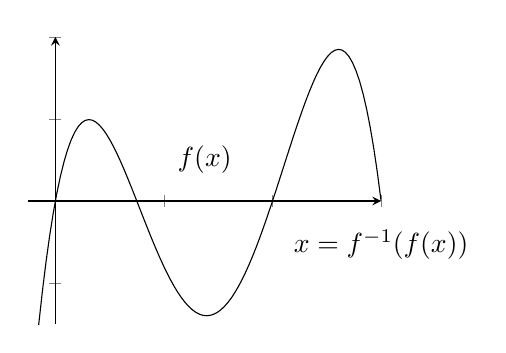
\begin{tikzpicture}
\begin{axis}[
width=0.5\textwidth,
axis lines = middle,
x label style={at={(current axis.right of origin)},anchor=north, below=2.5mm},
xlabel = {$x = f^{-1}(f(x))$},
xmin=-0.5,xmax=6,
ymin=-15,ymax=20,
yticklabels=\empty,
xticklabels=\empty,
]
\node at (2.75,5) {$f(x)$};
\addplot[domain=-0.5:6,samples=100] {-1*x*(x-1.5)*(x-4)*(x-6)};
\end{axis}
\end{tikzpicture}
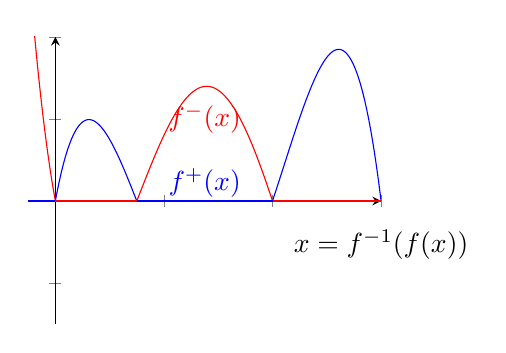
\begin{tikzpicture}
\begin{axis}[
	width=0.5\textwidth,
	axis lines = middle,
	x label style={at={(current axis.right of origin)},anchor=north, below=2.5mm},
	xlabel = {$x = f^{-1}(f(x))$},
	xmin=-0.5,xmax=6,
	ymin=-15,ymax=20,
	yticklabels=\empty,
	xticklabels=\empty,
	]
	\node[red] at (2.75,10) {$f^-(x)$};
	\node[blue] at (2.75,2.25) {$f^+(x)$};
	\addplot[color=blue, domain=0:1.5,samples=100] {-1*x*(x-1.5)*(x-4)*(x-6)};
	\addplot[color=blue, domain=4:6,samples=100] {-1*x*(x-1.5)*(x-4)*(x-6)};
	\addplot[color=red, domain=-0.5:0,samples=100] {1*x*(x-1.5)*(x-4)*(x-6)};
	\addplot[color=red, domain=1.5:4,samples=100] {1*x*(x-1.5)*(x-4)*(x-6)};
	\addplot[color=blue, domain=-0.5:0,samples=100] {0};
	\addplot[color=blue, domain=1.5:4,samples=100] {0};
	\addplot[color=red, domain=0:1.5,samples=100] {0};
	\addplot[color=red, domain=4:6,samples=100] {0};
\end{axis}
\end{tikzpicture}\\
\textbf{Figure 7: Separation of Borel function $f:\mathbb{R}\to\mathbb{R}$ by $f^+$ and $f^-$}.
\end{center}
\noindent\fbox{%
	\parbox{\textwidth}{%
		\textbf{Definition 4.3.1. Integral with respect to $\mu$ of Borel function $f$} \\ Let $(\Omega, \mathcal{F}, \mu)$ be a measure space and $f:\Omega\to\mathbb{R}$ a Borel function. Then, we say that $f$ is $\mu$-integrable, if
		\begin{center}
			$\int_\Omega f^+ d\mu < \infty$ \ and \ $\int_\Omega f^- d\mu < \infty$.
		\end{center}
		Then, the integral of $f$ with respect to $\mu$ is defined by,
		\begin{center}
			$\int_\Omega f d\mu := \int_\Omega f^+ d\mu - \int_\Omega f^- d\mu$.
		\end{center}
	}%
}\\\\\\
\textbf{Remark:} In the case where we have a probability space $(\Omega,\mathcal{F},\mathbb{P})$ and $X:\Omega\to\mathbb{R}$ a real-valued random variable, which is $\mathbb{P}$-integrable, then the integral of $X$ with respect to $\mathbb{P}$ is well-defined and is known as the expectation of $X$, i.e.
\begin{center}
	$\mathbb{E}^{\mathbb{P}}[X] := \int_\Omega X d\mathbb{P}$.
\end{center}
As for non-negative simple functions, we have the equivalent integral properties for Borel functions.\\\\
\noindent\fbox{%
	\parbox{\textwidth}{%
		\textbf{Proposition 4.3.1. Integral properties with respect to $\mu$ of Borel functions} \\ Let $(\Omega, \mathcal{F}, \mu)$ be a measure space and $f,g: \Omega \to \mathbb{R}$ Borel functions. Then, we have the following properties:
		\begin{enumerate}[(a)]
			\item \textit{Linearity:} $\int_\Omega (\alpha f + \beta g) d\mu = \alpha\int_\Omega f d\mu + \beta\int_\Omega g d\mu, \ \forall \alpha,\beta \in \mathbb{R}$,
			\item \textit{Monotonicity:} If $f(\omega) \leq g(\omega), \forall \omega \in \Omega$, then $\int_\Omega f d\mu \leq \int_\Omega g d\mu$.
			\item \textit{Measurability:}  If $f(\omega) \geq 0, \forall \omega\in\Omega$, then $\nu(A) := \int_\Omega f\mathds{1}_A d\mu, \ \forall A \in \mathcal{F}$, defines a measure on $(\Omega, \mathcal{F})$.
		\end{enumerate}
	}%
}\\
\textit{Proof.} Proving (a) and (b) comes from splitting $f$ and $g$ into non-negative Borel functions and with the use of the Monotonone-Convergence theorem and Proposition 4.1.1 (a) and (b).
\begin{enumerate}[(a)]
	\item Write $f = f^+ - f^-$, \ $g = g^+ - g^-$, and consider the sequences of non-negative simple functions $(f_i^+)_{i\geq1}, \ (f_i^-)_{i\geq1}, \ (g_i^+)_{i\geq1}, \ (g_i^-)_{i\geq1}$ such that, $f^+ = \lim_{i\to\infty}f_i^+, \ f^- = \lim_{i\to\infty}f_i^-, \ g^+ = \lim_{i\to\infty}g_i^+, \ g^- = \lim_{i\to\infty}g_i^-$. Observe that, $\forall \alpha, \beta \in \mathbb{R}$, $(\alpha f + \beta g)^+ = \alpha f^+ + \beta g^+$ and $(\alpha f + \beta g)^- = \alpha f^- + \beta g^-$. Then, it follows that,
	\begin{eqnarray}
	\nonumber
	\int_\Omega (\alpha f + \beta g) d\mu &=& \int_\Omega (\alpha f^+ + \beta g^+)d\mu - \int_\Omega (\alpha f^- + \beta g^-)d\mu \ \ \ \ \ \text{(by Definition 4.3.1)}\\
	\nonumber
	&=& \int_\Omega \lim_{i\to\infty}(\alpha f_i^+ + \beta g_i^+)d\mu - \int_\Omega \lim_{i\to\infty} (\alpha f_i^- + \beta g_i^-)d\mu\\
	\nonumber
	&=& \lim_{i\to\infty}\int_\Omega (\alpha f_i^+ + \beta g_i^+)d\mu - \lim_{i\to\infty}\int_\Omega (\alpha f_i^- + \beta g_i^-)d\mu \ \ \ \ \ \text{(by Theorem 4.2.1)}\\
	\nonumber
	&=& \lim_{i\to\infty}\left(\alpha\int_\Omega f_i^+ d\mu + \beta\int_\Omega g_i^+ d\mu\right) - \lim_{i\to\infty}\left(\alpha\int_\Omega f_i^- d\mu + \beta\int_\Omega g_i^- d\mu\right) \\
	\nonumber
	&{}& \text{(by Proposition 4.1.1 (a))}\\
	\nonumber
	&=& \left(\alpha\int_\Omega f^+ d\mu + \beta\int_\Omega g^+ d\mu\right) - \left(\alpha\int_\Omega f^- d\mu + \beta\int_\Omega g^- d\mu\right) \\
	\nonumber
	&{}& \text{(again by Theorem 4.2.1)}\\
	\nonumber
	&=& \alpha\int_\Omega f d\mu + \beta\int_\Omega g d\mu.
	\end{eqnarray}
	\item With the same settings as in (a), if $f \leq g$, then $f^+ \leq g^+$ and $f^- \geq g^-$. This in turn implies that, $f_i^+ \leq g_i^+$ and $f_i^- \geq g_i^-$, $\forall i \geq 1$, by construction of approximating non-negative simple functions. Now, we get that,
	\begin{eqnarray}
	\nonumber
	\int_\Omega f d\mu &=& \int_\Omega f^+ d\mu - \int_\Omega f^- d\mu\\
	\nonumber
	&=& \int_\Omega (f^+ - f^-) d\mu \ \ \ \ \ \text{(by part (a))}\\
	\nonumber
	&=& \int_\Omega\lim_{i\to\infty} (f_i^+ - f_i^-)d\mu\\
	\nonumber
	&=& \lim_{i\to\infty}\int_\Omega (f_i^+ - f_i^-)d\mu \ \ \ \ \ \text{(by Theorem 4.2.1)}\\
	\nonumber
	&\leq& \lim_{i\to\infty}\int_\Omega (g_i^+ - g_i^-)d\mu \ \ \ \ \ \text{(by Proposition 4.1.1 (b))}\\
	\nonumber
	&=& \int_\Omega\lim_{i\to\infty} (g_i^+ - g_i^-)d\mu \ \ \ \ \ \text{(again by Theorem 4.2.1)}\\
	\nonumber
	&=& \int_\Omega\lim_{i\to\infty} g_i^+ d\mu - \int_\Omega\lim_{i\to\infty} g_i^- d\mu \ \ \ \ \ \text{(again by part (a))}\\
	\nonumber
	&=& \int_\Omega g d\mu,
	\end{eqnarray}
	where we used the fact that, $f_i^+ - f_i^- \leq g_i^+ - g_i^-, \ \forall i \geq 1$.
	\item We need to show that $\nu$ is $\sigma$-additive and the empty set has $\nu$ measure $0$. Then, we have that,
	\begin{enumerate}[1.]
		\item $\nu(\emptyset) = \int_\Omega f \mathds{1}_\emptyset d\mu = \int_\Omega 0 d\mu = 0$.
		\item Let $\{E_j\}_{j=1}^{\infty} \subseteq \mathcal{F}$, where $E_k$ are disjoint, $\forall k \in \mathbb{N}$, and set $E := \bigcup_{j=1}^{\infty}E_j$. It follows that,
		\begin{eqnarray}
		\nonumber
		\nu(E) &=& \int_\Omega f \mathds{1}_E d\mu\\
		\nonumber
		&=& \int_\Omega f \mathds{1}_{\bigcup_{j=1}^{\infty}E_j} d\mu\\
		\nonumber
		&=& \int_\Omega \lim_{n\to\infty} f\mathds{1}_{\bigcup_{j=1}^{n}E_j} d\mu \ \ \ \ \ \text{(since $f\mathds{1}_{\bigcup_{j=1}^{k}E_j} \subseteq f\mathds{1}_{\bigcup_{j=1}^{k+1}E_j}, \ \forall k \in \mathbb{N}$)}\\
		\nonumber
		&=& \lim_{n\to\infty}\int_\Omega f\mathds{1}_{\bigcup_{j=1}^{n}E_j} d\mu \ \ \ \ \ \text{(by Theorem 4.2.1)}\\
		\nonumber
		&=& \lim_{n\to\infty}\sum_{j=1}^{n}\int_\Omega f\mathds{1}_{E_j}  d\mu \ \ \ \ \ \text{(since $E_k$ are disjoint and by part (a))}\\
		\nonumber
		&=& \lim_{n\to\infty}\sum_{j=1}^{n} \nu(E_j)\\
		\nonumber
		&=& \sum_{j=1}^{\infty}\nu(E_j).
		\end{eqnarray}
	\end{enumerate}
\end{enumerate}
${}$ \hfill $\square$ \\\\
As in the case of non-negative simple functions, the corollary below is a consequence of integral measurability of Borel functions.\\\\
\noindent\fbox{%
	\parbox{\textwidth}{%
		\textbf{Corollary 4.3.1. Integral Continuity from below of Borel functions} \\ Let $(\Omega, \mathcal{F}, \mu)$ be a measure space and $f:\Omega\to\mathbb{R}$ a Borel simple function. If $\{E_i\}_{i=1}^{\infty} \subseteq \mathcal{F},\\ E_k \subseteq E_{k+1}, \forall k \in \mathbb{N}$, then
		\begin{center}
			$\lim_{n\to\infty}\int_{E_n} f d\mu = \int_E f d\mu$,
		\end{center}
		where $E := \bigcup_{i=1}^{\infty}E_i$.
	}%
}\\\\\\
We can check whether a Borel function is integrable by its corresponding absolute value function, or by an upper bound, which is easier to verify.\\\\
\noindent\fbox{%
	\parbox{\textwidth}{%
		\textbf{Proposition 4.3.2. $\mu$-Integrability of Borel functions} \\ Let $(\Omega, \mathcal{F}, \mu)$ be a measure space and $f: \Omega \to \mathbb{R}$ a Borel function. Then, $f$ is $\mu$-integrable, if and only if
		\begin{center}
			$\int_\Omega |f| d\mu < \infty$.
		\end{center}
		In particular, if there exists a Borel function $Y:\Omega\to\mathbb{R}$ such that, $|f| < Y$ with $Y$ $\mu$-integrable, then $f$ is $\mu$-integrable.
	}%
}\\\\\\
\textit{Proof.} Observe that, $|f| = f^+ + f^-$, and consequently,
\begin{eqnarray}
\nonumber
\int_\Omega |f| d\mu = \int_\Omega f^+ d\mu + \int_\Omega f^- d\mu.
\end{eqnarray}
Now, this implies that,
\begin{eqnarray}
\nonumber
\int_\Omega |f| d\mu < \infty \iff \int_\Omega f^+ d\mu < \infty, \ \int_\Omega f^- d\mu < \infty \iff \int_\Omega f d\mu < \infty.
\end{eqnarray}
If $|f| < Y$ with $Y$ $\mu$-integrable, by Proposition 4.3.1 (b), we get that,
\begin{eqnarray}
\nonumber
\int_\Omega |f| d\mu < \int_\Omega Y d\mu < \infty,
\end{eqnarray}
so $f$ is indeed $\mu$-integrable.\\
${}$ \hfill $\square$ \\\\
\textbf{Example 4.3.1.} Let $(\mathbb{R},\mathcal{B}(\mathbb{R}),m)$ be a measure space, where $m$ is the Lebesgue measure. We claim that the Borel function $f: \mathbb{R} \to \mathbb{R}$, $f(x) = \sin(x)$ is not Lebesgue integrable, by showing that,
\begin{eqnarray}
\nonumber
\int_\mathbb{R} |\sin(x)| dm = \infty.
\end{eqnarray}
Consider the increasing sequence of Borel functions $(f_n)_{n\geq1}$, where $f_n = \mathds{1}_{(-n\pi,n\pi]}|\sin(x)|$, so that $|f| = \lim_{n\to\infty}f_n$. By the Monotone-Convergence theorem, it follows that,
\begin{eqnarray}
\nonumber
\int_\Omega |f(x)| dm &=& \lim_{n\to\infty}\int_\Omega \mathds{1}_{(-n\pi,n\pi]}|\sin(x)| dm\\
\nonumber
&=& \lim_{n\to\infty}\int_{-n\pi}^{n\pi}|\sin(x)| dm\\
\nonumber
&=& \lim_{n\to\infty}\sum_{k=-n}^{n-1}\int_{k\pi}^{(k+1)\pi}|\sin(x)| dm
\end{eqnarray}
At this point, we need to find a lower bound to the latter equality that diverges, and then we are done. Ideally, Figure 8 illustrates the inequality given by,
\begin{eqnarray}
\nonumber
\int_{k\pi}^{(k+1)\pi}|\sin(x)| dm \geq \int_{k\pi + \frac{\pi}{6}}^{(k+1)\pi - \frac{\pi}{6}} \frac{1}{2} dm = \frac{1}{2} \times m\left(\left(k\pi + \frac{\pi}{6}, (k+1)\pi - \frac{\pi}{6}\right)\right) = \frac{\pi}{3}.
\end{eqnarray}
\begin{center}
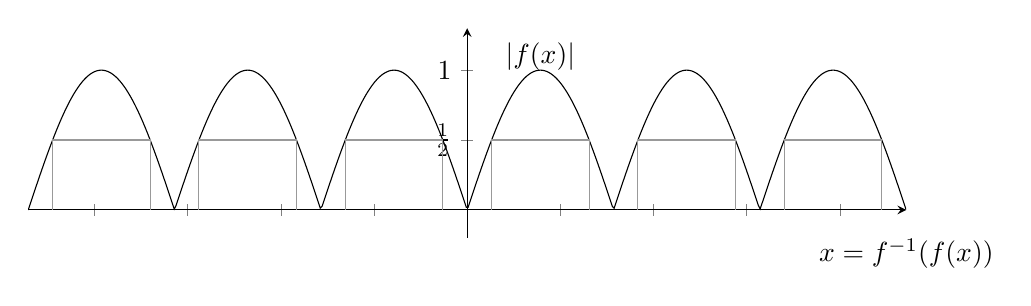
\begin{tikzpicture}
\begin{axis}[
height=0.35\textwidth,
width=1.05\textwidth,
axis lines = middle,
x label style={at={(current axis.right of origin)},anchor=north, below=2.5mm},
xlabel = {$x = f^{-1}(f(x))$},
xmin=-3*pi, xmax=3*pi,
ymin=-0.2, ymax=1.3,
ytick={1/2,1},
yticklabels={$\frac{1}{2}$,$1$},
xticklabels=\empty,
]
\node at (pi/2,1.1) {$|f(x)|$};
\addplot[domain=-3*pi:3*pi,samples=500] {abs(sin(deg(x)))};
\addplot[gray!80] coordinates {(pi/6,0) (pi/6,1/2) (5*pi/6,1/2) (5*pi/6,0)};
\addplot[gray!80] coordinates {(7*pi/6,0) (7*pi/6,1/2) (11*pi/6,1/2) (11*pi/6,0)};
\addplot[gray!80] coordinates {(13*pi/6,0) (13*pi/6,1/2) (17*pi/6,1/2) (17*pi/6,0)};
\addplot[gray!80] coordinates {(-1*pi/6,0) (-1*pi/6,1/2) (-5*pi/6,1/2) (-5*pi/6,0)};
\addplot[gray!80] coordinates {(-7*pi/6,0) (-7*pi/6,1/2) (-11*pi/6,1/2) (-11*pi/6,0)};
\addplot[gray!80] coordinates {(-13*pi/6,0) (-13*pi/6,1/2) (-17*pi/6,1/2) (-17*pi/6,0)};
\end{axis}
\end{tikzpicture}\\
\textbf{Figure 8: Lower bound of $|\sin(x)|$ in each sub-interval $(k\pi, (k+1)\pi]$.}
\end{center}
Therefore, we get that,
\begin{eqnarray}
\nonumber
\lim_{n\to\infty}\sum_{k=-n}^{n-1}\int_{k\pi}^{(k+1)\pi}|\sin(x)| dm \geq \lim_{n \to \infty} 2n \times \frac{\pi}{3} = \infty,
\end{eqnarray}
so $f(x)=\sin(x)$ is not Lebesgue integrable.\\\\
\textbf{Remark:} A Borel function $f:\Omega \to \mathbb{R}$ is Riemann integrable, if and only if the set of points of discontinuity has Lebesgue measure $0$. In general, if $f$ is Riemann integrable, then it is Lebesgue integrable.\\\\
A useful result arises from the following exercise, which is related to an important notion that we investigate later on.
\begin{center}
	\noindent\rule{12cm}{0.4pt}
\end{center}
\textbf{Exercise 4.3.1.} Let $(\Omega, \mathcal{F}, \mu)$ be a measure space and $f:\Omega \to \mathbb{R}$ a Borel function. Show that, if $\mu(A) = 0$ for some $A\in\mathcal{F}$, then $\int_\Omega f\mathds{1}_A d\mu = 0$.\\\\
\textit{Solution.} We can write $f = f^+ - f^-$, and consider an increasing sequence of non-negative simple functions $(f_i^+)_{i\geq1}$ such that, $f^+ = \lim_{i\to\infty}f_i^+$. In particular, $f_k^+ = \sum_{j=1}^{n_k}a_j\mathds{1}_{A_j}$, where $a_i \geq 0$ and $A_i \in \mathcal{F}$, $i \geq 1$, with $A_i \cap A_j = \emptyset$, $i \neq j$. Then, if $\mu(A) = 0$ for some $A\in\mathcal{F}$, it follows that,
\begin{eqnarray}
\nonumber
\int_\Omega f^+ \mathds{1}_A d\mu &=& \lim_{i\to\infty} \int_\Omega f_i^+ \mathds{1}_A d\mu \ \ \ \ \ \text{(by Theorem 4.2.1)} \\
\nonumber
&=& \lim_{i\to\infty} \sum_{j=1}^{n_i} a_j \int_\Omega \mathds{1}_{A_j} \mathds{1}_A d\mu \\
\nonumber
&=& \lim_{i\to\infty} \sum_{j=1}^{n_i} a_j \mu(A \cap A_j) \ \ \ \ \ \text{(integral of indicator function)} \\
\nonumber
&=& \lim_{i\to\infty} \sum_{j=1}^{n_i} a_j \times 0 = 0.
\end{eqnarray}
By symmetry, we can argue in the same way for $f^-$, so that indeed,
\begin{eqnarray}
\nonumber
\int_\Omega f\mathds{1}_A d\mu = 0.
\end{eqnarray}
It is worth noting that, this result applies to any Borel function. In other words, given an $\mathcal{F}$-measurable set $A$ with $\mu$ measure $0$, then the integral of $f$ over $A$ with respect to $\mu$ has to be $0$.
\begin{center}
	\noindent\rule{12cm}{0.4pt}
\end{center}
\textbf{Example 4.3.2.} Let $\Omega = [0,1]$ be a sample space. At the beginning of section 4.1, we motivate the idea of Lebesgue integral through the indicator function $f(\omega) = \mathds{1}_{\mathbb{Q}}(\omega), \ \forall \omega \in [0,1]$, but here we show this formally. Let $\tilde{f} = 0$, so $f(\omega) = \tilde{f}(\omega), \ \forall \omega \in [0,1] \setminus \mathbb{Q}$. From Exercise 4.3.1, since $m(\mathbb{Q} \cap [0,1]) = 0$, then $\int_{\mathbb{Q} \cap [0,1]} f dm = 0$. Thus, we get that,
\begin{eqnarray}
\nonumber
\int_{[0,1]} f dm &=& \int_{\mathbb{Q}\cap[0,1]}f dm + \int_{[0,1]\setminus\mathbb{Q}}f dm\\
\nonumber
&=&  0 + \int_{[0,1]\setminus\mathbb{Q}}\tilde{f} dm = 0.
\end{eqnarray}
\subsection{The Radon-Nikodym Theorem}
Intuitively, given a measure space and a non-negative Borel function, property (c) from Proposition 4.3.1 tells us that, we can construct another measure via the integral.\\\\
\textbf{Example 4.4.1.} Let $(\mathbb{R},\mathcal{B}(\mathbb{R}),m)$ be a measure space, and consider the non-negative Borel function $g(x) = \lambda e^{-\lambda x}\mathds{1}_{[0,\infty)}(x), \ \forall x \in \mathbb{R}$, where $\lambda > 0$. Then,
\begin{eqnarray}
\nonumber
\mathbb{P}_{\lambda}(B) := \int_B g dm  = \int_{\mathbb{R}} g\mathds{1}_B dm, \ \forall B \in \mathcal{B}(\mathbb{R}),
\end{eqnarray}
defines a measure on $(\mathbb{R},\mathcal{B}(\mathbb{R}))$, by Proposition 4.3.1 (c). In fact, $\mathbb{P}_{\lambda}$ is a probability measure, since
\begin{eqnarray}
\nonumber
\mathbb{P}_{\lambda}(\mathbb{R}) = \int_{\mathbb{R}}  \lambda e^{-\lambda x}\mathds{1}_{[0,\infty)}dm = \int_0^{\infty} \lambda e^{-\lambda x} dm = 1,
\end{eqnarray}
and is known as the Exponential distribution with parameter $\lambda$, where $g$ is called the density of the distribution.\\\\
\noindent\fbox{%
	\parbox{\textwidth}{%
		\textbf{Definition 4.4.1. Absolute Continuity between measures $\nu$ and $\mu$} \\ Let $\nu,\mu:\mathcal{F}\to[0,\infty)$ be measures on a given measurable space $(\Omega,\mathcal{F})$. We say that $\nu$ is absolutely continuous with respect to $\mu$, if
		\begin{center}
			$\forall A \in \mathcal{F}$ with $\mu(A) = 0 \implies \nu(A) = 0$,
		\end{center}
	and we write $\nu \ll \mu$.
	}%
}\\\\\\
\noindent\fbox{%
	\parbox{\textwidth}{%
		\textbf{Definition 4.4.2. The Radon-Nikodym derivative $f$} \\ Let $(\Omega,\mathcal{F},\mu)$ be a measure space and $f:\Omega\to\mathbb{R}$ a Borel function. If $\nu:\mathcal{F}\to[0,\infty)$ is a measure on $(\Omega,\mathcal{F})$ defined by,
		\begin{center}
			$\nu(A) := \int_A f d\mu, \ \forall A \in \mathcal{F}$,
		\end{center}
		we say that $f$ is the Radon-Nikodym derivative, or density, of $\nu$ with respect to $\mu$, and we write $f = \frac{d\nu}{d\mu}$.
	}%
}\\\\\\
At this point, it is substantial to take into consideration that $\nu$ as in Definition 4.4.2 defines a measure on a given measurable space $(\Omega,\mathcal{F})$, by Proposition 4.3.1 (c), so that the Radon-Nikodym derivative $f$ is well-defined. Thereby, we go through some examples that conceptualize the underlying meaning of absolutely continuous measures.\\\\
\textbf{Example 4.4.2.} Let $(\mathbb{N},\mathcal{P}(\mathbb{N}))$ be a measurable space. Consider the Dirac measure at a point $k \in \mathbb{N}$ given by,
\begin{center}
	$\delta_k(A) =
	\begin{cases}
	1, & k \in A\\
	0, & k \notin A
	\end{cases}$
\end{center}
and the counting measure $\mu_C(A) = \sum_{i=1}^{\infty}\delta_i(A)$. Clearly, if a $\mathcal{P}(\mathbb{N})$-measurable set $A$ has $\mu_C$ measure $0$, then it has to have $\delta_k$ measure $0$, by construction. Hence, $\delta_k$ is absolutely continuous with respect to $\mu_C$, i.e. $\delta_k \ll \mu_C$. \\\\
\textbf{Remark:} Even though an indicator function and a Dirac measure seem to coincide, this is not the case at all and it is important to be able to distinguish between them. Given a measurable space $(\Omega,\mathcal{F})$ and $A \in \mathcal{F}$, an indicator function on $A$ is a Borel function $\mathds{1}_A:\Omega\to\{0,1\}$, whereas a Dirac measure on $k \in \Omega$ is a map $\delta_k:\mathcal{F}\to\{0,1\}$. In other words, $\mathds{1}_A$ checks whether a point lies in $A$, whereas $\delta_k$ checks whether an $\mathcal{F}$-measurable set $A$ contains $k$.\\\\
\textbf{Example 4.4.3.} Let $(\mathbb{R},\mathcal{B}(\mathbb{R}),m)$ be a measure space and $\mu_C$ a counting measure on $\mathbb{R}$, which leads to the following cases:
\begin{enumerate}[(a)]
	\item $\mu_C(A) = \infty \implies A$ is at least countable Borel set.
	\item $\mu_C(A) = N < \infty \implies A = \{a_1,...,a_N\}$, for some $a_1,...,a_N \in \mathbb{R}$,
	\item $\mu_C(A) = 0 \implies A = \emptyset$.
\end{enumerate}
In the case of (c), we can see that it has to be that, $m(\emptyset)=0$, so that $m$ is absolutely continuous with respect to $\mu_C$, i.e. $m \ll \mu_C$. The converse is not true, since $m(\mathbb{N}) = 0$, but $\mu_C(\mathbb{N}) = \infty$ from case (a).\\\\
\textbf{Example 4.4.4.} Let $(\Omega,\mathcal{F},\mu)$ be a measure space and $\nu(A) = \int_A f d\mu, \ A\in\mathcal{F}$, be a measure on $(\Omega,\mathcal{F})$, where $f$ is the Radon-Nikodym derivative of $\nu$ with respect to $\mu$. Then, we know from Exercise 4.3.1 that, if $\mu(A) = 0$, then
\begin{center}
	$\nu(A) = \int_A f d\mu = 0$,
\end{center}
so that $\nu$ is absolutely continuous with respect to $\mu$, i.e. $\nu\ll\mu$. We question whether the converse implication holds, i.e. if $\nu$ is absolutely continuous with respect to $\mu$, then there is a Borel function $f:\Omega\to\mathbb{R}$ such that, $\nu(A) = \int_A f d\mu, \ \forall A \in \mathcal{F}$. This is precisely the Radon-Nikodym theorem, which is stated onwards.\\\\
Analogously to continuity notions in Real Analysis, the definition of absolutely continuous measures can be expressed in the usual $\epsilon-\delta$ form.\\\\
\noindent\fbox{%
	\parbox{\textwidth}{%
		\textbf{Proposition 4.4.1. Alternative definition of Absolutely Continuous measures $\nu$ and $\mu$} \\ Let $\nu,\mu:\mathcal{F}\to[0,\infty)$ be measures on a given measurable space $(\Omega,\mathcal{F})$. Then, $\nu$ is absolutely continuous with respect to $\mu$, if and only if, $\forall \epsilon>0, \ \exists \delta > 0$ such that,
		\begin{center}
			$\forall A \in \mathcal{F}$ with $\mu(A) < \delta \implies \nu(A) < \epsilon$.
		\end{center}
	}%
}\\\\\\
\textbf{Remarks:}
\begin{enumerate}[1.]
	\item In general, $\nu\ll\mu$ does not imply $\mu\ll\nu$.
	\item If we have both $\nu\ll\mu$ and $\mu\ll\nu$, then we say that $\nu$ and $\mu$ are equivalent, and we write $\nu \sim \mu$. In this case, $\nu(A) = 0$, if and only if $\mu(A) = 0$, so $\nu$ and $\mu$ agree on the sets with measure $0$. In fact, ‘$\sim$’ is an equivalence relation, since it is reflexive, symmetric and transitive.
\end{enumerate}
\textbf{Example 4.4.2. (continued)} Let $\nu_1(A) := \int_A \sum_{k=0}^{n}\binom{n}{k}p^k(1-p)^{n-k}\mathds{1}_{\{k\}} d\mu_C, \ p\in(0,1), \ n \in \mathbb{N}$, where $\frac{d\nu_1}{d\mu_C} = \sum_{k=0}^{n}\binom{n}{k}p^k(1-p)^{n-k}\mathds{1}_{\{k\}}$ is the Radon-Nikodym derivative of $\nu_1$ with respect to $\mu_C$. Then, we can simplify $\nu_1$ by,
\begin{eqnarray}
\nonumber
\nu_1(A) &=& \int_A \sum_{k=0}^{n}\binom{n}{k}p^k(1-p)^{n-k}\mathds{1}_{\{k\}} d\mu_C \\
\nonumber
&=& \sum_{k=0}^{n}\binom{n}{k}p^k(1-p)^{n-k}\int_A \mathds{1}_{\{k\}} d\mu_C\\
\nonumber
&=& \sum_{k=0}^{n}\binom{n}{k}p^k(1-p)^{n-k}\mu_C(A \cap k)\\
\nonumber
&=& \sum_{k=0}^{n}\binom{n}{k}p^k(1-p)^{n-k}\delta_k(A)\\
\nonumber
&=& \sum_{k \in A}\binom{n}{k}p^k(1-p)^{n-k}, \ \forall A \subseteq \{0,1,...,n\} \in \mathcal{P}(\mathbb{N}),
\end{eqnarray}
and is known as the Binomial distribution with parameters $n$ and $p$, where $\frac{d\nu_1}{d\mu_C}$ is the density of the distribution. Thus, we have $\nu_1\ll\mu_C$, but $\mu_C\ll\nu_1$ also holds. For any $A\subseteq \{0,1,...,n\}\in\mathcal{P}(\mathbb{N})$ with $\nu_1(A) = 0$,  it has to be that $A = \emptyset$, which implies that $\mu_C(A) = 0$. Now, set $\nu_2(A) := \int_A \sum_{k=0}^{\infty}\frac{e^{-\lambda}\lambda^k}{k!}\mathds{1}_{\{k\}} d\mu_C, \ \lambda > 0$, where $\frac{d\nu_2}{d\mu_C} = \sum_{k=0}^{\infty}\frac{e^{-\lambda}\lambda^k}{k!}\mathds{1}_{\{k\}}$ is the Radon-Nikodym derivative of $\nu_2$ with respect to $\mu_C$. Similarly, $\nu_2$ can be simplified as,
\begin{eqnarray}
\nonumber
\nu_2(A) = \sum_{k \in A}\frac{e^{-\lambda}\lambda^k}{k!}, \ \forall A \in \mathcal{P}(\mathbb{N}),
\end{eqnarray}
and is known as the Poisson distribution with parameter $\lambda$, where $\frac{d\nu_2}{d\mu_C}$ is the density of the distribution. Thus, we have $\nu_2\ll\mu_C$. We can argue as in the case of $\nu_1$ that $\mu_C\ll\nu_2$. Observe that, when restricted to sets $A \subseteq \{0,1,...,n\}$, $\nu_1 \sim \mu_C$ and $\nu_2 \sim \mu_C$, so by transitivity, it follows that $\nu_1 \sim \nu_2$. Both $\nu_1$ and $\nu_2$ are discrete probability distributions that assign positive probability at each point in $A \subseteq \{0,1,...,n\}$, unless it is the empty set. In general, equivalent measures act as different frames over the given measurable space, while preserving measure $0$ on given measurable sets. Note that, equivalence does not hold at any point in $\mathbb{N}$, since $\nu_2$ assigns positive probability for any point in $\mathbb{N}$, whereas $\nu_1$ is restricted up to given $n\in\mathbb{N}$, which follows by construction of these probability distributions.\\\\
\textbf{Example 4.4.3. (continued)} Let $\nu_1(A) := \int_A \frac{1}{\sqrt{2\pi\sigma^2}}e^{-\frac{(x-\mu)^2}{2\sigma^2}} dm, \ x,\mu \in \mathbb{R}, \sigma > 0$,\\ where $\frac{d\nu_1}{dm} = \frac{1}{\sqrt{2\pi\sigma^2}}e^{-\frac{(x-\mu)^2}{2\sigma^2}}$ is the Radon-Nikodym derivative of $\nu_1$ with respect to $m$. Clearly, $\nu_1$ is known as the Normal distribution with parameters $\mu$ and $\sigma^2$, where $\frac{d\nu_1}{dm}$ is the density of the distribution. Indeed, $\nu_1$ and $m$ are equivalent. Moreover, $\nu_2(A) := \int_A \lambda e^{-\lambda x}\mathds{1}_{[0,\infty)} dm$ is known as the Exponential distribution with parameter $\lambda > 0$, where $\frac{d\nu_2}{dm} = e^{-\lambda x}\mathds{1}_{[0,\infty)}$ is the density of the distribution. However, $m$ is not absolutely continuous with respect to $\nu_2$, since for $A \subseteq (-\infty,0)$, we have $\nu_2(A) = 0$, but $m(A) \neq 0$.\\\\
We state without proof the powerful Randon-Nikodym theorem, which unravels the converse to Example 4.4.4.\\\\
\noindent\fbox{%
	\parbox{\textwidth}{%
		\textbf{Theorem 4.4.1. The Radon-Nikodym Theorem} \\ Let $\nu,\mu:\mathcal{F}\to[0,\infty)$ be $\sigma$-finite measures on a given measurable space $(\Omega,\mathcal{F})$. Then, $\nu\ll\mu$, if and only if there exists a function $f:\Omega\to\mathbb{R}$, such that
		\begin{center}
			$\nu(A) = \int_A f d\mu, \ \forall A \in \mathcal{F}$,
		\end{center}
		where $f = \frac{d\nu}{d\mu}$ is the Radon-Nikodym derivate of $\nu$ with respect to $\mu$.
	}%
}\\\\\\
To show existence of $f$ is quite involved, so we skip the proof. A useful property of the Radon-Nikodym derivative is the following.\\\\
\noindent\fbox{%
	\parbox{\textwidth}{%
		\textbf{Proposition 4.4.2. Chain rule of the Radon-Nikodym derivative $f$} \\ Let $\nu,\mu:\mathcal{F}\to[0,\infty)$ be measures on a given measurable space $(\Omega,\mathcal{F})$, such that $\nu\ll\mu$ and $g:\Omega\to\mathbb{R}$ a Borel function. Then, $g$ is $\nu$-integrable, if and only if $g\frac{d\nu}{d\mu}$ is $\mu$-integrable, and
		\begin{center}
			$\int_\Omega g d\nu = \int_\Omega g \frac{d\nu}{d\mu} d\mu$.
		\end{center}
	}%
}\\\\\\
\textit{Proof.} As usual, we show this by constructing a sequence of non-negative simple functions. We write $g = g^+ - g^-$, and consider the increasing sequence of non-negative simple functions $(g_i^+)_{i\geq1}, \ (g_i^-)_{i\geq1}$, such that $\lim_{i\to\infty}g_i^+ = g^+, \ \lim_{i\to\infty}g_i^- = g^-$. In particular, $g_k^+ = \sum_{j=1}^{n_k}a_j\mathds{1}_{A_j}$, where $a_i\geq0$ and $A_i\in\mathcal{F}$, $i\geq1$, with $A_i \cap A_j = \emptyset$, $i \neq j$. By the Monotone-Convergence theorem, we have that,
\begin{eqnarray}
\nonumber
\int_\Omega g^+ d\nu = \lim_{i\to\infty} \int_\Omega g_i^+ d\nu = \lim_{i\to\infty} \sum_{j=1}^{n_i}a_j \int_\Omega \mathds{1}_{A_j} d\nu.
\end{eqnarray}
Now, observe that,
\begin{eqnarray}
\nonumber
\int_\Omega \mathds{1}_{A_j} d\nu = \nu(A_j) = \int_{A_j} \frac{d\nu}{d\mu} d\mu,
\end{eqnarray}
so it follows that,
\begin{eqnarray}
\nonumber
\int_\Omega g^+ d\nu &=& \lim_{i\to\infty}\sum_{j=1}^{n_i}a_j \int_{A_j} \frac{d\nu}{d\mu} d\mu\\
\nonumber
&=& \int_\Omega \lim_{i\to\infty}\sum_{j=1}^{n_i}a_j \mathds{1}_{A_j} \frac{d\nu}{d\mu} d\mu\\
\nonumber
&=& \int_\Omega g^+ \frac{d\nu}{d\mu} d\mu.
\end{eqnarray}
We can argue in the same way for $g^-$, so that indeed,
\begin{eqnarray}
\nonumber
\int_\Omega g d\nu = \int_\Omega g \frac{d\nu}{d\mu} d\mu.
\end{eqnarray}
${}$ \hfill $\square$ \\\\
\textbf{Remark:} In the case where we have probability measures $\mathbb{P},\mathbb{Q}$ on a measurable space $(\Omega,\mathcal{F})$, such that $\mathbb{Q}\ll\mathbb{P}$, and $X:\Omega\to\mathbb{R}$ a real-valued random variable which is $\mathbb{Q}$-integrable, then
\begin{center}
	$\mathbb{E}^{\mathbb{Q}}[X] = \mathbb{E}^{\mathbb{P}}\left[X\frac{d\mathbb{Q}}{d\mathbb{P}}\right]$.
\end{center}
\textbf{Example 4.4.5.} Let $(\Omega,\mathcal{F},\mathbb{P})$ be a probability space and $X \sim N(0,1)$, i.e. $X$ is a standard Normal random variable with probability distribution,
\begin{center}
	$\mathbb{P}[X \in A] = \int_A \frac{1}{\sqrt{2\pi}} e^{-\frac{x^2}{2}} dm, \ \forall A \in \mathcal{B}({\mathbb{R}})$.
\end{center}
Note that, $X + \theta \sim N(\theta,1), \ \theta\in\mathbb{R}$, under $\mathbb{P}$. We define another measure $\mathbb{Q}$, such that\\ $X + \theta \sim N(0,1)$, under $\mathbb{Q}$. Take $\frac{d\mathbb{Q}}{d\mathbb{P}} = e^{-\theta X - \frac{\theta^2}{2}}$ and by Proposition 4.4.2, we get that,
\begin{eqnarray}
\nonumber
\mathbb{E}^{\mathbb{Q}}[e^{t(X+\theta)}] &=& \mathbb{E}^{\mathbb{P}}[e^{t(X+\theta)}e^{-\theta X - \frac{\theta^2}{2}}]\\
\nonumber
&=& e^{\theta t - \frac{\theta^2}{2}} \mathbb{E}^{\mathbb{P}}[e^{(t-\theta)X}]\\
\nonumber
&=& e^{\theta t - \frac{\theta^2}{2}} e^{\frac{(t-\theta)^2}{2}} = e^{\frac{t^2}{2}}, \ t \in \mathbb{R},
\end{eqnarray}
so by uniqueness of moment generating functions, $X + \theta \sim N(0,1)$, under $\mathbb{Q}$. This tells us that $\mathbb{Q}$ denotes a standard normal distribution shifted by $-\theta$, so as to normalise $X + \theta$.
\subsection{Convergence Theorems}
So far, we know about the Monotone-Convergence theorem, which in fact encapsulates one of the examinable convergence notions. At this point, we require an associated concept to convergence.\\\\
\noindent\fbox{%
	\parbox{\textwidth}{%
		\textbf{Definition 4.5.1. $\mu$-Null $\mathcal{F}$-measurable set and Almost everywhere} \\ Let $(\Omega,\mathcal{F},\mu)$ be a measure space and $A\in\mathcal{F}$. Then, $A$ is called a $\mu$-null set, if $\mu(A) = 0$. We say that $A$ holds $\mu$-almost everywhere, if $\mu(A^c) = 0$, abbreviated by ‘$\mu$-a.e.’
	}%
}\\\\\\
\textbf{Remark:} In the case of $(\Omega,\mathcal{F},\mathbb{P})$ being a probability space, we say that $A\in\mathcal{F}$ holds $\mathbb{P}$-almost surely, if $\mathbb{P}(A^c) = 0$, abbreviated by ‘$\mathbb{P}$-a.s.’ \\\\
It is often the case that a property suffices to hold almost everywhere, as the complement of that  is redundant by the measure.\\\\
\noindent\fbox{%
	\parbox{\textwidth}{%
		\textbf{Lemma 4.5.1. $\mu$-a.e. Borel functions $f$ and $g$} \\ Let $(\Omega,\mathcal{F},\mu)$ be a measure space and $f,g:\Omega\to\mathbb{R}$ Borel functions. If $f$ is $\mu$-integrable and $f = g$ $\mu$-a.e., then
		\begin{center}
			$\int_\Omega f d\mu = \int_\Omega g d\mu$.
		\end{center}
	}%
}\\\\\\
\textit{Proof.} Set $E := \{f=g\} \in \mathcal{F}$, so that $E^c = \{f \neq g\}$, where $\mu(E^c) = 0$. Therefore, by Exercise 4.3.1, it follows that,
\begin{eqnarray}
\nonumber
\int_{E^c} f d\mu = 0 = \int_{E^c} g d\mu,
\end{eqnarray}
so that indeed,
\begin{eqnarray}
\nonumber
\int_\Omega f d\mu = \int_E f d\mu = \int_E g d\mu = \int_\Omega g d\mu.
\end{eqnarray}
${}$ \hfill $\square$\\\\
\noindent\fbox{%
	\parbox{\textwidth}{%
		\textbf{Definition 4.5.2. Convergence $\mu$-a.e.} \\ Let $(\Omega,\mathcal{F},\mu)$ be a measure space and $(f_n)_{n\geq1}, f$ be Borel functions. We say that, $(f_n)_{n\geq1}$ converges to $f$ $\mu$-a.e., if and only if
		\begin{center}
			$\mu(\{\lim_{n\to\infty}f_n = f\}^c) = 0$.
		\end{center}
		Then, we write $f_n \xrightarrow{\mu\text{-a.e.}} f$.
	}%
}\\\\\\
\noindent\fbox{%
	\parbox{\textwidth}{%
		\textbf{Definition 4.5.3. Convergence in measure} \\ Let $(\Omega,\mathcal{F},\mu)$ be a measure space and $(f_n)_{n\geq1}, f$ be Borel functions. We say that, $(f_n)_{n\geq1}$ converges to $f$ in measure, if and only if $\forall \epsilon>0$,
		\begin{center}
			$\lim_{n\to\infty}\mu(|f_n - f| > \epsilon) = 0$.
		\end{center}
		Then, we write $f_n \xrightarrow{\mu} f$.
	}%
}\\\\\\
\noindent\fbox{%
	\parbox{\textwidth}{%
		\textbf{Definition 4.5.4. Convergence in $\mathcal{L}^p$} \\ Let $(\Omega,\mathcal{F},\mu)$ be a measure space and $(f_n)_{n\geq1}, f$ be Borel functions with $f \in \mathcal{L}^p(\mu), \ p\in[1,\infty)$, i.e.
		\begin{center}
			$\int_\Omega |f|^p d\mu < \infty$.
		\end{center}
		We say that, $(f_n)_{n\geq1}$ converges to $f$ in $\mathcal{L}^p$, if and only if
		\begin{center}
			$\lim_{n\to\infty}\int_\Omega |f_n - f|^p d\mu = 0$.
		\end{center}
		Then, we write $f_n \xrightarrow{\mathcal{L}^p} f$.
	}%
}\\\\\\
Naturally, we ask how these modes of convergence interrelate with one another. First, let us introduce Chebyshev's inequality, which acts as a sharp bound for functions in $\mathcal{L}^p(\mu)$.\\\\
\noindent\fbox{%
	\parbox{\textwidth}{%
		\textbf{Lemma 4.5.2. Chebyshev's inequality} \\ Let $(\Omega,\mathcal{F},\mu)$ be a measure space and $f:\Omega\to\mathbb{R}$ a Borel function. Then, $\forall \epsilon \geq 0$ and $\alpha \geq 0$, 
		\begin{center}
			$\mu(\{|f|\geq\epsilon\}) \leq \frac{1}{\epsilon^\alpha}\int_{\Omega} |f|^\alpha d\mu$.
		\end{center}
	}%
}\\\\\\
\textit{Proof.} $\forall \epsilon \geq 0$ and $\alpha \geq 0$, we have that,
\begin{eqnarray}
\nonumber
\int_\Omega |f|^\alpha d\mu \geq \int_{\{|f| \geq \epsilon\}} |f|^\alpha d\mu \geq \int_{\{|f| \geq \epsilon\}} \epsilon^\alpha d\mu = \epsilon^\alpha \int_\Omega \mathds{1}_{\{|f| \geq \epsilon\}} = \epsilon^\alpha \mu(\{|f|\geq\epsilon\}),
\end{eqnarray}
and by rearranging, the result follows.\\
${}$ \hfill $\square$\\\\
\textbf{Remark:} In the setting of $(\Omega,\mathcal{F},\mathbb{P})$ being a probability space and $X:\Omega\to\mathbb{R}$ a real-valued random variable, $\forall \epsilon \geq 0$ and $\alpha \geq 0$,
\begin{center}
	$\mathbb{P}(|X| \geq \epsilon) \leq \frac{1}{\epsilon^\alpha}\mathbb{E}[|X|^\alpha]$,
\end{center}
which is sometimes referred to as Markov's inequality. We can, in turn, bound deviation from the mean using the variance of $X$ by,
\begin{center}
	$\mathbb{P}(|X - \mathbb{E}[X]| \geq \epsilon) \leq \frac{1}{\epsilon^2}Var[X]$.
\end{center}
\begin{center}
	\noindent\rule{12cm}{0.4pt}
\end{center}
\textbf{Exercise 4.5.1.} Let $(\Omega,\mathcal{F},\mu)$ be a measure space and $f \geq 0$ a Borel function. Show that, $\int_\Omega f d\mu = 0$, if and only if $f = 0$ $\mu$-a.e. \\\\
\textit{Solution.} The first direction follows immediately. Now, suppose that $\int_\Omega f d\mu = 0$. It suffices to show that, $\mu(\{f > 0\}) = 0$, since we can then conclude that $f = 0$ $\mu$-a.e. Let $A_n := \{f\geq\frac{1}{n}\} \in \mathcal{F}$, so that $A_k \subseteq A_{k+1}, \ \forall k \in \mathbb{N}$, and set $A := \{f>0\}$. Hence, by Chebyshev's inequality and continuity from below, we get that,
\begin{eqnarray}
\nonumber
\mu(A_n) \leq n\int_\Omega f d\mu = 0, \ \forall n\in\mathbb{N} \implies  \mu(A) = \mu(\{f>0\}) = \lim_{n\to\infty}\mu(A_n) = 0.
\end{eqnarray}
\begin{center}
	\noindent\rule{12cm}{0.4pt}
\end{center}
By applying Chebyshev's inequality, we can deduce that convergence in $\mathcal{L}^p$ implies convergence in measure.\\\\
\noindent\fbox{%
	\parbox{\textwidth}{%
		\textbf{Lemma 4.5.3. Convergence in $\mathcal{L}^p$ implies convergence in measure} \\ Let $(\Omega,\mathcal{F},\mu)$ be a measure space and $(f_n)_{n\geq1}, f$ be Borel functions. Then,
		\begin{center}
			$f_n \xrightarrow{\mathcal{L}^p} f \implies f_n \xrightarrow{\mu} f$.
		\end{center}
	}%
}\\\\\\
\textit{Proof.} Since $f_n \xrightarrow{\mathcal{L}^p} f$, for some $p \geq 1$, then
\begin{eqnarray}
\nonumber
\lim_{n\to\infty}\int_\Omega |f_n - f|^p d\mu = 0.
\end{eqnarray}
By Chebyshev's inequality, $\forall \epsilon \geq 0$, it follows that,
\begin{eqnarray}
\nonumber
\mu(|f_n - f| > \epsilon) \leq \frac{1}{\epsilon^p}\int_\Omega |f_n-f|^p d\mu \xrightarrow{n\to\infty} 0,
\end{eqnarray}
thus $f_n$ converges to $f$ in measure, i.e. $f_n \xrightarrow{\mu} f$.\\
${}$ \hfill $\square$ \\\\
However, in general, convergence almost everywhere does not imply convergence in $\mathcal{L}^p$ or in measure.\\\\
\textbf{Example 4.5.1.} Let $(\mathbb{R},\mathcal{B}(\mathbb{R}),m)$ be a measure space, and consider the sequence of Borel functions $\{f_n\}_{n\geq1}$, where $f_n = \mathds{1}_{[n,n+1)}$, which is known as the ‘traveling wave’. Notice that,
\begin{eqnarray}
\nonumber
m\left(\left\{\lim_{n\to\infty}f_n = 0\right\}^c\right) = m(\{f_n \nrightarrow 0\}) = 0,
\end{eqnarray}
so that, $f_n \xrightarrow{m\text{-a.e.}} 0$. However, we have that,
\begin{eqnarray}
\nonumber
\int_\Omega |f_n|^p dm = 1, \ \forall p \geq 1,
\end{eqnarray}
which implies that $f_n$ does not converge to $0$ in $\mathcal{L}^p$.\\\\
\textbf{Example 4.5.2.} Let $(\mathbb{R},\mathcal{B}(\mathbb{R}),m)$ be a measure space, and consider the sequence of Borel functions $(f_{n,k})_{n\geq0}$, where $f_{n,k} = \mathds{1}_{[\frac{k}{2^n},\frac{k+1}{2^n})}, \ k = 0,...,2^n-1$, which is known as the ‘dancing wave’. Figure 9 below illustrates the construction of $f_{n,k}$.
\begin{center}
\begin{tikzpicture}
\begin{axis}[
width=0.3\textwidth,
axis lines = middle,
xmin=0,xmax=1,
ymin=0,ymax=1.2,
ytick = {0,1},
yticklabels={$0$,$1$},
xtick = {0,1},
xticklabels={$0$,$1 \atop {}$},
]
\node at (0.5,0.85) {$f_{0,0}$};
\addplot[domain=0:1,samples=100] {1};
\addplot[color=black,fill=white,only marks,mark=*] coordinates {(0,1)};
\addplot[color=black,only marks,mark=*] coordinates {(1,1)};
\end{axis}
\end{tikzpicture}
\begin{tikzpicture}
\begin{axis}[
width=0.3\textwidth,
axis lines = middle,
xmin=0,xmax=1,
ymin=0,ymax=1.2,
ytick = {0,1},
yticklabels={$0$,$1$},
xtick = {0,1/2},
xticklabels={$0$,$\frac{1}{2}$},
]
\node at (0.25,0.85) {$f_{1,0}$};
\addplot[domain=0:1/2,samples=100] {1};
\addplot[color=black,fill=white,only marks,mark=*] coordinates {(0,1)};
\addplot[color=black,only marks,mark=*] coordinates {(1/2,1)};
\end{axis}
\end{tikzpicture}
\begin{tikzpicture}
\begin{axis}[
width=0.3\textwidth,
axis lines = middle,
xmin=0,xmax=1,
ymin=0,ymax=1.2,
ytick = {0,1},
yticklabels={$0$,$1$},
xtick = {1/2,1},
xticklabels={$\frac{1}{2}$,$1 \atop {}$},
]
\node at (0.75,0.85) {$f_{1,1}$};
\addplot[domain=1/2:1,samples=100] {1};
\addplot[color=black,fill=white,only marks,mark=*] coordinates {(1/2,1)};
\addplot[color=black,only marks,mark=*] coordinates {(1,1)};
\end{axis}
\end{tikzpicture}\\
\begin{tikzpicture}
\begin{axis}[
width=0.3\textwidth,
axis lines = middle,
xmin=0,xmax=1,
ymin=0,ymax=1.2,
ytick = {0,1},
yticklabels={$0$,$1$},
xtick = {0,1/4},
xticklabels={$0$,$\frac{1}{4}$},
]
\node at (0.125,0.85) {$f_{2,0}$};
\addplot[domain=0:1/4,samples=100] {1};
\addplot[color=black,fill=white,only marks,mark=*] coordinates {(0,1)};
\addplot[color=black,only marks,mark=*] coordinates {(1/4,1)};
\end{axis}
\end{tikzpicture}
\begin{tikzpicture}
\begin{axis}[
width=0.3\textwidth,
axis lines = middle,
xmin=0,xmax=1,
ymin=0,ymax=1.2,
ytick = {0,1},
yticklabels={$0$,$1$},
xtick = {1/4,1/2},
xticklabels={$\frac{1}{4}$,$\frac{1}{2}$},
]
\node at (0.375,0.85) {$f_{2,1}$};
\addplot[domain=1/4:1/2,samples=100] {1};
\addplot[color=black,fill=white,only marks,mark=*] coordinates {(1/4,1)};
\addplot[color=black,only marks,mark=*] coordinates {(1/2,1)};
\end{axis}
\end{tikzpicture}
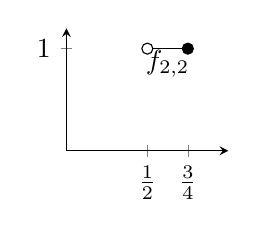
\begin{tikzpicture}
\begin{axis}[
width=0.3\textwidth,
axis lines = middle,
xmin=0,xmax=1,
ymin=0,ymax=1.2,
ytick = {0,1},
yticklabels={$0$,$1$},
xtick = {1/2,3/4},
xticklabels={$\frac{1}{2}$,$\frac{3}{4}$},
]
\node at (0.625,0.85) {$f_{2,2}$};
\addplot[domain=1/2:3/4,samples=100] {1};
\addplot[color=black,fill=white,only marks,mark=*] coordinates {(1/2,1)};
\addplot[color=black,only marks,mark=*] coordinates {(3/4,1)};
\end{axis}
\end{tikzpicture}
\begin{tikzpicture}
\begin{axis}[
width=0.3\textwidth,
axis lines = middle,
xmin=0,xmax=1,
ymin=0,ymax=1.2,
ytick = {0,1},
yticklabels={$0$,$1$},
xtick = {3/4,1},
xticklabels={$\frac{3}{4}$,$1 \atop {}$},
]
\node at (0.875,0.85) {$f_{2,3}$};
\addplot[domain=3/4:1,samples=100] {1};
\addplot[color=black,fill=white,only marks,mark=*] coordinates {(3/4,1)};
\addplot[color=black,only marks,mark=*] coordinates {(1,1)};
\end{axis}
\end{tikzpicture}\\
\textbf{Figure 9: First elements of the ‘dancing wave’.}
\end{center}
In particular, as $n$ gets larger, each sub-interval gets shorter exponentially, while given $n\geq0$, $k$ ensures that, $f_{n,k}$ still oscillates between $0$ and $1$. Then, for any $p\geq1$, we have that,
\begin{eqnarray}
\nonumber
\int_\Omega |f_{n,k}|^p dm \xrightarrow{n\to\infty} 0,
\end{eqnarray}
so that $f_{n,k} \xrightarrow{\mathcal{L}^p} 0$. But, by construction of $(f_{n,k})_{n\geq0}$, we can see that,
\begin{eqnarray}
\nonumber
m\left(\left\{\lim_{n\to\infty}f_{n,k} = 0\right\}^c\right) = m(\{f_{n,k} \nrightarrow 0\}) = m([0,1)) = 1 \neq 0,
\end{eqnarray}
since for each $n\geq0$, $f_{n,k}$ covers $[0,1)$, which implies that $f_{n,k}$ does not converge to $0$ $m$-almost everywhere. \\\\
Under certain conditions, convergence almost everywhere does imply convergence in $\mathcal{L}^1$. For this matter, Fatou's Lemmas establish essential integral inequalities to be used onwards.\\\\
\noindent\fbox{%
	\parbox{\textwidth}{%
		\textbf{Lemma 4.5.4. Fatou's Lemma} \\ Let $(\Omega,\mathcal{F},\mu)$ be a measure space and $(f_n)_{n\geq1}$ a sequence of non-negative Borel functions. Then,
		\begin{center}
			$\int_\Omega\liminf_{n\to\infty}f_n d\mu \leq \liminf_{n\to\infty}\int_\Omega f_n d\mu$.
		\end{center}
	}%
}\\\\\\
\textit{Proof.} Set $g_n := \inf_{i \geq n}f_i, \ n \geq 1$, which is an increasing sequence of non-negative Borel functions, and $\lim_{n\to\infty}g_n = \liminf_{n\to\infty}f_n$. Since $g_n \leq f_i, \ \forall i \geq n$, by monotonicity of the integral, it follows that,
\begin{eqnarray}
\nonumber
\int_\Omega g_n d\mu \leq \int_\Omega f_i d\mu \implies \int_\Omega g_n d\mu \leq \inf_{i \geq n}\int_\Omega f_i d\mu,
\end{eqnarray}
where we take the infimum over all $i \geq n$ on the right hand side. By the Monotone-Convergence theorem, get that,
\begin{eqnarray}
\nonumber
\int_\Omega \lim_{n\to\infty}g_n d\mu = \int_{\Omega} \sup_{n \geq 1}g_n d\mu = \sup_{n \geq 1}\int_\Omega g_n d\mu \leq \adjustlimits{\sup}_{n \geq 1}{\inf}_{i \geq n}\int_\Omega f_i d\mu = \liminf_{n\to\infty}\int_\Omega f_n d\mu. 
\end{eqnarray}
${}$ \hfill $\square$\\\\
\noindent\fbox{%
	\parbox{\textwidth}{%
		\textbf{Lemma 4.5.5. Reverse Fatou's Lemma} \\ Let $(\Omega,\mathcal{F},\mu)$ be a measure space and $(f_n)_{n\geq1}$ a sequence of non-negative Borel functions. If there exists a non-negative Borel function $g$ that is $\mu$-integrable, such that $f_n \leq g, \ \forall n \geq 1$, then
		\begin{center}
			$\int_\Omega\limsup_{n\to\infty}f_n d\mu \geq \limsup_{n\to\infty}\int_\Omega f_n d\mu$.
		\end{center}
	}%
}\\\\\\
\textit{Proof.} This proof is quite straightforward. Set $h_n := g - f_n \geq 0, \ n \geq 1$, so that taking the limit inferior on both sides yields, $\liminf_{n\to\infty}h_n = g - \limsup_{n\to\infty}f_n$. By Lemma 4.5.4, we have that,
\begin{eqnarray}
\nonumber
\int_\Omega\liminf_{n\to\infty}h_n d\mu \leq \liminf_{n\to\infty}\int_\Omega h_n d\mu,
\end{eqnarray}
and consequently, it follows that,
\begin{eqnarray}
\nonumber
\int_\Omega\limsup_{n\to\infty}f_n d\mu \geq \limsup_{n\to\infty}\int_\Omega f_n d\mu.
\end{eqnarray}
${}$ \hfill $\square$ \\\\
\textbf{Remark:} It is not necessarily the case that we must have equality. Also, if $(f_n)_{n\geq1}$ is a sequence that contains negative Borel functions, both lemmas may fail. The following examples capture these points.\\\\
\textbf{Example 4.5.3.} Let $([0,1],\mathcal{B}([0,1]),m)$ be a measure space, where $\mathcal{B}([0,1]) = \mathcal{B}(\mathbb{R}) \cap [0,1]$. Consider the sequence of non-negative Borel functions $(f_n)_{n\geq1}$ given by,
\begin{center}
	$f_n(x) =
	\begin{cases}
	n, & x \in [0,\frac{1}{n}) \\
	0, & \text{otherwise}
	\end{cases}$
\end{center}
It is clear that, $\lim_{n\to\infty}f_n = 0$ and consequently,
\begin{eqnarray}
\nonumber
\int_{\Omega} \liminf_{n\to\infty} f_n dm = 0.
\end{eqnarray}
But, we can see that, $\int_\Omega f_n dm = 1, \ \forall n\geq1$, which implies that,
\begin{eqnarray}
\nonumber
\liminf_{n\to\infty} \int_\Omega f_n dm = 1 > 0 = \int_{\Omega} \liminf_{n\to\infty} f_n dm,
\end{eqnarray}
which is a strict inequality of Fatou's Lemma.\\\\
\textbf{Example 4.5.4.} Let $(\mathbb{R},\mathcal{B}(\mathbb{R}),m)$ be a measure space. Consider the sequence of Borel functions $(f_n)_{n\geq1}$ given by,
\begin{center}
	$f_n(x) =
	\begin{cases}
	-\frac{1}{n}, & x \in [0,n] \\
	0, & \text{otherwise}
	\end{cases}$
\end{center}
We have that, $\lim_{n\to\infty}f_n = 0$ and thus,
\begin{eqnarray}
\nonumber
\int_\Omega \liminf_{n\to\infty}f_n dm = 0.
\end{eqnarray}
But, we can see that, $\int_\Omega f_n dm = -1, \ \forall n \geq 1$, which implies that,
\begin{eqnarray}
\nonumber
\liminf_{n\to\infty} \int_\Omega f_n dm = -1 < 0 = \int_{\Omega} \liminf_{n\to\infty} f_n dm,
\end{eqnarray}
in which case, Fatou's lemma fails to hold.\\\\
To this end, we have the necessary results to be able to introduce the powerful Dominated-Convergence theorem, which provides sufficient conditions, under which convergence almost everywhere implies convergence in $\mathcal{L}^1$. \\\\
\noindent\fbox{%
	\parbox{\textwidth}{%
		\textbf{Theorem 4.5.1. Dominated-Convergence Theorem} \\ Let $(\Omega,\mathcal{F},\mu)$ be a measure space and $(f_n)_{n\geq1},f$ be Borel functions. If $f_n \xrightarrow{\mu\text{-a.e.}} f$ and there exists a non-negative Borel function $g$ that is $\mu$-integrable, such that $|f_n| \leq g, \ \forall n \geq 1$, then $f$ is $\mu$-integrable, and
		\begin{center}
			$\lim_{n\to\infty}\int_\Omega f_n d\mu = \int_\Omega f d\mu$.
		\end{center}
	}%
}\\\\\\
\textit{Proof.} Notice that, $f_n + g \geq 0, \ \forall n\geq1$, so by Fatou's lemma, we get that,
\begin{eqnarray}
\nonumber
\int_\Omega(f+g)d\mu \leq \liminf_{n\to\infty}\int_\Omega (f_n + g) d\mu \implies \int_\Omega f d\mu \leq \liminf_{n\to\infty}\int_\Omega f_n d\mu.
\end{eqnarray}
Similarly, we have that, $-f_n + g \geq 0, \ \forall n\geq1$, which gives,
\begin{eqnarray}
\nonumber
\int_\Omega(-f+g)d\mu \leq \liminf_{n\to\infty}\int_\Omega (-f_n + g) d\mu \implies \int_\Omega f d\mu \geq \limsup_{n\to\infty}\int_\Omega f_n d\mu.
\end{eqnarray}
Therefore, from both latter inequalities, we deduce that,
\begin{eqnarray}
\nonumber
\lim_{n\to\infty}\int_\Omega f_n d\mu = \int_\Omega f d\mu.
\end{eqnarray}
${}$ \hfill $\square$
\newpage
\section{Independence and Convergence of Random Variables}
In this chapter, we introduce the various measure-theoretic concepts of independence, so we work on a probability space $(\Omega,\mathcal{F},\mathbb{P})$. Thereafter, associated substantial results give rise to modes of convergence for real-valued random variables.
\subsection{Notions of Independence}
Let $(\Omega,\mathcal{F},\mathbb{P})$ be a probability space. Typically, the $\sigma$-algebra $\mathcal{F}$ on $\Omega$ is called a family of events, so that an event is an $\mathcal{F}$-measurable subset of $\Omega$. From elementary theory, we know that two events $A$ and $B$ are said to be independent, if their joint probability equals the product of their probabilities, that is,
\begin{center}
	$\mathbb{P}(A \cap B) = \mathbb{P}(A)\mathbb{P}(B). \ \ \ \ \ (1)$
\end{center}
Two real-valued random variables $X$ and $Y$ are said to be independent, if
\begin{center}
	$\mathbb{P}(X \in C, Y \in D) = \mathbb{P}(X \in C)\mathbb{P}(Y \in D), \ \forall C,D \in \mathcal{B}(\mathbb{R}). \ \ \ \ \ (2)$
\end{center}
In fact, one can show that $(1)$ and $(2)$ are equivalent.
\begin{itemize}
	\item \textit{$(1) \implies (2)$:} Note that, $\{X \in C\} = X^{-1}(C) = A$ and $ \{Y \in D\} = Y^{-1}(D) = B$ for some events $A$ and $B$, since $X$ and $Y$ are measurable. It follows that,
	\begin{center}
		$\mathbb{P}(X \in C, Y \in D) = \mathbb{P}(X^{-1}(C) \cap Y^{-1}(D)) = \mathbb{P}(A \cap B) = \mathbb{P}(A)\mathbb{P}(B) = \mathbb{P}(X \in C)\mathbb{P}(Y \in D)$.
	\end{center}
	\item \textit{$(2) \implies (1)$:} Notice that, given events $A$ and $B$, the indicator functions $\mathds{1}_{A}$ and $\mathds{1}_B$ are independent. Indeed, we have that,
	\begin{center}
		$\mathbb{P}(\mathds{1}_A^{-1}(1) \cap \mathds{1}_{B}^{-1}(1)) = \mathbb{P}(X \in C, Y \in D) = \mathbb{P}(X \in C)\mathbb{P}(Y \in D) = \mathbb{P}(\mathds{1}_A^{-1}(1))\mathbb{P}(\mathds{1}_B^{-1}(1))$.
	\end{center}
	But, this implies that,
	\begin{center}
		$\mathbb{P}(A \cap B) = \mathbb{P}(\mathds{1}_A^{-1}(1) \cap \mathds{1}_B^{-1}(1)) = \mathbb{P}(\mathds{1}_A^{-1}(1))\mathbb{P}(\mathds{1}_B^{-1}(1)) = \mathbb{P}(A)\mathbb{P}(B)$.
	\end{center}
\end{itemize}
\textbf{Remark:} When we look at mutual independence for more than two events, it is not enough to assume pairwise independence, that is, given a sequence of events $\{A_i\}_{i=1}^{n}$,\\ $\mathbb{P}(A_i \cap A_j) = \mathbb{P}(A_i)\mathbb{P}(A_j), \ i \neq j \centernot\implies \mathbb{P}(\bigcap_{j=1}^{m}A_{i_j}) = \prod_{j=1}^{m}\mathbb{P}(A_{i_j}), \ i_j \in \{1,...,n\}, \ j = 1,...,m$.\\\\
\textbf{Example 5.1.1.} Let $(\Omega,\mathcal{F},\mathbb{P})$ be a probability space and $X_i :\Omega\to\mathbb{R}, \ i=1,2,3,$ be real-valued random variables that indicate independent coin tosses, i.e. $\mathbb{P}(X_i = 0) = \mathbb{P}(X_i = 1) = \frac{1}{2}, \ i=1,2,3$. Consider the events $A_1 = \{X_1=X_2\}, \ A_2 = \{X_2=X_3\}, \ A_3 = \{X_3=X_1\}$, which are indeed $\mathcal{F}$-measurable. Then, we get that,
\begin{enumerate}[(i)]
	\item $\mathbb{P}(A_1) = \mathbb{P}(X_1=X_2=0) + \mathbb{P}(X_1 = X_2 = 1) = \mathbb{P}(X_1=0)\mathbb{P}(X_2=0) + \mathbb{P}(X_1=1)\mathbb{P}(X_2=1)\\ = \frac{1}{2} = \mathbb{P}(A_2) = \mathbb{P}(A_3)$,
	\item $\mathbb{P}(A_1 \cap A_2) = \mathbb{P}(X_1=X_2=X_3) =  \mathbb{P}(X_1=X_2=X_3=0) + \mathbb{P}(X_1=X_2=X_3=1)\\ = \frac{1}{4} = \mathbb{P}(A_2 \cap A_3) = \mathbb{P}(A_3 \cap A_1)$,
	\item $\mathbb{P}(A_1 \cap A_2 \cap A_3) = \mathbb{P}(X_1=X_2=X_3) = \frac{1}{4}$.
\end{enumerate}
Now, it is easy to see that,
\begin{center}
	$\mathbb{P}(A_1 \cap A_2 \cap A_3)= \frac{1}{4} \neq \frac{1}{8} = \mathbb{P}(A_1)\mathbb{P}(A_2)\mathbb{P}(A_3)$,
\end{center}
so even though the events $A_1, \ A_2$ and $A_3$ are pairwise independent (from point (ii)), they are not mutually independent.\\\\
Clearly, the other way around holds, that is, mutual independence implies pairwise independence. This relation distinguishes the stronger from the weaker notion. In probability theory, we drop ‘mutual independence’ to just ‘independence’, which is the stronger notion and is the one we are interested in. Thereby, we introduce the main definitions of independence.\\\\
\noindent\fbox{%
	\parbox{\textwidth}{%
		\textbf{Definition 5.1.1. Independent $\sigma$-algebras} \\ Let $(\Omega,\mathcal{F},\mathbb{P})$ be a probability space and $\{\mathcal{G}_i\}_{i=1}^{n}$ a sequence of sub-$\sigma$-algebras of $\mathcal{F}$. We say that $\mathcal{G}_1,...,\mathcal{G}_n$ are independent, if
		\begin{center}
			$\mathbb{P}(A_1 \cap ... \cap A_n) = \prod_{i=1}^{n}\mathbb{P}(A_i), \ \forall A_i \in \mathcal{G}_i, \ i=1,...,n$.
		\end{center}
	}%
}\\\\\\
\noindent\fbox{%
	\parbox{\textwidth}{%
		\textbf{Definition 5.1.2. Independent real-valued random variables} \\ Let $(\Omega,\mathcal{F},\mathbb{P})$ be a probability space and $\{X_i\}_{i=1}^{n}$ a sequence of real-valued random variables. We say that $X_1,...,X_n$ are independent, if the sub-$\sigma$-algebras of $\mathcal{F}$ given by,
		\begin{center}
			$\sigma(X_1),...,\sigma(X_n)$
		\end{center}
		are independent.
	}%
}\\\\\\
\noindent\fbox{%
	\parbox{\textwidth}{%
		\textbf{Definition 5.1.3. Independent events} \\ Let $(\Omega,\mathcal{F},\mathbb{P})$ be a probability space and $\{A_i\}_{i=1}^{n}$ a sequence events. We say that $A_1,...,A_n$ are independent, if the indicator functions given by,
		\begin{center}
			$\mathds{1}_{A_1},...,\mathds{1}_{A_n}$
		\end{center}
		are independent.
	}%
}\\\\\\
\textbf{Remarks:}
\begin{enumerate}
	\item Real-valued random variables $X_1,...,X_n$ on a given probability space $(\Omega,\mathcal{F},\mathbb{P})$ are independent, if and only if 
	\begin{center}
		$\mathbb{P}(X_1 \in B_1, ..., X_n \in B_n) = \prod_{i=1}^{n}\mathbb{P}(X_i \in B_i), \ \forall B_i \in \mathcal{B}(\mathbb{R}), \ i = 1,...,n$,
	\end{center}
	which follows by arguing as in the introductory phase.
	\item Events $A_1,...,A_n$ on a given probability space $(\Omega,\mathcal{F},\mathbb{P})$ are independent, if and only if the sub-$\sigma$-algebras of $\mathcal{F}$ given by,
	\begin{center}
		$\mathcal{G}_1,...,\mathcal{G}_n$
	\end{center}
	are independent, where $\mathcal{G}_i = \sigma(A_i) = \{\emptyset,\Omega,A_i,A_i^c\}, \ i=1,...,n$.
\end{enumerate}
Sufficient condition for independence of $\sigma$-algebras relates to $\pi$-systems, which once again come to our aid and they are easier to understand. \\\\
\noindent\fbox{%
	\parbox{\textwidth}{%
			\textbf{Theorem 5.1.1. Criterion for independent $\sigma$-algebras} \\ Let $(\Omega,\mathcal{F},\mathbb{P})$ be a probability space and $\mathcal{G}_1,...,\mathcal{G}_n$ sub-$\sigma$-algebras of $\mathcal{F}$, such that $\mathcal{G}_i = \sigma(\mathcal{A}_i)$, where $\mathcal{A}_i$ is a $\pi$-system on $\Omega, \ i = 1,...,n$. Then, $\mathcal{G}_1,...,\mathcal{G}_n$ are independent, if and only if $\mathcal{A}_1,...,\mathcal{A}_n$ are independent in that,
		\begin{center}
			$\mathbb{P}(A_1 \cap ... \cap A_n) = \prod_{i=1}^{n}\mathbb{P}(A_i), \ \forall A_i \in \mathcal{A}_i, \ i=1,...,n$.
		\end{center}
	}%
}\\
Before proving this result, let us state and prove a useful corollary that shows independence of real-valued random variables via their cumulative distribution functions and is commonly used.\\\\
\noindent\fbox{%
	\parbox{\textwidth}{%
		\textbf{Corollary 5.1.1. Alternative definition of independence of real-valued random variables} \\ Let $(\Omega,\mathcal{F},\mathbb{P})$ be a probability space and $X_1,...,X_n$ real-valued random variables. Then, $X_1,...,X_n$ are independent, if and only if
		\begin{center}
			$\mathbb{P}(X_1 \leq a_1, ..., X_n \leq a_n) = \prod_{i=1}^{n}\mathbb{P}(X_i \leq a_i), \ \forall a_i \in \mathbb{R}, \ i=1,...,n$.
		\end{center}
	}%
}\\\\\\
\textit{Proof.} The ‘only if’ direction is straightforward, by definition of independence of real-valued random variables and Remark 1. Now, set $\mathcal{A}_i := \{\{X_i \leq a\}: a \in \mathbb{R}\}$, which can be verified that is a $\pi$-system on $\Omega, \ i=1,...,n$. Given $i \in \{1,...,n\}$, we have that,
\begin{enumerate}[(i)]
	\item $\emptyset \in \mathcal{A}_i$,
	\item $A = \{X_i \leq a\}, B = \{X_i \leq b\} \in \mathcal{A}_i \implies A \cap B = \{X_i \leq \min\{a,b\}\} \in \mathcal{A}_i$,
\end{enumerate}
so that $\mathcal{A}_i$ is indeed a $\pi$-system on $\Omega$. At this point, by Lemma 3.2.4, we claim that\\ $\sigma(\mathcal{A}_i) = \sigma(X_i), \ i=1,...,n$. Hence, by Theorem 5.1.1, we can conclude that $\sigma(X_1),...,\sigma(X_n)$ are independent, i.e. $X_1,...,X_n$ are independent.\\
${}$ \hfill $\square$ \\\\
\textit{Proof of Theorem 5.1.1.} The ‘only if’ follows immediately by definition of independent $\sigma$-algebras. Now, suppose that $\mathcal{A}_1,...,\mathcal{A}_n$ are independent. Dynkin's $\pi$-$\lambda$ Lemma is the key tool to be used to show independence of the sub-$\sigma$-algebras $\mathcal{G}_1,...,\mathcal{G}_n$ of $\mathcal{F}$. In particular, we show that \\$\mathcal{G}_1 = \sigma(\mathcal{A}_1),\mathcal{A}_2,...,\mathcal{A}_n$ are independent, in the same sense as $\mathcal{A}_1,...,\mathcal{A}_n$. Then, the procedure is iterated for the rest of the $\pi$-systems on $\Omega$ to deduce the result. To this end, fix $A_2 \in \mathcal{A}_2,...,A_n \in \mathcal{A}_n$ and let $B := \bigcap_{i=2}^{n}A_i$. Consider the set
\begin{center}
	$\mathcal{L}_1 = \{A \subseteq \Omega: \mathbb{P}(A \cap B) = \mathbb{P}(A)\mathbb{P}(B)\}$,
\end{center}
which contains $\mathcal{A}_1$, by independence of $\mathcal{A}_1,...,\mathcal{A}_n$. It can be verified that $\mathcal{L}_1$ is also a $\lambda$-system on $\Omega$. We have that,
\begin{enumerate}[(i)]
	\item $\mathbb{P}(\Omega \cap B) = \mathbb{P}(B) = \mathbb{P}(\Omega)\mathbb{P}(B) \implies \Omega \in \mathcal{L}_1$.
	\item Let $A,\tilde{A} \in \mathcal{L}_1, \ A \subseteq \tilde{A}$. Then,
	\begin{eqnarray}
	\nonumber
	\mathbb{P}((\tilde{A} \setminus A) \cap B) &=& \mathbb{P}(\tilde{A} \cap B) - \mathbb{P}(A \cap B) \ \ \ \ \ \text{(by countable additivity of $\mathbb{P}$)}\\
	\nonumber
	&=& \mathbb{P}(\tilde{A})\mathbb{P}(B) - \mathbb{P}(A)\mathbb{P}(B) \ \ \ \ \ \text{(since $A,\tilde{A} \in \mathcal{L}_1$)}\\
	\nonumber
	&=& 
	(\mathbb{P}(\tilde{A}) - \mathbb{P}(A))\mathbb{P}(B)\\
	\nonumber
	&=& \mathbb{P}(\tilde{A} \setminus A)\mathbb{P}(B), \ \ \ \ \ \text{(again by countable additivity of $\mathbb{P}$)}
	\end{eqnarray}
	so that $\tilde{A} \setminus A \in \mathcal{L}_1$.
	\item Let $\{\tilde{A}_i\}_{i=1}^{\infty} \subseteq \mathcal{L}_1, \ \tilde{A}_{k} \subseteq \tilde{A}_{k+1}, \forall k \in \mathbb{N}$, and set $\tilde{A} = \bigcup_{i=1}^{\infty}\tilde{A}_i$. Then,
	\begin{eqnarray}
	\nonumber
	\mathbb{P}(\tilde{A} \cap B) &=& \lim_{n\to\infty}\mathbb{P}(\tilde{A}_n \cap B) \ \ \ \ \ \text{(by Continuity from below)}\\
	\nonumber
	&=& \lim_{n\to\infty}\mathbb{P}(\tilde{A}_n)\mathbb{P}(B) \ \ \ \ \ \text{(since $\tilde{A}_n \in \mathcal{L}_1$)}\\
	\nonumber
	&=& \mathbb{P}(\tilde{A})\mathbb{P}(B), \ \ \ \ \ \text{(again by Continuity from below)}
	\end{eqnarray}
	so that $\tilde{A} = \bigcup_{i=1}^{\infty}\tilde{A}_i \in \mathcal{L}_1$.
\end{enumerate}
Hence, $\mathcal{L}_1 \supset \mathcal{A}_1$ defines a $\lambda$-system on $\Omega$. Therefore, by Dynkin's $\pi$-$\lambda$ Lemma, it follows that $\mathcal{L}_1 \supseteq \mathcal{G}_1 = \sigma(\mathcal{A}_1)$, i.e.
\begin{center}
	$\mathbb{P}(A_i \cap ... \cap A_n) = \prod_{i=1}^{n}\mathbb{P}(A_i), \ \forall A_1 \in \mathcal{G}_1$ and $\forall A_i \in \mathcal{A}_i, \ i=2,...,n$.
\end{center}
Repeating inductively for $\mathcal{A}_2,...,\mathcal{A}_n$ yields the result, and so we are done.\\
${}$ \hfill $\square$\\\\
Interestingly, given a probability space $(\mathbb{R}^d,\mathcal{B}(\mathbb{R}^d),\mathbb{P})$ and functions $F_i: \mathbb{R}^d \to [0,1], \ i=1,...,d$, that satisfy the properties of a cumulative distribution function, it is possible to construct independent real-valued random variables. Consider the real valued random variables $X_i(\omega) = \omega_i, \\ \forall \omega = (\omega_1,...,\omega_d) \in \mathbb{R}^d, \ i=1,...,d$. Recall from chapter 2 that the class of subsets \\ $\underline{\mathcal{E}} = \{(\underline{a},\underline{b}]: (\underline{a},\underline{b}]_i = ({a}_i,{b}_i], -\infty \leq a_i \leq b_i \leq +\infty, i=1,...,d\}$ is a $\pi$-system on $\mathbb{R}^d$ that generates $\mathcal{B}(\mathbb{R}^d)$. The set function $\mathbb{P}_d: \underline{\mathcal{E}} \to [0,1]$ defined by,
\begin{center}
	$\mathbb{P}_d((\underline{a},\underline{b}]) := \prod_{i=1}^{d}m_{F_i}((a_i,b_i]) = \prod_{i=1}^{d}(F_i(b_i) - F_i(a_i)), \ \forall (\underline{a},\underline{b}] \in \underline{\mathcal{E}}$,
\end{center}
defines a $\sigma$-finite content on $(\mathbb{R}^d,a(\underline{\mathcal{E}}))$, where $m_{F_i}$ is the Lebesgue-Stieltjes measure on $\mathbb{R}$, with $F_i(x) = \mathbb{P}(X_i \leq x), \ x\in\mathbb{R}$, the cumulative distribution function of $X_i$, $i=1,...,d$. Hence, by the uniqueness of extension theorem, $\mathbb{P}_d$ extends uniquely to a probability measure on $(\mathbb{R}^d,\mathcal{B}(\mathbb{R}^d))$, and is denoted by $\mathbb{P}_d = m_{F_1} \otimes ... \otimes m_{F_d}$. This idea acts as a motivation to what is known as a product measure, which we shall examine later on.\\\\
Rather non-trivially, we want to construct an infinite sequence of independent real-valued random variables. Henceforth, we look at the countable sample space $\Omega = \mathbb{R}^{\mathbb{N}} = \mathbb{R} \times \mathbb{R} \times ...$, with $\mathcal{B}(\mathbb{R}^{\mathbb{N}})$ the Borel $\sigma$-algebra on $\mathbb{R}^{\mathbb{N}}$, which is obtained via the countable union of cylinder sets $\mathcal{A} := \bigcup_{n=1}^{\infty}\mathcal{A}_n$, where
\begin{center}
	$\mathcal{A}_k = \{B_1 \times ... \times B_k \times \mathbb{R} \times ... : B_1,...,B_k \in \mathcal{B}(\mathbb{R})\}, \ \forall k \in \mathbb{N}$,
\end{center}
is the $k$-dimensional cylinder set. In fact, it can be verified that $\mathcal{A}$ is an algebra on $\mathbb{R}^{\mathbb{N}}$, but not a $\sigma$-algebra on $\mathbb{R}^{\mathbb{N}}$. Take $A_i = \mathbb{R}\times...\times[0,1]\times...\times\mathbb{R}\times... \in \mathcal{A}_i$, which indicates the cylinder set with only $[0,1]$ in the $i$-th position, $\forall i \in \mathbb{N}$. But, it follows that,
\begin{center}
	$\bigcap_{i=1}^{\infty}A_i = [0,1]^{\mathbb{N}} \notin \mathcal{A}$,
\end{center}
so it does not have the property of a cylinder set, thus $\mathcal{A}$ fails to be closed under countable intersections. Hence, we take $\mathcal{F} = \sigma(\mathcal{A})$, which generates the Borel $\sigma$-algebra on $\mathbb{R}^{\mathbb{N}}$. To this end, the set function $\mathbb{P}: \mathcal{A}\to[0,1]$ defined by,
\begin{center}
	$\mathbb{P}(B_1 \times ... \times B_d \times \mathbb{R} \times ...) := \mathbb{P}_{d}(B_1 \times ... \times B_d), \ \forall B_1 \times ... \times B_d \times \mathbb{R} \times ... \in \mathcal{A}$,
\end{center}
defines a $\sigma$-additive content on $(\mathbb{R}^{\mathbb{N}},\mathcal{A})$. Also, it extends uniquely to a probability measure on $(\mathbb{R}^{\mathbb{N}},\mathcal{B}(\mathbb{R}^{\mathbb{N}}))$, as proposed by Kolmogorov's Existence theorem.\\\\
\noindent\fbox{%
	\parbox{\textwidth}{%
		\textbf{Theorem 5.1.2. Kolmogorov's Existence Theorem} \\ For each $d \geq 1$, suppose that the probability measure $\mathbb{P}_d$ on the measurable space $(\mathbb{R}^{d},\mathcal{B}(\mathbb{R}^{d}))$ is consistent, that is,
		\begin{center}
			$\mathbb{P}_{d+1}(B_1 \times ... \times B_d \times \mathbb{R}) = \mathbb{P}_{d}(B_1 \times ... \times B_d), \ \forall B_1,...,B_d \in \mathcal{B}(\mathbb{R})$.
		\end{center}
		Then, there exists a unique extension to a probability measure $\mathbb{P}$ on $(\mathbb{R}^{\mathbb{N}},\mathcal{B}(\mathbb{R}^{\mathbb{N}}))$ such that,
		\begin{center}
			$\mathbb{P}(B_1 \times ... \times B_d \times \mathbb{R} \times ...) = \mathbb{P}_{d}(B_1 \times ... \times B_d), \forall d \geq 1$ and $\forall B_1,...,B_d \in \mathcal{B}(\mathbb{R})$.
		\end{center}
	}%
}\\\\\\
Intuitively, this theorem tells us that, we make sense of infinite probability measures, by looking at the finite construction. This again motivates the concept of product measures, which is critical for measuring sets in higher dimensions, as with main application of the Lebesgue measure on $\mathbb{R}^d$ in chapter 2.
\begin{center}
	\noindent\rule{12cm}{0.4pt}
\end{center}
\textbf{Exercise 5.1.1.} Let $([0,1]^2, \mathcal{B}([0,1]^2), m)$ be a measure space, where $\mathcal{B}([0,1]^2) = \mathcal{B}(\mathbb{R}^2)\cap[0,1]^2$ and $m$ is the Lebesgue measure on $\mathbb{R}^2$. Consider the collections of subsets of $[0,1]^2$ given by,
\begin{center}
	$\mathcal{A}_1 = \{[0,1] \times A: A \in \mathcal{B}([0,1])\}$ and $\mathcal{A}_2 = \{A \times [0,1]: A \in \mathcal{B}([0,1])\}$.
\end{center}
Show that both $\mathcal{A}_1$ and $\mathcal{A}_2$ are $\sigma$-algebras on $[0,1]^2$, and that they are independent with respect to the Lebesgue measure $m$.\\\\
\textit{Solution.} We show that $\mathcal{A}_1$ is a $\sigma$-algebra on $[0,1]^2$, and by symmetry, it can also be deduced for $\mathcal{A}_2$. We have that,
\begin{enumerate}[(i)]
	\item $[0,1] \in \mathcal{B}([0,1]) \implies [0,1] \times [0,1] = [0,1]^2 \in \mathcal{A}_1$,
	\item $B \in \mathcal{A}_1 \implies B = [0,1] \times A, \ A \in \mathcal{B}([0,1]) \\ \implies B^c = ([0,1] \times A)^c = (\emptyset \times A) \cup ([0,1] \times A^c) = [0,1] \times A^c, \ A^c \in \mathcal{B}([0,1]) \implies B^c \in \mathcal{A}_1$,
	\item $\{B_i\}_{i=1}^{\infty} \subseteq \mathcal{A}_1 \implies \bigcup_{i=1}^{\infty}B_i = \bigcup_{i=1}^{\infty}([0,1] \times A_i) = [0,1] \times \left(\bigcup_{i=1}^{\infty}A_i\right), \ \bigcup_{i=1}^{\infty}A_i \in \mathcal{B}([0,1]) \\ \implies \bigcup_{i=1}^{\infty}B_i \in \mathcal{A}_1$,
\end{enumerate}
so that $\mathcal{A}_1$ defines a $\sigma$-algebra on $[0,1]^2$. Now, given $B_1 \in \mathcal{A}_1$ and $B_2 \in \mathcal{A}_2$, it follows that,
\begin{eqnarray}
\nonumber
m(B_1 \cap B_2) &=& m(([0,1] \times A_1) \cap (A_2 \times [0,1])) \\
\nonumber
&=& m(A_2 \times A_1) = m_1(A_2)m_1(A_1) \\
\nonumber
&=& (m_1([0,1])m_1(A_1))(m_1(A_2)m_1([0,1])) \\
\nonumber
&=& m(B_1)m(B_2),
\end{eqnarray}
where $m_1$ is the Lebesgue measure on $\mathbb{R}$. Hence, by definition of independence of $\sigma$-algebras, $\mathcal{A}_1$ and $\mathcal{A}_2$ are independent.
\begin{center}
	\noindent\rule{12cm}{0.4pt}
\end{center}
\subsection{Convergence of real-valued Random Variables}
The notions of limit superior and limit inferior for Borel functions appear in chapter 2, but again seem to be essential. We recall these, by demonstrating for sequences of real numbers instead. Let $(x_n)_{n \in \mathbb{N}}$ be a sequence of real numbers. We define,
\begin{enumerate}[(a)]
	\item $\limsup_{n\to\infty}x_n := \adjustlimits{\inf}_{n \geq1}{\sup}_{m \geq n} x_m$, where $y_n := \sup_{m \geq n} x_m$ is non-increasing, so that the limit of $y_n$ exists in $[-\infty,\infty]$.
	\item $\liminf_{n\to\infty}x_n := \adjustlimits\sup_{n \geq 1}\inf_{m \geq n} x_m$, which exists, analogously to (a).
\end{enumerate}
Then, we have that,
\begin{center}
	$x_n$ converges in $[-\infty, \infty]$ $\iff$ $\limsup_{n\to\infty}x_n = \liminf_{n\to\infty}x_n$,
\end{center}
and we write $\lim_{n\to\infty}x_n = \limsup_{n\to\infty}x_n = \liminf_{n\to\infty}x_n$.\\\\
To get to convergence of real-valued random variables, we first need a systematic way of being able to handle ‘complicated’ events. Taking limit superiors and limit inferiors of sequences of events provides the underlying requirement.\\\\
\noindent\fbox{%
	\parbox{\textwidth}{%
		\textbf{Definition 5.2.1. Infinitely Often and Eventually} \\ Let $(\Omega,\mathcal{F})$ be a measurable space and $(A_n)_{n\geq1}$ a sequence of events. We define,
		\begin{enumerate}[(a)]
			\item $\{A_n \ \text{i.o.}\} := \{A_n \ \text{infinitely often}\} := {\limsup}_{n\to\infty} A_n := \bigcap_{n=1}^{\infty}\bigcup_{m=n}^{\infty}A_m \\ = \{\omega\in\Omega: \forall n \geq 1, \ \exists m \geq n \ \text{such that} \ \omega \in A_m\}$,
			\item $\{A_n \ \text{ev.}\} := \{A_n \ \text{eventually}\} := {\liminf}_{n\to\infty} A_n := \bigcup_{n=1}^{\infty}\bigcap_{m=n}^{\infty}A_m \\ = \{\omega\in\Omega: \exists n \geq 1 \ \text{such that} \ \forall m \geq n, \ \omega \in A_m\}$.
		\end{enumerate}
	}%
}\\\\
\textbf{Remarks:} By De Morgan's laws, we have that,
\begin{enumerate}
	\item $\{A_n \ \text{i.o.}\}^c = \bigcup_{n=1}^{\infty}\bigcap_{m=n}^{\infty}A_m^c = \{A_n^c \ \text{ev.}\}$,
	\item $\{A_n \ \text{ev.}\}^c = \bigcap_{n=1}^{\infty}\bigcup_{m=n}^{\infty}A_m^c = \{A_n^c \ \text{i.o.}\}$.
\end{enumerate}
Remark 1 points out that, if $A_n$ does not happen infinitely often, then for some sufficiently large $n\geq1, \ A_n^c$ happens eventually. Conversely, Remark 2 indicates that, if $A_n$ does not happen eventually, then $A_n^c$ happens infinitely many times. Let us also go a bit through the mathematical definitions of these notions. If $\omega \in \{A_n \ \text{ev.}\}$, then there exists $n \geq 1$ such that $\forall m \geq n, \ \omega \in A_m$. In other words, at some point $n \geq 1$ and onwards, $\omega \in A_n$ eventually keeps happening. But, this implies that, for every $n \geq 1$, we can find $m \geq n$, so that $\omega \in A_m$, i.e. $\omega \in \{A_n \ \text{i.o.}\}$. However, it can be checked also by the definitions that the converse is not true, so an event happening eventually reflects a stronger construction. It is definition-wise similar to convergence of sequences of real numbers.\\\\
Under certain conditions, we can assign a probability to a sequence of events happening infinitely often, of either $0$ or $1$.\\\\
\noindent\fbox{%
 	\parbox{\textwidth}{%
 		\textbf{Lemma 5.2.1. Borel-Cantelli Lemmas} \\ Let $(\Omega,\mathcal{F},\mathbb{P})$ be a probability space and $(A_n)_{n\geq1}$ a sequence of events.
 		\begin{enumerate}[(i)]
 			\item If $\sum_{n=1}^{\infty}\mathbb{P}(A_n) < \infty$, then $\mathbb{P}(A_n \ \text{i.o.}) = 0$.
 			\item If $(A_n)_{n\geq1}$ are independent and $\sum_{n=1}^{\infty}\mathbb{P}(A_n) = \infty$, then $\mathbb{P}(A_n \ \text{i.o.}) = 1$.
 		\end{enumerate}
 	}%
}\\\\\\
\textit{Proof.} The main idea is to set appropriate upper bounds that converge to $0$, so as make the relevant conclusions. Then, we have that,
\begin{enumerate}[(i)]
	\item \begin{eqnarray}
	\nonumber
	\mathbb{P}(\{A_n \ \text{i.o.}\}) &=& \mathbb{P}\left(\bigcap_{n=1}^{\infty}\bigcup_{m=n}^{\infty}A_m\right)\\
	\nonumber
	&=& \lim_{n\to\infty}\mathbb{P}\left(\bigcup_{m=n}^{\infty}A_m\right) \ \ \ \ \ \text{(by Continuity from above)}\\
	\nonumber
	&\leq& \lim_{n\to\infty}\sum_{m=n}^{\infty}\mathbb{P}(A_m) \ \ \ \ \ \text{(by countable sub-additivity)}\\
	\nonumber
	&=& 0, \ \ \ \ \ \text{(since $\sum_{n=1}^{\infty}\mathbb{P}(A_n) < \infty$)}
	\end{eqnarray}
	\item \begin{eqnarray}
	\nonumber
	\mathbb{P}(\{A_n \ \text{i.o.}\}^c) &=& \mathbb{P}\left(\bigcup_{n=1}^{\infty}\bigcap_{m=n}^{\infty}A_m^c\right) \ \ \ \ \ \text{(by Remark 1)}\\
	\nonumber
	&=& \lim_{n\to\infty}\mathbb{P}\left(\bigcap_{m=n}^{\infty}A_m^c\right) \ \ \ \ \ \text{(by Continuity from below)}\\
	\nonumber
	&=& \lim_{n\to\infty}\prod_{m=n}^{\infty}(1-\mathbb{P}(A_m)) \ \ \ \ \ \text{(since $(A_n^c)_{n \geq 1}$ are independent)}\\
	\nonumber
	&\leq& \lim_{n\to\infty} e^{-\sum_{m=n}^{\infty}\mathbb{P}(A_m)} \ \ \ \ \ \text{($1-x \leq e^{-x}$, for $x\geq0$)}\\
	\nonumber
	&=& 0. \ \ \ \ \ \text{(since $\sum_{n=1}^{\infty}\mathbb{P}(A_n) = \infty$)}
	\end{eqnarray}	
\end{enumerate}
${}$ \hfill $\square$ \\\\
\textbf{Remark:} Borel-Cantelli lemma (ii) can be generalised to the case where the events $(A_n)_{n\geq1}$ are pairwise independent.\\\\
\textbf{Example 5.2.1.} Let $(\Omega,\mathcal{F},\mathbb{P})$ be a probability space and $(X_n)_{n\geq1}$ be a sequence of independent identically distributed real-valued random variables, each exponentially distributed with parameter $1$, that is,
\begin{center}
	$\mathbb{P}(X_n > x) = e^{-x}, \ x\geq0, \ n \geq 1$.
\end{center}
We are interested in the limiting behavior of $M_n := \max_{i=1,...,n}X_i, \ n \geq 1$, in which case we compare with $\log{n}$. For any $\gamma>0$, we have that,
\begin{center}
	$\mathbb{P}(X_n > \gamma\log{n}) = e^{-\gamma\log{n}} = n^{-\gamma}, \ \forall n \geq 1$,
\end{center}
so we get that,
\begin{center}
	$\sum_{n=1}^{\infty}\mathbb{P}(X_n > \gamma\log{n}) = \sum_{n=1}^{\infty}\frac{1}{n^{\gamma}} = 
	\begin{cases}
	< \infty, & \gamma>1 \\
	= \infty, & \gamma\leq1
	\end{cases}$
\end{center}
By Borel-Cantelli lemmas, it follows that,
\begin{center}
	$\mathbb{P}(\{\frac{X_n}{\gamma\log{n}} > 1 \ \text{i.o.}\}) = 
	\begin{cases}
	0, & \gamma>1 \\
	1, & \gamma\leq1
	\end{cases}$
\end{center}
Now, we have the following cases:
\begin{itemize}
	\item For $\gamma = 1$, we get that,
	\begin{eqnarray}
	\nonumber
	\mathbb{P}\left(\left\{\frac{X_n}{\log{n}} \geq 1 \ \text{i.o.}\right\}\right) = 1 &\iff& \forall n \geq 1, \ \exists m \geq n \ \text{such that} \ \frac{X_m}{\log{m}} \geq 1 \ \mathbb{P}\text{-a.s.}\\
	\nonumber
	&\iff& \limsup_{n\to\infty}\frac{X_n}{\log{n}} \geq 1 \ \mathbb{P}\text{-a.s.}.
	\end{eqnarray}
	\item Set $\epsilon := \gamma - 1$. Thus, $\forall \epsilon > 0$, we have that,
	\begin{eqnarray}
	\nonumber
	\mathbb{P}\left(\left\{\frac{X_n}{\log{n}} > 1+\epsilon \ \text{i.o.}\right\}\right) = 0 &\iff& \mathbb{P}\left(\left\{\frac{X_n}{\log{n}} \leq 1+\epsilon \ \text{ev.}\right\}\right) = 1\\
	\nonumber
	&\iff& \exists n_\epsilon \geq 1 \ \text{such that} \ \forall m \geq n_\epsilon, \ \frac{X_m}{\log{m}} \leq 1+\epsilon \ \mathbb{P}\text{-a.s.} \\
	\nonumber
	&\implies& \limsup_{n\to\infty}\frac{X_n}{\log{n}}\leq 1 + \epsilon \ \mathbb{P}\text{-a.s.} \\
	\nonumber
	&\xRightarrow{\epsilon \downarrow 0}& \limsup_{n\to\infty}\frac{X_n}{\log{n}}\leq 1 \ \mathbb{P}\text{-a.s.}.
	\end{eqnarray}
\end{itemize}
Therefore, we can deduce that, $\limsup_{n\to\infty}\frac{X_n}{\log{n}} = 1 \ \mathbb{P}\text{-a.s.}$. This immediately implies that,
\begin{eqnarray}
\nonumber
\limsup_{n\to\infty}\frac{M_n}{\log{n}} \geq 1 \ \mathbb{P}\text{-a.s.}.
\end{eqnarray}
To prove the converse, first note that,
\begin{center}
	$\exists n_\epsilon \geq 1 \ \text{such that} \ \forall m \geq n_\epsilon, \ \frac{\max\{X_{n_\epsilon}, X_{n_{\epsilon+1}}, ...\}}{\log{m}} \leq 1+\epsilon \ \mathbb{P}\text{-a.s.}$,
\end{center}
while we have that,
\begin{center}
	$\lim_{n\to\infty}\frac{\max\{X_1,...,X_{n_\epsilon}\}}{\log{n}} = 0$,
\end{center}
since the numerator $\max\{X_1,...,X_{n_\epsilon}\}$ is finite. Hence, combining the two and taking limit as $\epsilon \downarrow 0$, it follows that,
\begin{eqnarray}
\nonumber
\limsup_{n\to\infty}\frac{M_n}{\log{n}} \leq 1 \ \mathbb{P}\text{-a.s.},
\end{eqnarray}
and so, we can conclude that, $\limsup_{n\to\infty}\frac{M_n}{\log{n}} = 1 \ \mathbb{P}\text{-a.s.}$.\\\\
Informally, this outcome is to be anticipated. Since $(X_n)_{n\geq1}$ are independent, even though the probability of observing a substantially large number is very small, it is still plausible of getting an outlier infinitely many times in the long term. This is also extended to $(M_n)_{n\geq1}$, by construction.\\\\
\textbf{Example 5.2.2.} Let $((H,T),\mathcal{P}(H,T),\mathbb{P})$ be a probability space, where $H$ and $T$ denote ‘heads’ and ‘tails’, respectively. Consider the sequence of independent real-valued random variables $(X_n)_{n\geq1}$, each with probability distribution given by,
\begin{center}
	$\mathbb{P}(X_n = 1) = \mathbb{P}(X_n = -1) = \frac{1}{2}, \ n\geq1$,
\end{center}
where $\{X_n = 1\} = H$ and $\{X_n = -1\} = T$. Here, we study the long-term behavior of head runs. Define $\ell_n := \max\{m: X_{n-m+1} = ... = X_n = 1\}$, which indicates the number of consecutive head tosses at time $n\geq1$ and backwards. Thereby, $L_n := \max_{i=1,...,n}\ell_i$ is the longest head run by time $n$. In this case, it is convenient to compare $L_n$ with $\log_2{n}$ and in fact, we show that $\frac{L_n}{\log_2{n}} \xrightarrow{n\to\infty} 1$. First, notice that,
\begin{center}
	$\mathbb{P}(\ell_n = k) = \frac{1}{2^{k+1}}, \ k = 1,...,n$.
\end{center}
Similar to the second case of Example 5.2.1, $\forall \epsilon > 0$, we have that,
\begin{eqnarray}
\nonumber
\mathbb{P}(\ell_n > (1+\epsilon)\log_2{n}) = \sum_{k > (1+\epsilon)\log_2{n}}\frac{1}{2^{k+1}} \leq \frac{(\frac{1}{2})^{(1+\epsilon)\log_2{n}+1}}{1 - \frac{1}{2}} = \frac{1}{2^{(1+\epsilon)\log_2{n}}} = \frac{1}{n^{1+\epsilon}},
\end{eqnarray}
and consequently,
\begin{center}
	$\sum_{n=1}^{\infty}\mathbb{P}(\ell_n > (1+\epsilon)\log_2{n}) \leq \sum_{n=1}^{\infty}\frac{1}{n^{1+\epsilon}} < \infty$.
\end{center}
Thus, by Borel-Cantelli lemma (i), it follows that,
\begin{eqnarray}
\nonumber
\mathbb{P}(\{\ell_n > (1+\epsilon)\log_2{n} \ \text{i.o.}\}) = 0 &\iff& \mathbb{P}(\{\ell_n \leq (1+\epsilon)\log_2{n} \ \text{ev.}\}) = 1 \\
\nonumber
&\iff& \exists n_\epsilon \geq 1 \ \text{such that} \ \forall m \geq n_\epsilon, \ \frac{\ell_m}{\log_2{m}} \leq 1+\epsilon \ \mathbb{P}\text{-a.s.} \\
\nonumber
&\implies& \limsup_{n\to\infty}\frac{\ell_n}{\log_2{n}} \leq 1 + \epsilon \ \mathbb{P}\text{-a.s.}\\
\nonumber
&\xRightarrow{\epsilon \downarrow 0}& \limsup_{n\to\infty}\frac{\ell_n}{\log_2{n}} \leq 1 \ \mathbb{P}\text{-a.s.}
\end{eqnarray}
Now, we aim to prove that, $\liminf_{n\to\infty}\frac{L_n}{\log_2{n}} \geq 1$, which is slightly more involved. The basic idea is to examine the longest head run $L_n$ by some time $n\geq1$, by looking instead at smaller equally wide blocks of length $(1-\epsilon)\log_2{n}$, given $\epsilon<0$, and is demonstrated in Figure $10$.
\begin{center}
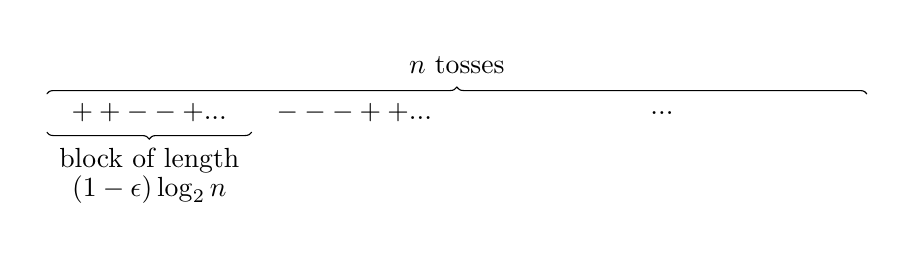
\begin{tikzpicture}
\begin{axis}[
width=12cm,height=4cm,
axis line style={draw=none},
xmin=0,xmax=2,
ymin=-0.1,ymax=0.4,
xticklabels=\empty,
yticklabels=\empty,
tick style={draw=none},
]
\node at (0.25,0.2) {$++--+...$};
\node at (0.75,0.2) {$---++...$};
\node at (1.5,0.2) {$...$};
\draw[decoration={brace,mirror},decorate] (0,0.15) -- (0.5,0.15);
\node at (0.25,0.075) {block of length};
\node at (0.25,0) {$(1-\epsilon)\log_2{n}$};
\draw[decoration={brace,mirror},decorate] (2,0.25) -- (0,0.25);
\node at (1,0.325) {$n$ tosses};
\end{axis}
\end{tikzpicture}\\
\textbf{Figure 10: Split $n$ tosses into separated blocks of length $(1-\epsilon)\log_2{n}$.}
\end{center}
Observe that, the probability of getting only heads in a given block is computed by,
\begin{center}
	$\mathbb{P}(\ell_{(1-\epsilon)\log_2{n}} = (1-\epsilon)\log_2{n}) = (\frac{1}{2})^{(1-\epsilon)\log_2{n}} = \frac{1}{n^{1-\epsilon}}$.
\end{center}
To this end, it is somewhat obvious that the probability of $L_n$ being less than $(1-\epsilon)\log_2{n}$ is bounded above by the probability of every block having least one $-1$, where we have a total of $\frac{n}{(1-\epsilon)\log_2{n}}$ independent blocks. Hence, we get that,
\begin{eqnarray}
\nonumber
\mathbb{P}(L_n < (1-\epsilon)\log_2{n}) &\leq& (1 - \mathbb{P}(\ell_{(1-\epsilon)\log_2{n}} = (1-\epsilon)\log_2{n}))^{\frac{n}{(1-\epsilon)\log_2{n}}}\\
\nonumber
&=& \left(1 - \frac{1}{n^{1-\epsilon}}\right)^{\frac{n}{(1-\epsilon)\log_2{n}}}\\
\nonumber
&\leq& e^{-\frac{1}{n^{1-\epsilon}}\frac{n}{(1-\epsilon)\log_2{n}}} \ \ \ \ \ \text{($1-x \leq e^{-x}$, for $x \geq 0$)}\\
\nonumber
&\leq& e^{-\frac{n^\epsilon}{\log_2{n}}}, \ \ \ \ \ \text{(by removing the exponent $\frac{1}{1-\epsilon}$)}
\end{eqnarray}
which yields,
\begin{center}
	$\sum_{n=1}^{\infty}\mathbb{P}(L_n < (1-\epsilon)\log_2{n}) \leq \sum_{n=1}^{\infty}e^{-\frac{n^\epsilon}{\log_2{n}}} < \infty$.
\end{center}
Thus, by Borel-Cantelli lemma (i), it follows that,
\begin{eqnarray}
\nonumber
\mathbb{P}(\{L_n < (1-\epsilon)\log_2{n} \ \text{i.o.}\}) = 0 &\iff& \mathbb{P}(\{L_n \geq (1-\epsilon)\log_2{n} \ \text{ev.}\}) = 1\\
\nonumber
&\iff& \exists n_\epsilon \geq 1 \ \text{such that} \ \forall m \geq n_\epsilon, \ \frac{L_m}{\log_2{m}} \geq 1-\epsilon\ \mathbb{P}\text{-a.s.}\\
\nonumber
&\xRightarrow{\epsilon \downarrow 0}& \liminf_{n\to\infty}\frac{L_n}{\log_2{n}} \geq 1 \ \mathbb{P}\text{-a.s.}.
\end{eqnarray}
We always have that,
\begin{eqnarray}
\nonumber
\liminf_{n\to\infty}\frac{L_n}{\log_2{n}} \leq \limsup_{n\to\infty}\frac{L_n}{\log_2{n}},
\end{eqnarray}
so we can deduce that,
\begin{eqnarray}
\nonumber
\limsup_{n\to\infty}\frac{L_n}{\log_2{n}} \leq 1 \leq \liminf_{n\to\infty}\frac{L_n}{\log_2{n}} \ \mathbb{P}\text{-a.s.}\iff \lim_{n\to\infty}\frac{L_n}{\log_2{n}} = 1 \ \mathbb{P}\text{-a.s.}.
\end{eqnarray}
Remarkably, this outcome is even stronger than that of Example 5.2.1. Not only the longest head run is substantially large infinitely many times, it is guaranteed that eventually, we always keep rolling heads.\\\\
In section 4.5, we examine convergence of sequences of Borel functions almost everywhere, in measure and in $\mathcal{L}^p$, for some $p \geq 1$. In the setting of $(\Omega,\mathcal{F},\mathbb{P})$ being a probability space and a sequence of Borel functions $(X_n)_{n\geq1}$, in which case is a sequence of real-valued random variables, we have the corresponding modes of convergence. Henceforth, by convention, we refer to ‘real-valued random variables’ as ‘random variables’.\\\\
\noindent\fbox{%
	\parbox{\textwidth}{%
		\textbf{Definition 5.2.2. Convergence $\mathbb{P}$-a.s.} \\ Let $(\Omega,\mathcal{F},\mathbb{P})$ be a probability space and $(X_n)_{n\geq1}, X$ be random variables. We say that, $(X_n)_{n\geq1}$ converges to $X$ $\mathbb{P}$-a.s., if and only if
		\begin{center}
			$\mathbb{P}(\{\lim_{n\to\infty}X_n = X\}^c) = 0$.
		\end{center}
		Then, we write $X_n \xrightarrow{\mathbb{P}\text{-a.s.}} X$.
	}%
}\\\\\\
\noindent\fbox{%
	\parbox{\textwidth}{%
		\textbf{Definition 5.2.3. Convergence in probability} \\ Let $(\Omega,\mathcal{F},\mathbb{P})$ be a probability space and $(X_n)_{n\geq1}, X$ be random variables. We say that, $(X_n)_{n\geq1}$ converges to $X$ in probability, if and only if $\forall \epsilon > 0$,
		\begin{center}
			$\lim_{n\to\infty}\mathbb{P}(|X_n - X| > \epsilon) = 0$.
		\end{center}
		Then, we write $X_n \xrightarrow{\mathbb{P}} X$.
	}%
}\\\\\\
\noindent\fbox{%
	\parbox{\textwidth}{%
		\textbf{Definition 5.2.4. Convergence in $\mathcal{L}^p$ or in $p^{th}$ moment} \\ Let $(\Omega,\mathcal{F},\mathbb{P})$ be a probability space and $(X_n)_{n\geq1}, X$ be random variables with $X \in \mathcal{L}^p(\mathbb{P}), \ p \in [1,\infty)$, i.e.
		\begin{center}
			$\mathbb{E}[|X|^p] = \int_\Omega |X|^p d\mathbb{P} < \infty$.
		\end{center}
		We say that, $(X_n)_{n\geq1}$ converges to $X$ in $\mathcal{L}^p$ or in $p^{th}$ moment, if and only if
		\begin{center}
			$\lim_{n\to\infty}\mathbb{E}[|X_n - X|^p] = 0$.
		\end{center}
		Then, we write $X_n \xrightarrow{\mathcal{L}^p} X$.
	}%
}\\\\\\
Recall that, a random variable $X$ on a probability space $(\Omega,\mathcal{F},\mathbb{P})$ is equipped with a distribution function $F_X(x) = \mathbb{P}(X \leq x), \ x\in\mathbb{R}$. In particular, we can discuss convergence of a sequence of random variables via their distribution functions.\\\\
\noindent\fbox{%
	\parbox{\textwidth}{%
		\textbf{Definition 5.2.5. Convergence in distribution} \\ Let $(\Omega,\mathcal{F},\mathbb{P})$ be a probability space and $(X_n)_{n\geq1}, X$ be random variables with $(F_{X_n})_{n\geq1}, F_X$ their corresponding distribution functions. We say that, $(X_n)_{n\geq1}$ converges to $X$ in distribution, if and only if
		\begin{center}
			$\lim_{n\to\infty}F_{X_n}(x) = F_X(x)$,
		\end{center}
		for every point $x\in\mathbb{R}$ at which $F_X$ is continuous. Then, we write $X_n \xrightarrow{\mathcal{D}} X$.
	}%
}\\\\\\
\textbf{Remark:} Convergence in distribution is only concerned with the associated distribution functions. More precisely, a sequence of random variables $(X_n)_{n\geq1}$ converging in distribution to some random variable $X$ might even be defined on a different probability space from that of $X$.\\\\
\textbf{Example 5.2.3.} Let $((H,T),\mathcal{P}(H,T),\mathbb{P})$ be a probability space, where $H$ and $T$ denote getting ‘heads’ and ‘tails’ from coin toss, respectively. Consider the sequence of random variables $(X_n)_{n\geq1}$ given by,
\begin{center}
	$X_n(\omega) = 
	\begin{cases}
	1, & \omega = T\\
	0, & \omega = H
	\end{cases}$
\end{center}
each with distribution function,
\begin{center}
	$F_{X_n}(x) = 
	\begin{cases}
	0, & x < 0 \\
	\frac{1}{2}, & 0 \leq x < 1 \\
	1, & x \geq 1
	\end{cases}$
\end{center}
The random variable $X$ defined by,
\begin{center}
	$X(\omega) = 
	\begin{cases}
	1, & \omega = H\\
	0, & \omega = T
	\end{cases}$
\end{center}
with distribution function,
\begin{center}
	$F_{X}(x) = 
	\begin{cases}
	0, & x < 0 \\
	\frac{1}{2}, & 0 \leq x < 1 \\
	1, & x \geq 1
	\end{cases}$
\end{center}
is different from each $X_n$, but clearly, it has the same distribution function as $X_n$ for every $x \in \mathbb{R}$, i.e. $X_n \neq X$, but $X_n \overset{\mathrm{\mathcal{D}}}{=} X$.\\\\
We shall later see that convergence in distribution is the weakest among these modes of convergence. However, it is quite often useful in practice.\\\\
In many cases, almost sure convergence can be relatively difficult to prove. Thus, we want to establish some sufficient conditions for almost sure convergence. Let $(X_n)_{n\geq1}$ be random variables on a probability space $(\Omega,\mathcal{F},\mathbb{P})$, such that $X_n \xrightarrow{\mathbb{P}\text{-a.s.}} X$. First, given $\epsilon > 0$ and $n \geq 1$, we define,
\begin{center}
	$B_n(\epsilon) = \{\omega\in\Omega: |X_n(\omega) - X(\omega)| \leq \epsilon\} = \{|X_n - X| \leq \epsilon\}$,
\end{center}
where $B_n(\epsilon)$ illustrates a ‘ball’ around $X$ by a distance at most $\epsilon$ from $X_n$. Then, we can write,
\begin{eqnarray}
\nonumber
\left\{\lim_{n\to\infty}X_n = X\right\} &=& \{\omega\in\Omega: \forall \epsilon>0, \ \exists n \geq 1 \ \text{such that} \ \forall m \geq n, \ |X_n(\omega) - X(\omega)| \leq \epsilon\}\\
\nonumber
&=& \bigcap_{\epsilon>0}\bigcup_{n=1}^{\infty}\bigcap_{m=n}^{\infty}B_m(\epsilon)\\
\nonumber
&=& \bigcap_{\epsilon>0}\liminf_{n\to\infty}B_n(\epsilon).
\end{eqnarray}
Set $\epsilon := \frac{1}{N}, \ \forall N \in \mathbb{N}$, so that,
\begin{eqnarray}
\nonumber
\bigcap_{\epsilon>0}\liminf_{n\to\infty}B_n(\epsilon) = \bigcap_{N=1}^{\infty}\liminf_{n\to\infty}B_n\left(\frac{1}{N}\right).
\end{eqnarray}
\noindent\fbox{%
	\parbox{\textwidth}{%
		\textbf{Proposition 5.2.1. Criterion for convergence $\mathbb{P}$-a.s.} \\ Let $(\Omega,\mathcal{F},\mathbb{P})$ be a probability space and $(X_n)_{n\geq1}, X$ be random variables. Then, $(X_n)_{n\geq1}$ converges to $X$ $\mathbb{P}$-a.s., if and only if
		\begin{center}
			$\lim_{N\to\infty}\mathbb{P}(\{|X_n - X| > \frac{1}{N} \ \text{i.o.}\}) = 0$.
		\end{center}
	}%
}\\\\\\
\textit{Proof.} Notice that, $B_n(\frac{1}{N})$ is decreasing in $N$, so by Continuity from above, we get that,
\begin{eqnarray}
\nonumber
1 = \mathbb{P}\left(\left\{\lim_{n\to\infty}X_n = X\right\}\right) &=& \mathbb{P}\left(\bigcap_{N=1}^{\infty}\liminf_{n\to\infty}B_n\left(\frac{1}{N}\right)\right)\\
\nonumber
&=& \lim_{N\to\infty}\mathbb{P}\left(\liminf_{n\to\infty}B_n\left(\frac{1}{N}\right)\right)\\
\nonumber
&=& \lim_{N\to\infty}\mathbb{P}\left(\left\{B_{n}\left(\frac{1}{N}\right) \ \text{ev.}\right\}\right).
\end{eqnarray}
Similarly, $B_n^c(\frac{1}{N}) = \{|X_n - X| > \frac{1}{N}\}$ is increasing in $N$, so by Continuity from below, we have that,
\begin{eqnarray}
\nonumber
0 = \mathbb{P}\left(\left\{\lim_{n\to\infty}X_n = X\right\}^c\right) &=& \mathbb{P}\left(\bigcup_{N=1}^{\infty}\limsup_{n\to\infty}B_n^c\left(\frac{1}{N}\right)\right)\\
\nonumber
&=& \lim_{N\to\infty}\mathbb{P}\left(\limsup_{n\to\infty}B_n^c\left(\frac{1}{N}\right)\right)\\
\nonumber
&=& \lim_{N\to\infty}\mathbb{P}\left(\left\{B_{n}^c\left(\frac{1}{N}\right) \ \text{i.o.}\right\}\right).
\end{eqnarray}
${}$ \hfill $\square$ \\\\
\textbf{Remarks:}
\begin{enumerate}
	\item For all sufficiently small $\epsilon > 0$, we can apply Borel-Cantelli lemma (i) to deduce almost sure convergence, that is, $\exists \delta>0$ such that $\forall \epsilon < \delta$,
	\begin{center}
		$\sum_{n=1}^{\infty}\mathbb{P}(B_n^c(\epsilon)) < \infty \implies \mathbb{P}(\{B_n^c(\epsilon) \ \text{i.o.}\}) = 0$,
	\end{center}
	thus $X_n \xrightarrow{\mathbb{P}\text{-a.s.}} X$.
	\item Conversely, if $(X_n)_{n\geq1}$ are independent and $X$ is constant, then by finding a sequence of sufficiently small $\epsilon > 0$, we can apply Borel-Cantelli lemma (ii) to argue that almost sure convergence does not hold, that is, $\forall \delta > 0, \exists \epsilon < \delta$ such that,
	\begin{center}
		$\sum_{n=1}^{\infty}\mathbb{P}(B_n^c(\epsilon)) = \infty \implies \mathbb{P}(\{B_n^c(\epsilon) \ \text{i.o.}\}) = 1 > 0$,
	\end{center}
	thus $X_n \overset{\mathrm{\mathbb{P}\text{-a.s.}}}{\nrightarrow} X$.
\end{enumerate}
\textbf{Example 5.2.4.} Let $(\Omega,\mathcal{F},\mathbb{P})$ be a probability space and $(X_n)_{n\geq1}$ be a sequence of independent identically distributed random variables, each uniformly distributed in $(0,1)$. Consider the sequence of random variables $(Y_n)_{n\geq1}$ given by,
\begin{center}
	$Y_n = \min\{X_1,...,X_n\}, \ n\geq1$.
\end{center}
We show that $Y_n \xrightarrow{\mathbb{P}\text{-a.s.}} 0$. Then, $\forall \epsilon \in (0,1)$, we have that,
\begin{eqnarray}
	\nonumber
	\mathbb{P}(B_n^c(\epsilon)) = \mathbb{P}(|Y_n| > \epsilon) &=& \mathbb{P}(X_1 > \epsilon,...,X_n > \epsilon)\\
	\nonumber
	&=& \mathbb{P}(X_1 > \epsilon)^n \ \ \ \ \ \text{(by independence of $X_1,...,X_n$)}\\
	\nonumber
	&=& (1-\epsilon)^n, \ \ \ \ \ \text{(since $X_1,...,X_n$ are identically distributed)}
\end{eqnarray}
and consequently, we get that,
\begin{eqnarray}
\nonumber
\sum_{n=1}^{\infty}\mathbb{P}(B_n^c(\epsilon)) = \sum_{n=1}^{\infty}(1-\epsilon)^n = \frac{1-\epsilon}{\epsilon} < \infty.
\end{eqnarray}
Hence, $\forall \epsilon\in(0,1)$, by Borel-Cantelli lemma (i), it follows that,
\begin{eqnarray}
\nonumber
\mathbb{P}(\{B_n^c(\epsilon) \ \text{i.o.}\}) = \mathbb{P}(\{|Y_n| > \epsilon \ \text{i.o.}\}) = 0,
\end{eqnarray}
so that indeed, $Y_n \xrightarrow{\mathbb{P}\text{-a.s.}} 0$.
\begin{center}
	\noindent\rule{12cm}{0.4pt}
\end{center}
\textbf{Exercise 5.2.1.} Let $(\Omega,\mathcal{F},\mathbb{P})$ be a probability space and $(X_n)_{n\geq1}$ be a sequence of random variables with probability distribution given by,
\begin{center}
	$\mathbb{P}(X_n = 1) = p_n$ and $\mathbb{P}(X_n = 0) = 1 - p_n, \ n\geq1$.
\end{center}
Suppose also that, $\sum_{n=1}^{\infty}p_n < \infty$. Show that $X_n \xrightarrow{\mathbb{P}\text{-a.s.}} 0$.\\\\
\textit{Solution.} Notice that, $\forall \epsilon \in (0,1)$,
\begin{eqnarray}
\nonumber
\sum_{n=1}^{\infty}\mathbb{P}(B_n^c(\epsilon)) = \sum_{n=1}^{\infty}\mathbb{P}(|X_n| > \epsilon) = \sum_{n=1}^{\infty}\mathbb{P}(X_n = 1) = \sum_{n=1}^{\infty}p_n < \infty.
\end{eqnarray}
Therefore, by Borel-Cantelli lemma (i), we get that,
\begin{eqnarray}
\nonumber
\mathbb{P}(\{B_n^c(\epsilon) \ \text{i.o.}\}) = \mathbb{P}(\{|X_n| > \epsilon \ \text{i.o.}\}) = 0,
\end{eqnarray}
thus, $X_n \xrightarrow{\mathbb{P}\text{-a.s.}} 0$.\\\\
\textbf{Exercise 5.2.2.} Let $(\Omega,\mathcal{F},\mathbb{P})$ be a probability space and $X$ a continuous random variable, such that $\mathbb{P}(|X| < \infty) = 1$. Consider the sequence of random variables $(X_n)_{n\geq1}$, where $X_n = \frac{n}{n+1}X, \ n\geq1$. Verify that $X_n \xrightarrow{\mathbb{P}\text{-a.s.}} X$.\\\\
\textit{Solution.} One way to show this is by splitting the associated infinite series and then apply Borel-Cantelli lemmas. Using the fact that $|X|$ is continuous and finite $\mathbb{P}$-almost surely, we can see that,
\begin{eqnarray}
\nonumber
\forall \epsilon > 0, \ \exists N \in \mathbb{N} \ \text{such that} \ \forall n \geq N, \ \mathbb{P}(|X_n - X| > \epsilon) = \mathbb{P}(|X| > \epsilon(n+1)) = 0 \ \mathbb{P}\text{-a.s.}.
\end{eqnarray}
Hence, we get that,
\begin{eqnarray}
\nonumber
\sum_{n=1}^{\infty}\mathbb{P}(|X_n - X| > \epsilon) = \sum_{n=1}^{N}\mathbb{P}(|X_n - X| > \epsilon) + \sum_{n=N+1}^{\infty}\mathbb{P}(|X_n - X| > \epsilon) < \infty,
\end{eqnarray}
since the first quantity is a finite sum and the second follows from the previous assertion. Thus, by Borel-Cantelli lemma (i), it follows that,
\begin{eqnarray}
\nonumber
\mathbb{P}(\{|X_n - X| > \epsilon \ \text{i.o.}\}) = 0,
\end{eqnarray}
so that indeed, $X_n \xrightarrow{\mathbb{P}\text{-a.s.}} X$.
\begin{center}
	\noindent\rule{12cm}{0.4pt}
\end{center}
When applying Borel-Cantelli lemma (ii), we must be careful that the necessary conditions are met, especially independence of random variables.\\\\
\textbf{Example 5.2.5.} Let $(\Omega,\mathcal{F},\mathbb{P})$ be a probability space and $(X_n)_{n\geq1}$ be a sequence of random variables that forms a discrete-time Markov chain, which is $\{0,1\}$-valued, that is,
\begin{center}
	$\mathbb{P}(X_{n+1} = 1| X_n = 1) = \frac{n}{n+1}$ and $\mathbb{P}(X_{n+1} = 0| X_n = 0) = 1$.
\end{center}
We can easily compute that,
\begin{center}
	$\mathbb{P}(X_{n+1} = 0| X_n = 1) = \frac{1}{n+1}$ and $\mathbb{P}(X_{n+1} = 1| X_n = 0) = 0$.
\end{center}
We want to check whether $X_n \xrightarrow{\mathbb{P}\text{-a.s.}} 0$ or not. Starting from $X_1 = 1$, we can either be at state $1$ at time $2$ with probability $\frac{1}{2}$, or visit $0$ with probability $\frac{1}{2}$ and stay there forever. If the former case happens, we can either be at state $1$ at time $3$ with probability $\frac{2}{3}$, or visit $0$ with probability $\frac{1}{3}$ and stay there forever. We can similarly argue at any point in time, so we can see that the probability of reaching $0$ is decreasing in time. However, there is always some small probability, so our intuition should tell us that eventually, we are at state $0$. Let us first approach this problem using Borel-Cantelli lemmas. One result that follows from construction of this Markov chain is the following:
\begin{center}
	$\mathbb{P}(X_m = 0| X_n = 0) = 1, \ \forall m > n$. \ \ \ \ \ $(*)$
\end{center}
Indeed, observe that,
\begin{eqnarray}
	\nonumber
	\mathbb{P}(X_{n+1} = 0| X_n = 0) &=& 1,\\
	\nonumber
	\mathbb{P}(X_{n+2} = 0| X_n = 0) &=& \mathbb{P}(X_{n+2} = 0, X_{n+1} = 0| X_n = 0) + \mathbb{P}(X_{n+2} = 0, X_{n+1} = 1| X_n = 0)\\
	\nonumber
	&=& \mathbb{P}(X_{n+2} = 0| X_{n+1} = 0, X_n = 0)\mathbb{P}(X_{n+1} = 0| X_n = 0) \\
	\nonumber
	&{}& + \mathbb{P}(X_{n+2} = 0| X_{n+1} = 1, X_n = 0)\mathbb{P}(X_{n+1} = 1| X_n = 0)\\
	\nonumber
	&=& \mathbb{P}(X_{n+2} = 0| X_{n+1} = 0)\mathbb{P}(X_{n+1} = 0| X_n = 0) \\
	\nonumber
	&{}& + \mathbb{P}(X_{n+2} = 0| X_{n+1} = 1)\mathbb{P}(X_{n+1} = 1| X_n = 0) \ \ \ \ \ \text{(by the Markov property)}\\
	\nonumber
	&=& 1.
\end{eqnarray}
Proceed by induction to get the result. This in turn implies that, $\forall \epsilon \in (0,1)$,
\begin{eqnarray}
\nonumber
\mathbb{P}(B_n^c(\epsilon)) &=& \mathbb{P}(|X_n| > \epsilon) \\
\nonumber
&=& \mathbb{P}(X_n = 1) \\
\nonumber
&=& \mathbb{P}(X_n = ... = X_1 = 1) \ \ \ \ \ \text{(by $(*)$)}\\
\nonumber
&=& \mathbb{P}(X_n = 1| X_{n-1} = 1) \ ... \ \mathbb{P}(X_2 = 1| X_1 = 1) \ \ \ \ \ \text{(by the Markov proparty)}\\
\nonumber
&=& \frac{n-1}{n}\frac{n-2}{n-1} \ ... \ \frac{1}{2} = \frac{1}{n},
\end{eqnarray}
which then yields,
\begin{eqnarray}
\nonumber
\sum_{n=1}^{\infty}\mathbb{P}(B_n^c(\epsilon)) = \sum_{n=1}^{\infty}\mathbb{P}(X_n = 1) = \sum_{n=1}^{\infty}\frac{1}{n} = \infty.
\end{eqnarray}
However, we cannot apply Borel-Cantelli lemma (ii) to deduce that almost sure convergence to $0$ does not hold, unless $(X_n)_{n\geq1}$ are independent. But, this is not the case here, precisely by the Markov property, in which case $(X_n)_{n\geq1}$ are strongly dependent. Thereby, notice that,
\begin{eqnarray}
\nonumber
\mathbb{P}(\{\lim_{n\to\infty}X_n = 0\}^c) &=& \mathbb{P}(\lim_{n\to\infty}X_n = 1) = \mathbb{P}(X_1 = X_2 = ... = 1)\\
\nonumber
&\leq& \mathbb{P}(X_1 = ... = X_m = 1) = \frac{1}{m}, \ \forall m \in \mathbb{N} \xrightarrow{m\to\infty} 0,
\end{eqnarray}
where we exploit precisely the underlying intuition of this two-state Markov chain, so that indeed, $X_n \xrightarrow{\mathbb{P}\text{-a.s.}} 0$. \\\\
Recall Lemma 4.5.3, where in a probability space, we establish that convergence in $\mathcal{L}^p$ implies convergence in probability, by Chebyshev's inequality. In fact, almost sure convergence also implies convergence in probability. A sequence of random variables $(X_n)_{n\geq1}$ on a probability space $(\Omega,\mathcal{F},\mathbb{P})$ converges in probability to a random variable $X$, if and only if, $\forall \epsilon > 0$,
\begin{center}
	$\lim_{n\to\infty}\mathbb{P}(|X_n - X| > \epsilon) = \lim_{n\to\infty}\mathbb{P}(B_n^c(\epsilon)) = 0$,
\end{center}
where as usual, $B_n^c(\epsilon) = \{|X_n - X| > \epsilon\}$. We prove our assertion through the proposition below.\\\\
\noindent\fbox{%
	\parbox{\textwidth}{%
		\textbf{Proposition 5.2.2. Convergence $\mathbb{P}$-a.s. implies convergence in probability} \\ Let $(\Omega,\mathcal{F},\mathbb{P})$ be a probability space and $(X_n)_{n\geq1}, X$ be random variables. Then,
		\begin{center}
			$X_n \xrightarrow{\mathbb{P}\text{-a.s.}} X \implies X_n \xrightarrow{\mathbb{P}} X$.
		\end{center}
	}%
}\\\\\\
\textit{Proof.} Since $X_n \xrightarrow{\mathbb{P}\text{-a.s.}} X$, then for all sufficiently small $\epsilon > 0$, 
\begin{eqnarray}
\nonumber
0 &=& \mathbb{P}(\{B_n^c(\epsilon) \ \text{i.o.}\})\\
\nonumber
&=& \mathbb{P}\left(\bigcap_{n=1}^{\infty}\bigcup_{m=n}^{\infty}B_m^c(\epsilon)\right)\\
\nonumber
&=& \lim_{n\to\infty}\mathbb{P}\left(\bigcup_{m=n}^{\infty}B_m^c(\epsilon)\right). \ \ \ \ \ \text{(by Continuity from above)}
\end{eqnarray}
Now, it is clear that, $B_n^c(\epsilon) \subseteq \bigcup_{m=n}^{\infty}B_m^c(\epsilon), \ \forall n \geq 1$. Hence, by monotonicity of (probability) measures, it follows that,
\begin{eqnarray}
\nonumber
\mathbb{P}(B_n^c(\epsilon)) \leq \mathbb{P}\left(\bigcup_{m=n}^{\infty}B_m^c(\epsilon)\right) \xRightarrow{n\to\infty} \lim_{n\to\infty}\mathbb{P}(B_n^c(\epsilon)) \leq \lim_{n\to\infty}\mathbb{P}\left(\bigcup_{m=n}^{\infty}B_m^c(\epsilon)\right) = 0,
\end{eqnarray}
which implies that, $X_n \xrightarrow{\mathbb{P}} X$. \\
${}$ \hfill $\square$ \\\\
\textbf{Remark:} In Example 4.5.1, the traveling wave converges $m$-almost everywhere, but neither in measure nor in $\mathcal{L}^p$. We would expect that convergence $m$-almost everywhere implies convergence in measure, as in a probability space, but it fails in this case. This is because the Lebesgue measure $m$ is an infinite measure, i.e. $m(\mathbb{R}) = \infty$, whereas a probability measure is bounded above by $1$. In fact, if $(f_n)_{n\geq1}$ is a sequence of Borel functions on a given measure space $(\Omega,\mathcal{F},\mu)$, where $\mu(\Omega) < \infty$, which converges $\mu$-almost everywhere to a Borel function $f$, then it also converges in measure to $f$. \\\\
Convergence in distribution is actually the weakest concept, so it is implied by all modes of convergence. Then, the following diagram summarizes the relationship arising between the four different notions of convergence:
\begin{eqnarray}
	\nonumber
	\text{convergence} \ \mathbb{P}\text{-a.s.} &\text{\begin{turn}{-30} $\implies$ \end{turn}}&\\
	\nonumber
	&{}& \text{convergence in probability} \implies \text{convergence in distribution}\\
	\nonumber
	\text{convergence in} \ \mathcal{L}^p &\text{\begin{turn}{30} $\implies$ \end{turn}}&
\end{eqnarray}
Thus, it suffices to show that convergence in probability implies convergence in distribution.\\\\
\noindent\fbox{%
	\parbox{\textwidth}{%
		\textbf{Proposition 5.2.3. Convergence in probability implies convergence in distribution} \\ Let $(\Omega,\mathcal{F},\mathbb{P})$ be a probability space and $(X_n)_{n\geq1}, X$ be random variables. Then,
		\begin{center}
			$X_n \xrightarrow{\mathbb{P}} X \implies X_n \xrightarrow{\mathcal{D}} X$.
		\end{center}
	}%
}\\\\\\
\textit{Proof.} By elementary set operations, we can write, $\forall a \in \mathbb{R}$,
\begin{eqnarray}
\nonumber
\{X_n \leq a\} &=& \{X_n \leq a, X \leq a+\epsilon\}\cup\{X_n \leq a, X > a+\epsilon\} \subseteq \{X \leq a+\epsilon\}\cup\{|X_n - X| > \epsilon\},\\
\nonumber
\{X \leq a-\epsilon\} &=& \{X \leq a-\epsilon, X_n \leq a\}\cup\{X \leq a-\epsilon, X_n > \alpha\} \subseteq \{X_n \leq a\}\cup\{|X_n - X| > \epsilon\}.
\end{eqnarray}
By countable additivity and monotonicity of $\mathbb{P}$, we have that,
\begin{eqnarray}
\nonumber
\mathbb{P}(X_n \leq a) &\leq& \mathbb{P}(X \leq a+\epsilon) + \mathbb{P}(|X_n - X| > \epsilon),\\
\nonumber
\mathbb{P}(X \leq a-\epsilon) &\leq& \mathbb{P}(X_n \leq a) + \mathbb{P}(|X_n - X| > \epsilon).
\end{eqnarray}
Now, taking limit superior and limit inferior respectively, yields,
\begin{eqnarray}
\nonumber
\limsup_{n\to\infty}\mathbb{P}(X_n \leq a) &\leq& \mathbb{P}(X \leq a+\epsilon),\\
\nonumber
\mathbb{P}(X \leq a-\epsilon) &\leq& \liminf_{n\to\infty}\mathbb{P}(X_n \leq a),
\end{eqnarray}
where we use the fact that,
\begin{eqnarray}
\nonumber
\limsup_{n\to\infty}\mathbb{P}(|X_n - X| > \epsilon) = \liminf_{n\to\infty}\mathbb{P}(|X_n - X| > \epsilon) = \lim_{n\to\infty}\mathbb{P}(|X_n - X| > \epsilon) = 0.
\end{eqnarray}
For every point $a\in\mathbb{R}$ at which $F_X$ is continuous, we can take limit as $\epsilon \downarrow 0$, so that,
\begin{eqnarray}
\nonumber
\limsup_{n\to\infty}\mathbb{P}(X_n \leq a) \leq \mathbb{P}(X \leq a) \leq \liminf_{n\to\infty}\mathbb{P}(X_n \leq a) \iff \lim_{n\to\infty}\mathbb{P}(X_n \leq a) = \mathbb{P}(X \leq a),
\end{eqnarray}
and consequently, $X_n \xrightarrow{\mathcal{D}} X$.\\
${}$ \hfill $\square$\\\\
\textbf{Example 5.2.6.} Let $(\Omega,\mathcal{F},\mathbb{P})$ be a probability space and $(X_n)_{n\geq1}$ be a sequence of random variables, each Cauchy distributed with location parameter $0$ and scale parameter $\frac{1}{n}$, that is,
\begin{center}
	$f_n(x) = \frac{1}{\frac{1}{n}\pi(1 + n^2x^2)} = \frac{n}{\pi(1+n^2x^2)}, \ x \in \mathbb{R}, \ n \geq 1$.
\end{center}
From Figure 11, we can see that as $n$ gets larger, $f_n(x)$ becomes closer to $f(x) = 0$, so we claim that $X_n$ converges in distribution to $0$.
\begin{center}
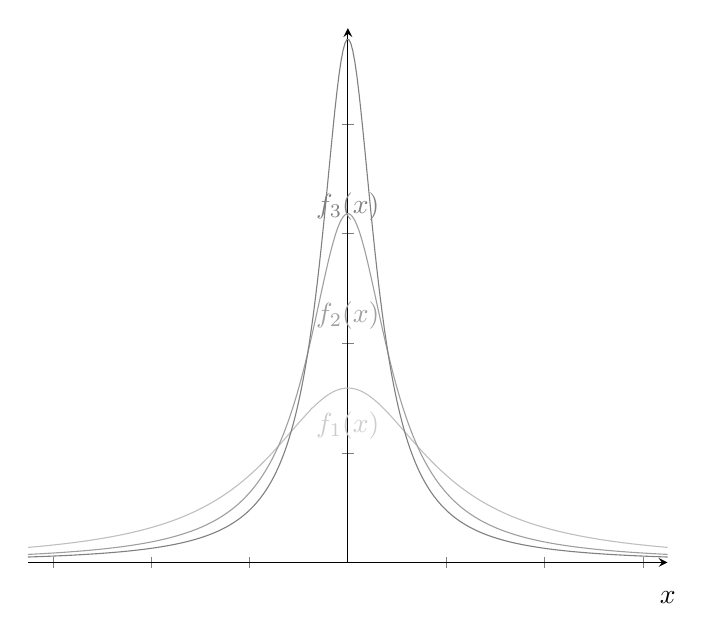
\begin{tikzpicture}
\begin{axis}[
width=0.8\textwidth,
axis lines = middle,
x label style={at={(current axis.right of origin)},anchor=north, below=2.5mm},
xlabel = {$x$},
xmin=-3.25,xmax=3.25,
ymin=0,ymax=0.975,
yticklabels=\empty,
xticklabels=\empty,
]
\node[gray] at (0,0.65) {$f_3(x)$};
\node[gray!75] at (0,0.45) {$f_2(x)$};
\node[gray!40] at (0,0.25) {$f_1(x)$};
\addplot[color=gray!50, domain=-10:10,samples=1000] {1/(pi*(1 + 1^2*x^2))};
\addplot[color=gray!75, domain=-10:10,samples=1000] {2/(pi*(1 + 2^2*x^2))};
\addplot[color=gray, domain=-10:10,samples=1000] {3/(pi*(1 + 3^2*x^2))};
\end{axis}
\end{tikzpicture}\\
\textbf{Figure 11: Probability density function of Cauchy distribution with location parameter $0$ and scale parameter $n = 1,\frac{1}{2},\frac{1}{3}$.}
\end{center}
We have that, $\forall \epsilon > 0$,
\begin{eqnarray}
\nonumber
\mathbb{P}(|X_n| > \epsilon) = \int_\epsilon^\infty \frac{n}{\pi(1 + n^2x^2)} dm = \left[\frac{\arctan(nx)}{\pi}\right]_{\epsilon}^{\infty} = \frac{1}{2} - \frac{\arctan(n\epsilon)}{\pi} \xRightarrow{n\to\infty} \lim_{n\to\infty}\mathbb{P}(|X_n|>\epsilon) = 0,
\end{eqnarray}
thus, $X_n \xrightarrow{\mathbb{P}} 0$, and by Proposition 5.2.3, $X_n \xrightarrow{\mathcal{D}} 0$.\\\\
Unsurprisingly, convergence in distribution can be determined by the moment generating functions of the corresponding sequence of random variables, assuming that they exist on some interval. Known as Levy's Convergence Theorem, this result is critical for proving the Central Limit Theorem.\\\\
\noindent\fbox{%
	\parbox{\textwidth}{%
		\textbf{Theorem 5.2.1. Levy's Convergence Theorem} \\ Let $(\Omega,\mathcal{F},\mathbb{P})$ be a probability space and $(X_n)_{n\geq1}, X$ be random variables with $(M_{X_n})_{n\geq1}, M_X$ their corresponding moment generating functions, which exist on $t \in (-h,h)$, for some $h \in \mathbb{R}$. Then,
		\begin{center}
			$\lim_{n\to\infty}M_{X_n}(t) = M_X(t), \ \forall t < |h| \implies X_n \xrightarrow{\mathcal{D}} X$.
		\end{center}
	}%
}\\\\\\
\textbf{Remark:} This theorem can be extended to pointwise convergence of any characteristic functions $\phi_{X_n}(t) = \mathbb{E}[e^{itX_n}]$, which indicate the Laplace transform with complex variables of the corresponding probability density functions $f_{X_n}(x)$, $n \geq 1$. By uniqueness of the Laplace transform, characteristic functions provide an alternative way of obtaining insightful results. However, the underlying theory is beyond the scope of this module and we restrict our interest to the special case of moment generating functions $\phi_{X_n}(-it) = M_{X_n}(t)$.\\\\
\textbf{Example 5.2.7.} Let $(\Omega,\mathcal{F},\mathbb{P})$ be a probability space and $(Y_n)_{n\geq1}$ be a sequence of independent random variables, each with probability distribution given by,
\begin{center}
	$\mathbb{P}(Y_n = j) = \frac{1}{10}, \ n\geq1, \ j = 0,1,...,9$.
\end{center}
Consider the sequence of random variables $(X_n)_{n\geq1}$ given by,
\begin{center}
	$X_n = \sum_{i=1}^{n}\frac{Y_i}{10^i}, \ n\geq1$,
\end{center}
which represents a number in $(0,1)$ with $Y_i$ as the $i^{th}$ digit, $i=1,...,n$. We are interested in the limiting distribution of $(X_n)_{n\geq1}$, which we uncover by the corresponding moment generating functions $(M_{X_n})_{n\geq1}$. Then, we have that,
\begin{eqnarray}
\nonumber
M_{X_n}(t) = \mathbb{E}[e^{tX_n}] = \mathbb{E}[e^{t\sum_{i=1}^{n}\frac{Y_i}{10^i}}] = \prod_{i=1}^{n}\mathbb{E}[e^{t\frac{Y_i}{10^i}}],
\end{eqnarray}
using the fact that $Y_1,...,Y_n$ are independent. Now, since $Y_i, \ i=1,...,n$, is a discrete random variable with distribution given as above, we get that,
\begin{eqnarray}
\nonumber
\mathbb{E}[e^{t\frac{Y_i}{10^i}}] = \sum_{j=0}^{9}e^{t\frac{j}{10^i}}\mathbb{P}(Y_i = j) = \frac{1}{10}(1 + e^{\frac{t}{10^i}} + ... + e^{\frac{9t}{10^i}}) = \frac{1}{10}\frac{1-e^{\frac{t}{10^{i-1}}}}{1-e^{\frac{t}{10^{i}}}}.
\end{eqnarray}
Thus, it follows that,
\begin{eqnarray}
\nonumber
M_{X_n}(t) = \frac{1}{10^n}\prod_{i=1}^{n}\frac{1-e^{\frac{t}{10^{i-1}}}}{1-e^{\frac{t}{10^{i}}}} = \frac{1}{10^n}\frac{1-e^t}{1-e^{\frac{t}{10^2}}}\frac{1-e^{\frac{t}{10^2}}}{1-e^{\frac{t}{10^3}}} \ ... \ \frac{1-e^{\frac{t}{10^{n-1}}}}{1-e^{\frac{t}{10^n}}} = \frac{1}{10^n}\frac{1-e^t}{1-e^{\frac{t}{10^n}}}.
\end{eqnarray}
To this end, by applying the limits given by,
\begin{eqnarray}
\nonumber
\lim_{x \to 0}\frac{x}{1-e^x} = -1 = \lim_{x\to\infty}\frac{\frac{1}{x}}{1-e^{\frac{1}{x}}},
\end{eqnarray}
we multiply both the numerator and denominator of $M_{X_n}(t)$ by $t$, so as to get,
\begin{eqnarray}
\nonumber
M_{X_n}(t) = \frac{\frac{t}{10^n}}{1-e^{\frac{t}{10^n}}}\frac{1-e^t}{t} \xrightarrow{n\to\infty} -\frac{1-e^t}{t},
\end{eqnarray}
which is precisely the moment generating function $M_X(t)$ of a uniformly distributed random variable $X$ on $(0,1)$. Indeed, we have that,
\begin{eqnarray}
\nonumber
M_X(t) = \int_{\mathbb{R}}e^{tx}\mathds{1}_{[0,1]}dm = \int_0^{1}e^{tx}dm = \left[\frac{e^{tx}}{t}\right]_{0}^{1} = \frac{e^t - 1}{t}.
\end{eqnarray}
Therefore, by Levy's Convergence theorem, $X_n \xrightarrow{\mathcal{D}} X \sim Uniform(0,1)$. This outcome is to be anticipated by construction of this experiment. Drawing $n$ digits independently and placing them in order with equal probability as $n$ gets larger, it gives any possible number in $(0,1)$ randomly, which crucially behaves as a $Uniform(0,1)$ distribution.
\subsection{Law of Large Numbers}
Under certain conditions, the Law of Large Numbers states that the empirical (sample) mean, after a large number of trials, approximates well the theoretical (population) mean. To motivate its importance, we use the Monte Carlo method in a probabilistic interpretation, which relies on random sampling repetitively to compute a deterministic quantity.\\\\
\textbf{Example 5.3.1.} Let $(\Omega,\mathcal{F},\mathbb{P})$ be a probability space. Our experiment aims in computing the number $\pi$, which exploits the Monte Carlo method and essentially, the Law of Large Numbers. The algorithm is given as follows:
\begin{enumerate}
	\item Inscribe a unit circle within a square, whose sides are of length $2$, as seen in Figure 12.
	\begin{center}
	\begin{tikzpicture}
	\draw (0,0) rectangle ++(7,7);
	\draw (7,3.5) arc (0:360:3.5);
	\node at (0,-0.35) {$-1$};
	\node at (-0.35,0) {$-1$};
	\node at (7,-0.35) {$1$};
	\node at (-0.35,7) {$1$};
	\draw[loosely dashed] (0,3.5) -- (7,3.5);
	\draw[loosely dashed] (3.5,0) -- (3.5,7);
	\node at (3.25,3.25) {$0$};
	\end{tikzpicture}\\
	\textbf{Figure 12: Approximating $\pi$ using the Monte Carlo method.}
	\end{center}
	\item Generate $n$ inputs from independent random variables $U,V \sim Uniform(-1,1)$ and place them across the square.
	\item For any input $i \in \{1,...,n\}$ that lies within the unit circle, that is, $U_i^2 + V_i^2 \leq 1$, set $X_i := 1$, otherwise set $X_i := 0$. Notice that, $\{X_i\}_{i=1}^{n}$ is a sequence of Bernoulli trials, where the expected value of each $X_i$ is equal to the theoretical probability of success $\frac{\pi}{4}\in(0,1)$, i.e. $\mathbb{E}[X_i] = \mathbb{P}(X_i = 1) = \frac{\pi}{4}$ is the ratio between the two shapes.
	\item The sample mean $\overline{X}_n := \frac{X_1 + ... + X_n}{n}$ becomes (nearly) deterministic and provides a good approximation for $\frac{\pi}{4}$, when $n$ is substantially large. Multiply by $4$ to get an approximation for $\pi$.
\end{enumerate}
In fact, there are two different versions of the Law of Large Numbers, with the first one stated below.\\\\
\noindent\fbox{%
	\parbox{\textwidth}{%
		\textbf{Theorem 5.3.1. Weak Law of Large Numbers (WLLN)} \\ Let $(\Omega,\mathcal{F},\mathbb{P})$ be a probability space and $(X_n)_{n\geq1}$ be a sequence of uncorrelated random variables, i.e. $\mathbb{E}[X_iX_j] = \mathbb{E}[X_i]\mathbb{E}[X_j], \ \forall i \neq j$, that are Lebesgue-integrable with $\mathbb{E}[X_i] = \mu$ and $Var(X_i) \leq C < \infty$, for some $C \in (0,\infty), \ \forall i \geq 1$. Then,
		\begin{center}
			$\overline{X}_n = \frac{1}{n}\sum_{i=1}^{n} X_i \xrightarrow{\mathbb{P}} \mu$,
		\end{center}
		that is $\forall \epsilon > 0$,
		\begin{center}
			$\lim_{n\to\infty}\mathbb{P}(|\overline{X}_n - \mu| > \epsilon) = 0$.
		\end{center}
	}%
}\\\\\\
\textit{Proof.} By linearity of expectation and the fact that $(X_n)_{n\geq1}$ are uncorrelated, we get that,
\begin{eqnarray}
\nonumber
\mathbb{E}[\overline{X}_n] &=& \mathbb{E}\left[\frac{1}{n}\sum_{i=1}^{n}X_i\right] = \frac{1}{n}\sum_{i=1}^{n}\mathbb{E}[X_i] = \mu,\\
\nonumber
Var(\overline{X}_n) &=& Var\left(\frac{1}{n}\sum_{i=1}^{n}X_i\right) = \frac{1}{n^2}\sum_{i=1}^{n}Var(X_i) \leq \frac{C}{n} \xrightarrow{n\to\infty} 0.
\end{eqnarray}
Now, applying Markov's inequality yields,
\begin{eqnarray}
\nonumber
\mathbb{P}(|\overline{X}_n - \mu| > \epsilon) = \mathbb{P}(|\overline{X}_n - \mathbb{E}[\overline{X}_n]| > \epsilon) \leq \frac{1}{\epsilon^2}Var({\overline{X}_n}) \xrightarrow{n\to\infty} 0,
\end{eqnarray}
which in turn implies that, $\overline{X}_n \xrightarrow{\mathbb{P}} \mu$.\\
${}$ \hfill $\square$ \\\\
\textbf{Remark:} The given assumptions are quite general and make the proof easy. The theorem might be seen in the settings of $(X_n)_{n\geq1}$ being independent identically distributed with $\mathbb{E}[X_1] = \mu$ and $\mathbb{E}[X_1^2] < \infty$. More generally, the second moment need not be finite, so we can require only $\mathbb{E}[|X_1|] < \infty$.\\\\
As in the proof of Theorem 5.3.1, Markov's inequality is quite helpful as it acts as an upper bound for deviation of the sample mean from the theoretical mean.\\\\
\textbf{Example 5.3.2.} Let $((H,T),\mathcal{P}(H,T),\mathbb{P})$ be a probability space and $\{X_i\}_{i=1}^{100}$ be a sequence of random variables defined by,
\begin{center}
	$X_i(\omega) = 
	\begin{cases}
	1, & \omega = H\\
	0, & \omega = T
	\end{cases}$
\end{center}
with probability distribution given by,
\begin{center}
	$\mathbb{P}(X_i = 1) = \mathbb{P}(X_i = 0) = \frac{1}{2}, \ i = 1,...,n$,
\end{center}
indicating fair coin tossing. First, the expectation and variance of the sample mean are computed by,
\begin{eqnarray}
\nonumber
\mathbb{E}[\overline{X}_{100}] &=& \mathbb{E}\left[\frac{1}{100}\sum_{i=1}^{100}X_i\right]= \frac{1}{2},\\
\nonumber
Var(\overline{X}_{100}) &=& Var\left(\frac{1}{100}\sum_{i=1}^{100}X_i\right) = \frac{\frac{1}{2}(1-\frac{1}{2})}{100} = \frac{\frac{1}{4}}{100}.
\end{eqnarray}
We want to compute the probability that the number of heads scored lies between $40$ and $60$, that is,
\begin{eqnarray}
\nonumber
\mathbb{P}\left(40 \leq \sum_{i=1}^{100}X_i \leq 60\right) &=& \mathbb{P}\left(\left|\overline{X}_{100} - \frac{1}{2}\right| \leq 0.1\right)\\
\nonumber
&=& 1 - \mathbb{P}\left(\left|\overline{X}_{100} - \frac{1}{2}\right| > \frac{1}{10}\right)\\
\nonumber
&\geq& 1 - \frac{1}{(\frac{1}{10})^2}Var(\overline{X}_{100}) \\
\nonumber
&=& 1 - 100\frac{\frac{1}{4}}{100} = \frac{3}{4},
\end{eqnarray}
which follows by applying Markov's inequality. This leads to the notion of confidence intervals.\\\\
Informally, given a probability space $(\Omega,\mathcal{F},\mathbb{P})$ and a sequence of independent identically distributed random variables $(X_n)_{n\geq1}$, a confidence interval for the theoretical mean $\mu = \mathbb{E}[X_1]$ is a random interval with accuracy $\epsilon > 0$ and confidence coefficient $\beta\%, \ \beta \in (0,100)$, such that
\begin{center}
	$\mathbb{P}(\mu \in (\overline{X}_{n} - \epsilon, \overline{X}_{n} + \epsilon)) \geq \frac{\beta}{100}$. 
\end{center}
\textbf{Example 5.3.1. (continued)} After getting an idea of how to approximate $\pi$, it makes sense to question what is an acceptable number $n$ of trials under certain accuracy and confidence coefficient. In particular, we require an accuracy of four digits, that is $\epsilon = \frac{1}{4000}$, and $99\%$ confidence coefficient. Then, applying again Markov's inequality yields,
\begin{eqnarray}
\nonumber
\mathbb{P}\left(\left|\overline{X}_n - \frac{\pi}{4}\right| > \frac{1}{4000}\right) \leq 4000^2 Var(\overline{X}_n) = 4000^2\frac{\frac{\pi}{4}(1-\frac{\pi}{4})}{n} \leq 0.01.
\end{eqnarray}
Now, using the fact that $\frac{\pi}{4}\in(0,1)$ and that,
\begin{center}
	$x(1-x) \leq \frac{1}{4}, \ \forall x \in [0,1]$,
\end{center}
it follows that,
\begin{eqnarray}
\nonumber
\mathbb{P}\left(\left|\overline{X}_n - \frac{\pi}{4}\right| > \frac{1}{4000}\right) \leq 4000^2\frac{1}{4n} \leq 0.01,
\end{eqnarray}
so that any number of trials $n \geq 400\times10^6$ gives $\frac{\pi}{4}$ with four-digit accuracy and $99\%$ confidence coefficient.\\\\
\textbf{Example 5.3.3.} Let $(\Omega,\mathcal{F},\mathbb{P})$ be a probability space and $(Y_n)_{n\geq1}$ be a sequence of independent identically distributed random variables, each uniformly distributed on $(-1,1)$. Consider the sequence of random variables $(X_n)_{n\geq1}$ given by,
\begin{center}
	$X_n = (Y_1,...,Y_n), \ n\geq1$,
\end{center}
which takes values uniformly on $(-1,1)^n$. Take for instance $n=2$ and $n=3$, where $X_2$ and $X_3$ represent square and cube, whose sides have length $2$, respectively. In fact, for substantially large $n$, $X_n$ becomes similar to a ‘high-dimensional sphere’. First, note that the area and volume of $X_2$ and $X_3$ are equal to $4$ and $8$. The generalised content increases exponentially with $n$ and is equal to $2^n$. This illustrates the idea that the distance from the origin of any point $x = (y_1,...,y_n) \in X_n$ depends on $n$, and is given by,
\begin{center}
	$|x| = \sqrt{y_1^2 + ... + y_n^2}$.
\end{center}
It can be proved from the definitions of measurable functions and independence of random variables that, $(X_n^2)_{n\geq1}$ is also a sequence of independent identically distributed random variables. Now, we have that,
\begin{eqnarray}
\nonumber
\mathbb{E}[|Y_1|] &\leq& 1 < \infty,\\
\nonumber
\mathbb{E}[Y_1^2] &=& \int_\mathbb{R}\frac{y^2}{2} \mathds{1}_{(-1,1)}dm = \int_{-1}^{1}\frac{y^2}{2}dm = \left[\frac{y^3}{6}\right]_{-1}^{1} = \frac{1}{3},
\end{eqnarray}
which satisfy the sufficient conditions for WLLN, and for the second moments gives,
\begin{center}
$\frac{1}{n}\sum_{i=1}^{n}Y_i^2 \xrightarrow{\mathbb{P}} \frac{1}{3}$.
\end{center}
That is, $\forall \epsilon > 0$,
\begin{eqnarray}
\nonumber
\lim_{n\to\infty}\mathbb{P}\left(\left|\frac{1}{n}\sum_{i=1}^{n}Y_i^2 - \frac{1}{3}\right| > \epsilon\right) = 0.
\end{eqnarray}
Notice that, we can write,
\begin{eqnarray}
\nonumber
\left\{\left|\frac{1}{n}\sum_{i=1}^{n}Y_i^2 - \frac{1}{3}\right| \leq \epsilon\right\} &=& \left\{|X_n|^2 \in \left[\left(\frac{1}{3} - \epsilon\right)n,\left(\frac{1}{3} + \epsilon\right)n\right]\right\}\\
\nonumber
&=& \left\{|X_n|^2 \in \left[\left(1 - \tilde{\epsilon}\right)\frac{n}{3},\left(1 + \tilde{\epsilon}\right)\frac{n}{3}\right]\right\},
\end{eqnarray}
where $\tilde{\epsilon} = 3\epsilon$. Then, the set $B_{n,\tilde{\epsilon}} := \left\{|X_n|^2 \in \left[\left(1 - \tilde{\epsilon}\right)\frac{n}{3},\left(1 + \tilde{\epsilon}\right)\frac{n}{3}\right]\right\}$ illustrates the boundary of a high-dimensional ball that depends on $n$ and $\tilde{\epsilon}$. But, it is precisely the case that, $\forall \tilde{\epsilon} > 0$,
\begin{eqnarray}
\nonumber
\lim_{n\to\infty}\frac{m(B_{n,\tilde{\epsilon}}^c)}{m([-1,1]^n)} = \lim_{n\to\infty}\mathbb{P}(B_{n,\tilde{\epsilon}}^c) = 0,
\end{eqnarray}
where the former equality follows from the fact that, each point $x \in B_{n,\tilde{\epsilon}}$ is obtained uniformly, so as to be able to write the associated probability as a fraction of the Lebesgue measure on $\mathbb{R}^n$. This can be interpreted in the sense that most of the generalised content of the high-dimensional cube $X_n$ is encapsulated at most in the boundary $B_{n,\tilde{\epsilon}}$ of a high-dimensional ball.\\\\
So far, we usually assume that random variables on a given probability space are at least uncorrelated or independent for the WLLN to work. However, it can be slightly extended to an even more general case, in the following theorem.\\\\
\noindent\fbox{%
	\parbox{\textwidth}{%
		\textbf{Theorem 5.3.2. Extension of WLLN} \\ Let $(\Omega,\mathcal{F},\mathbb{P})$ be a probability space and $(X_n)_{n\geq1}$ be a sequence of random variables. Set\\ $S_n := \sum_{i=1}^{n}X_i, \ \mu_n := \mathbb{E}[S_n]$ and $\sigma_n^2 := Var(S_n)$. For any sequence of real numbers $(a_n)_{n\geq1}$ such that,
		\begin{center}
			$\frac{\sigma_n^2}{a_n^2} \xrightarrow{n\to\infty} 0$,
		\end{center}
		then,
		\begin{center}
			$\frac{S_n - \mu_n}{a_n} \xrightarrow{\mathbb{P}} 0$.
		\end{center}
	}%
}\\\\\\
\textit{Proof.} As anticipated, Markov's inequality is again the key tool in arriving to the result. We have that, $\forall \epsilon > 0$,
\begin{eqnarray}
\nonumber
\mathbb{P}\left(\left|\frac{S_n - \mu_n}{a_n}\right| > \epsilon\right) \leq \frac{1}{\epsilon^2}\mathbb{E}\left[\left|\frac{S_n - \mu_n}{a_n}\right|^2\right] = \frac{1}{\epsilon^2}\frac{1}{a_n^2}\mathbb{E}\left[|S_n - \mathbb{E}[S_n]|^2\right] = \frac{1}{\epsilon^2}\frac{1}{a_n^2}Var(S_n) = \frac{1}{\epsilon^2}\frac{\sigma_n^2}{a_n^2} \xrightarrow{n\to\infty} 0,
\end{eqnarray}
so that, $\frac{S_n - \mu_n}{a_n} \xrightarrow{\mathbb{P}} 0$.\\
${}$ \hfill $\square$\\\\
\textbf{Example 5.3.4.} Let $(\{1,...,n\},\mathcal{P}(\{1,...,n\}),\mathbb{P})$ be a probability space, where the sample space $\{1,...,n\}$ represents $n$ coupons, and $(X_i)_{i\geq1}$ a sequence of independent identically distributed random variables, each uniformly distributed on $\{1,...,n\}$, that is,
\begin{center}
	$\mathbb{P}(X_i = j) = \frac{1}{n}, \ i\geq1, \ j = 1,...,n$.
\end{center}
Consider the sequence of random variables $(T_i)_{i\geq1}$ given by,
\begin{center}
	$T_i = \{ \inf \{m\}: |\{X_1,...,X_m\}| = i \}, \ i\geq1$,
\end{center}
which represents the first time to collect $i$ different coupons, also known as a stopping time. In fact, it is the case that,
\begin{center}
	$\frac{T_n}{n\log{n}} \xrightarrow{\mathbb{P}} 1$.
\end{center}
To prove our claim, first set,
\begin{center}
	$Y_1 := T_1 = 1$ and $Y_i := T_i - T_{i-1}, \ i\geq2$,
\end{center}
where, given $i\geq1$, $Y_i$ is independent of $Y_1,...,Y_{i-1}$, by independence of $X_1,...,X_i$, so that the first time to collect the $i^{th}$ different coupon does not depend on the previous stopping times. Notice also that, given $n\geq1$, we have that,
\begin{center}
	$Y_i \sim Geometric(1 - \frac{i-1}{n}), \ i=1,...,n$,
\end{center}
since having $i-1$ different coupons, the $i^{th}$ coupon to be obtained describes a success or failure experiment. In general, if $Y$ is a geometrically distributed random variable with probability of success $p$, we know that,
\begin{center}
	$\mathbb{E}[Y] = \frac{1}{p}$ and $Var(Y) = \frac{1-p}{p^2}$.
\end{center}
It is then easy to see that, we can write,
\begin{center}
	$T_{n} = \sum_{i=1}^{n}(T_i - T_{i-1}) = \sum_{i=1}^{n}Y_i$.
\end{center}
At this point, we can compute the expectation of $T_n$ by,
\begin{eqnarray}
\nonumber
\mathbb{E}[T_n] = \mathbb{E}\left[\sum_{i=1}^{n}Y_i\right] = \sum_{i=1}^{n}\frac{1}{1-\frac{i-1}{n}} = n\sum_{m=1}^{n}\frac{1}{m} \approx n\log{n},
\end{eqnarray}
using the substitution $m = n-i$. Similarly, we obtain,
\begin{eqnarray}
\nonumber
Var(T_n) = \sum_{i=1}^{n}Var(Y_i) = \sum_{i=1}^{n}\frac{\frac{i-1}{n}}{(1-\frac{i-1}{n})^2} \leq \sum_{i=1}^{n}\left(\frac{1}{1-\frac{i-1}{n}}\right)^2 = n^2\sum_{m=1}^{n}\frac{1}{m^2} < Cn^2,
\end{eqnarray}
by applying the same substitution as before and the latter upper bound $C > 0$ follows from the latter infinite series being convergent. Now, take $a_n = n\log{n}, \ \forall n\geq1$, so that
\begin{eqnarray}
\nonumber
\frac{Var(T_n)}{n\log{n}} \xrightarrow{n\to\infty} 0,
\end{eqnarray}
and hence, by Theorem 5.3.2, it follows that,
\begin{eqnarray}
\nonumber
\frac{T_n - n\log{n}}{n\log{n}} \xrightarrow{\mathbb{P}} 0 \iff \frac{T_n}{n\log{n}} \xrightarrow{\mathbb{P}} 1.
\end{eqnarray}
Even with the extension of WLLN, it is important to note that integrability of the associated sequence of random variables is still required, otherwise it fails to work.\\\\
\textbf{Example 5.3.5.} Let $(\Omega,\mathcal{F},\mathbb{P})$ be a probability space and $X$ a Cauchy distributed random variable with location parameter $0$ and scale parameter $1$, that is, the probability density function $f_X(x)$ is given by,
\begin{center}
	$f_X(x) = \frac{1}{\pi(1+x^2)}, \ x\in\mathbb{R}$.
\end{center}
Ideally, we consider the sequence of independent identically distributed random variables $(X_n)_{n\geq1}$, each Cauchy distributed with location parameter $0$ and scale parameter ${1}$. In fact, one can compute that,
\begin{eqnarray}
\nonumber
\mathbb{E}[|X|] = \mathbb{E}[X] = \int_{-\infty}^{\infty}\frac{x}{\pi(1+x^2)}dm = \infty,
\end{eqnarray}
which implies that, there is no constant $\mu$ such that,
\begin{center}
	$\frac{S_n}{n} = \frac{X_1 + ... + X_n}{n} \xrightarrow{\mathbb{P}} \mu$
\end{center}
However, we have that,
\begin{center}
	$\frac{S_n}{n} \overset{\mathrm{\mathcal{D}}}{=} X$.
\end{center}
Convergence in probability of the empirical to the theoretical mean can hold under various conditions that together are sufficient, as prescribed by Weak Law of Large Numbers. In a certain subset of such cases, we may have even almost sure convergence, which interprets steadier limiting behavior of the empirical mean. This is precisely what Strong Law of Large Numbers suggests.\\\\
\noindent\fbox{%
	\parbox{\textwidth}{%
		\textbf{Theorem 5.3.3. Strong Law of Large Numbers (SLLN)} \\ Let $(\Omega,\mathcal{F},\mathbb{P})$ be a probability space and $(X_n)_{n\geq1}$ be a sequence of (pairwise) independent random variables, that are Lebesgue-integrable with $\mathbb{E}[X_i] = \mu$. Then,
		\begin{center}
			$\overline{X}_n = \frac{1}{n}\sum_{i=1}^{n} X_i \xrightarrow{\mathbb{P}\text{-a.s.}} \mu$,
		\end{center}
		that is,
		\begin{center}
			$\mathbb{P}(\{\lim_{n\to\infty}\overline{X}_n = \mu\}^c) = 0$.
		\end{center}
	}%
}\\\\\\
\textit{Proof.} We prove the special case of $\mathbb{E}[X_i] = 0$ and $\mathbb{E}[X_i^4] = \mu_4 < \infty$, so as to be able to apply Chebyshev's inequality, in which case yields, $\forall \epsilon > 0$,
\begin{eqnarray}
\nonumber
\mathbb{P}(|\overline{X}_n| > \epsilon) \leq \frac{1}{\epsilon^4}\mathbb{E}[\overline{X}_n^4].
\end{eqnarray}
Then, we get that,
\begin{eqnarray}
\nonumber
\mathbb{E}\left[\overline{X}_n^4\right] &=& \frac{1}{n^4}\mathbb{E}\left[\sum_{i=1}^{n}X_i^4 + 4\sum_{i \neq j}X_iX_j^3 + 6\sum_{i \neq j}X_i^2X_j^2 + 4\sum_{i \neq j \neq k}X_iX_jX_k^2 + \sum_{i \neq j \neq k \neq \ell}X_iX_jX_kX_{\ell}\right]\\
\nonumber
&=& \frac{1}{n^4}\left(n\mathbb{E}[X_i^4] + 6\binom{n}{2}(\mathbb{E}[X_i^2])^2\right)\\
\nonumber
&=& \frac{1}{n^4}(n\mathbb{E}[X_i^4] + 3n(n-1)(\mathbb{E}[X_i^2])^2),\\
\nonumber
&=& \frac{1}{n^4}(n\mu_4 + 3n(n-1)(\mathbb{E}[X_i^2])^2),
\end{eqnarray}
since $(X_n)$ are independent identically distributed. Recall Cauchy-Schwartz inequality, where for any two random variables $X$ and $Y$,
\begin{center}
	$(\mathbb{E}[XY])^2 \leq \mathbb{E}[X^2]\mathbb{E}[Y^2]$,
\end{center}
which in turn gives,
\begin{center}
	$(\mathbb{E}[X_i^2])^2 \leq \mathbb{E}[X_i^4]\mathbb{E}[1] = \mu_4$.
\end{center}
Therefore, we have that,
\begin{eqnarray}
\nonumber
\mathbb{E}\left[\overline{X}_n^4\right] \leq \frac{\mu_4}{n^3} + \frac{3\mu_4(n-1)}{n^3} \leq \mu_4\left(\frac{1}{n^3} + \frac{3}{n^2}\right),
\end{eqnarray}
which implies that,
\begin{eqnarray}
\nonumber
\sum_{n=1}^{\infty}\mathbb{P}(B_n^c(\epsilon)) = \sum_{n=1}^{\infty}\mathbb{P}(|\overline{X}_n| > \epsilon) &\leq& \sum_{n=1}^{\infty}\frac{\mu_4}{\epsilon^4}\left(\frac{1}{n^3} + \frac{3}{n^2}\right)\\
\nonumber
&=& \frac{\mu_4}{\epsilon^4}\left(\sum_{n=1}^{\infty}\frac{1}{n^3} + 3\sum_{n=1}^{\infty}\frac{1}{n^2}\right) < \infty,
\end{eqnarray}
where as usual, $B_n(\epsilon) = \{|\overline{X}_n| \leq \epsilon\}$. Therefore, by Borel-Cantelli lemma (i), it follows that,
\begin{eqnarray}
\nonumber
\mathbb{P}(|\overline{X}_n| > \epsilon \ \text{i.o.}) = 0 \iff \overline{X}_n \xrightarrow{\mathbb{P}\text{-a.s.}} 0.
\end{eqnarray}
${}$ \hfill $\square$\\\\
\textbf{Remarks:}
\begin{enumerate}
	\item In the general case, we prove this by truncation, i.e. set $Y_i := X_i\mathds{1}_{|X_i| \leq M}$ and then let $M\to\infty$.
	\item Another modification is Kolmogorov's Strong Law, which states that, for $(X_n)_{n\geq1}$ a sequence of independent random variables such that, $\sum_{k=1}^{\infty}\frac{Var(X_k)}{k^2} < \infty$, then
	\begin{center}
		$\overline{X}_n - \mathbb{E}[\overline{X}_n] \xrightarrow{\mathbb{P}\text{-a.s.}} 0$.
	\end{center}
\end{enumerate}
\textbf{Example 5.3.6.} An important application of SLLN is concerned with non-parametric statistics, where we expect that histograms converge to the underlying probability density function. Let $(\Omega,\mathcal{F},\mathbb{P})$ be a probability space and $(X_i)_{i\geq1}$ a sequence of independent identically distributed random variables, each with cumulative distribution function $F_{X_i}(x) = \mathbb{P}(X_i \leq x)$. Consider the distribution function given by,
\begin{center}
	$F_n(x) := \frac{1}{n}\sum_{i=1}^{n}\mathds{1}_{\{X_i \leq x\}}, \ n\geq1 , x \in \mathbb{R}$,
\end{center}
which represents the empirical distribution of $X_1,...,X_n$. Notice that the random variables defined by,
\begin{center}
	$Y_i := \mathds{1}_{\{X_i \leq x\}}, \ i\geq1$,
\end{center}
are independent identically distributed, following by $(X_i)_{i\geq1}$ being independent identically distributed. But, we have that,
\begin{eqnarray}
\nonumber
\mathbb{E}[Y_i] = \mathbb{P}(X_i \leq x) = F_{X_i}(x) \ \text{and} \ \mathbb{E}[|Y_i|] < \infty.
\end{eqnarray}
Hence, by Strong Law of Large Numbers, it follows that,
\begin{eqnarray}
\nonumber
F_n \xrightarrow{\mathbb{P}\text{-a.s.}} F_{X_i}.
\end{eqnarray}
In fact, not only the empirical distribution converges almost surely to its associated theoretical distribution, it is also the case that it converges uniformly almost surely.\\\\
\noindent\fbox{%
	\parbox{\textwidth}{%
		\textbf{Theorem 5.3.4. Glivenko–Cantelli Theorem} \\ Let $(\Omega,\mathcal{F},\mathbb{P})$ be a probability space and $(X_n)_{n\geq1}$ be a sequence of independent identically distributed random variables, each with distribution function $F_{X_i}(x), \ x\in\mathbb{R}$. Then, the empirical distribution,
		\begin{center}
		$F_n(x) := \frac{1}{n}\sum_{i=1}^{n}\mathds{1}_{\{X_i \leq x\}}, \ n\geq1 , x \in \mathbb{R}$,
		\end{center}
		converges uniformly almost surely to $F_{X_i}(x)$, i.e.,
		\begin{center}
			$\|F_n - F_{X_i}\|_{\infty} = \sup_{x\in\mathbb{R}}|F_n(x) - F_{X_i}(x)| \xrightarrow{\mathbb{P}\text{-a.s.}} 0$.
		\end{center}
	}%
}\\
\textit{Proof.} For simplicity, we assume that $(X_n)_{n\geq1}$ are continuous random variables, so that the cumulative distribution $F_{X_i}$ of each $X_i$ is continuous. Then, fix $m \in \mathbb{N}$ and take $-\infty = x_0 < x_1 < ... < x_m = \infty$ such that,
\begin{eqnarray}
\nonumber
F_{X_i}(x_j) - F_{X_i}(x_{j-1}) = \frac{1}{m}, \ j = 1,...,m,
\end{eqnarray}
so that $\{x_0,...,x_m\}$ partitions $F_{X_i}$ in a way that in each sub-interval $[x_{j-1},x_j]$, $F_{X_i}$ jumps at a constant length of $\frac{1}{m}$. Now, $\forall x \in [x_{j-1},x_j]$, we have that,
\begin{eqnarray}
\nonumber
F_n(x) - F_{X_i}(x) &\leq& F_n(x_j) - F_{X_i}(x_{j-1}) = F_n(x_j) - F_{X_i}(x_j) + \frac{1}{m},\\
\nonumber
F_n(x) - F_{X_i}(x) &\geq& F_n(x_{j-1}) - F_{X_i}(x_j) = F_n(x_{j-1}) - F_{X_i}(x_{j-1}) + \frac{1}{m},
\end{eqnarray}
using the non-decreasing property of both $F_n$ and $F_{X_i}$. But, we can see that,
\begin{eqnarray}
\nonumber
\sup_{x\in\mathbb{R}}|F_n(x) - F_{X_i}(x)| \leq \frac{1}{m} + \sup_{j=0,...,m}|F_n(x_j) - F_{X_i}(x_j)| \xrightarrow{\mathbb{P}\text{-a.s.}} \frac{1}{m},
\end{eqnarray}
as seen in Example 5.3.6. Thereby, taking the limit as $m\to\infty$ ends the proof.\\
${}$ \hfill $\square$
\end{document}
